\chapter[Nonlinear Regression]{Nonlinear Regression: Iterative Estimation and Linear Approximations}

\prologue{Although this may seem a paradox, all exact science is
  dominated by the idea of approximation.}{Bertrand Russell}

Linear regression is a powerful method for analyzing data described by
models which are linear in the parameters.
Often, however, a researcher has a mathematical expression which
relates the response to the predictor variables, and these models are
usually nonlinear in the parameters.
In such cases, linear regression techniques must be extended, which
introduces considerable complexity.

\section{The Nonlinear Regression Model}

A nonlinear regression model\index{nonlinear regression} can be written
  \begin{equation}\label{eqn:nlmodel}Y_n=f(\bx_n,\btheta)+Z_n\end{equation}
where $f$ is the expectation function and $\bx_n$ is a vector of
associated regressor variables or independent variables for the $n$th
case.
This model is of exactly the same form as (1.1)
except that the expected responses are nonlinear functions of the
parameters.
That is, for nonlinear models\index{nonlinear model},
\emph{at least one of the derivatives of the
expectation function with respect to the parameters depends on at
least one of the parameters}.

To emphasize the distinction between linear and nonlinear models, we
use $\btheta$ for the parameters in a nonlinear model.
As before, we use $P$ for the number of parameters.

When analyzing a particular set of data we consider the vectors
$\bx_n$, $n=1,2,\ldots,N$, as fixed and concentrate on the dependence
of the expected responses\index{ "expected response"} on $\btheta$.
We create the $N$-vector $\boeta(\btheta)$ with $n$th element
  \begin{displaymath}
    \eta_n(\btheta)=f(\bx_n,\btheta) n=1,\ldots,N
  \end{displaymath}
and write the nonlinear regression model as
  \begin{equation}\label{eqn:2.1}
    \bY=\boeta(\btheta)+\bZ
  \end{equation}
with $\bZ$
assumed to have a spherical normal distribution\index{ normal
"spherical distribution"}.
That is,
  \begin{displaymath}
    \mbox{\rm E} [ \biZ]= {\bf 0} 
  \end{displaymath}
  \begin{displaymath}
    \mbox{\rm Var}(\biZ)=\mbox{\rm E}[\biZ\biZ\trans]=\sigma^2\bI
  \end{displaymath}
as in the linear model.
\label{rum:1}
\begin{example}

Count Rumford of Bavaria was one of the early experimenters on
the physics of heat.
In 1798 he performed an experiment in which a cannon barrel was
heated by grinding it with a blunt bore.
When the cannon had
reached a steady temperature of 130$^\circ$F, it was allowed to
cool and temperature readings were taken at various times.
The ambient temperature during the experiment was 60$^\circ$F, so
[under Newton's law of cooling, which states that
$df/dt = - \theta  ( f - T_0 )$, where $T_0$ is the
ambient temperature] the temperature at time $t$ should be
  \begin{displaymath}\label{eqn:2.2}
    f ( t ,  \theta ) = 60 + 70 e^{{-} \theta t}
  \end{displaymath}
Since ${\partial f}/ {\partial \theta} = -70 t e^{ - \theta t }$
depends on the parameter $\theta$, this model is nonlinear.
Rumford's data are presented in Appendix A, Section~\ref{atbl:rum}.
\end{example}

\begin{example}\label{mic:1}
  
The Michaelis--Menten model for enzyme kinetics relates the initial
``velocity'' of an enzymatic reaction to the substrate concentration
$x$ through the equation
\begin{equation}\label{eqn:2.3}
  f(x,\btheta)=\frac{\theta_1 x}{\theta_2+x}
\end{equation} 
In Appendix A, Section~\ref{atbl:mic} we present data from
\citeasnoun{trel:1974}
%\glossary{ Treloar, M.A.}
on the initial rate of a reaction for which
the Michaelis--Menten model is believed to be appropriate.
The data, for an enzyme treated with Puromycin, are plotted in
Figure \ref{fig:MICdata}.
\begin{figure}[tbp]
  \centering
  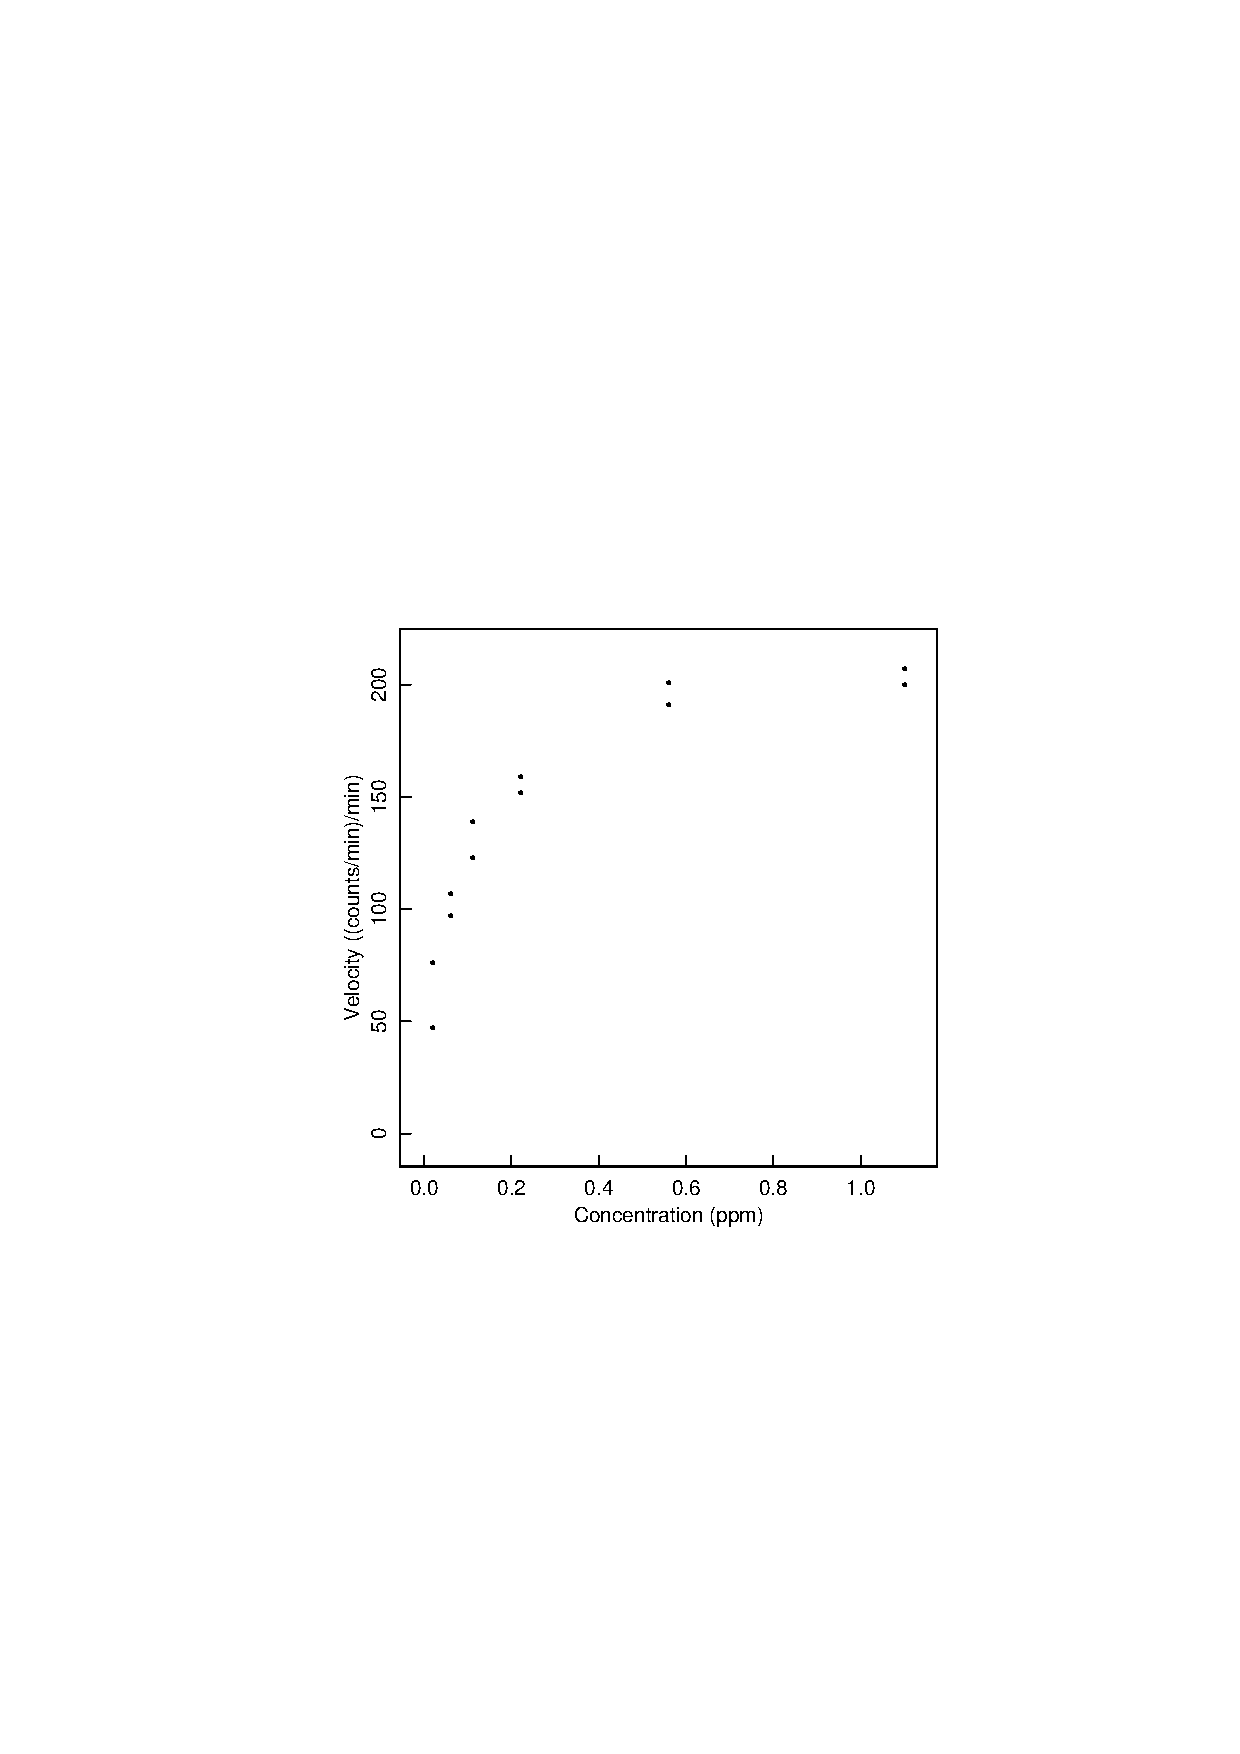
\includegraphics{2MICdata}%height=3in,width=!]{2MICdata}
  \caption{Plot of reaction velocity versus substrate concentration
    for the Puromycin data.}
  \label{fig:MICdata}
\end{figure}

Differentiating $f$ with respect to $\theta_1$ and $\theta_2$ gives
  \begin{eqnarray}\label{eqn:2.4}
    \frac{\partial f}{\partial\theta_1}&=&\frac{x}{\theta_2 + x}\\
    \frac{\partial f}{\partial \theta_2}&=&\frac{-\theta_1 x}{(\theta_2+ x )^2}\nonumber
  \end{eqnarray}
and since both these derivatives involve at least one of the
parameters, the model is recognized as nonlinear.
\end{example}

\subsection{Transformably Linear Models}
\index{nonlinear!model - transformably linear}
\index{transformably linear!model}

The Michaelis--Menten model (\ref{eqn:2.3}) can be transformed to a
linear model by expressing the reciprocal of the velocity as a
function of the reciprocal substrate concentration,
  \begin{eqnarray}\label{eqn:transmm}
    \frac{1}{f}&=&\frac{1}{\theta_1}+\frac{\theta_2}{\theta_1}\frac{1}{x}\\
    &=&\beta_1 + \beta_2 u\nonumber
  \end{eqnarray}

We call such models {\it transformably linear}.  Some authors use the
term ``intrinsically linear'',\index{nonlinear!"model-intrinsically
linear"}\index{"intrinsically linear"!model} but we reserve the term
``intrinsic'' for a special geometric property of nonlinear models, as
discussed in Chapter 7.  As will be seen in Chapter 3, transformably
linear models have some advantages in nonlinear regression because it
is easy to get starting values for some of the parameters.

It is important to understand, however, that a transformation of
the data involves a transformation of the disturbance
term too, which affects the assumptions on it.
Thus, if we
assume the model function (\ref{eqn:2.1}) with an additive, spherical
normal disturbance term is an appropriate representation of the
experimental situation, then these same assumptions will not be
appropriate for the transformed data.
Hence we should use
nonlinear regression on the original data, or else weighted least
squares on the transformed data.
Sometimes, of course, transforming a data set to induce constant variance
also produces a linear expectation function
in which case linear regression can be used on the transformed data.
\label{mic:2}
\begin{example}

Because there are replications in the Puromycin data set, it is
easy to see from
Figure \ref{fig:MICdata}
that the variance of the original data is constant,
and hence that nonlinear regression should be used to estimate
the parameters.
However, the reciprocal data, plotted in
Figure \ref{fig:MICinv}$a$,
  \begin{figure}
    \centerline{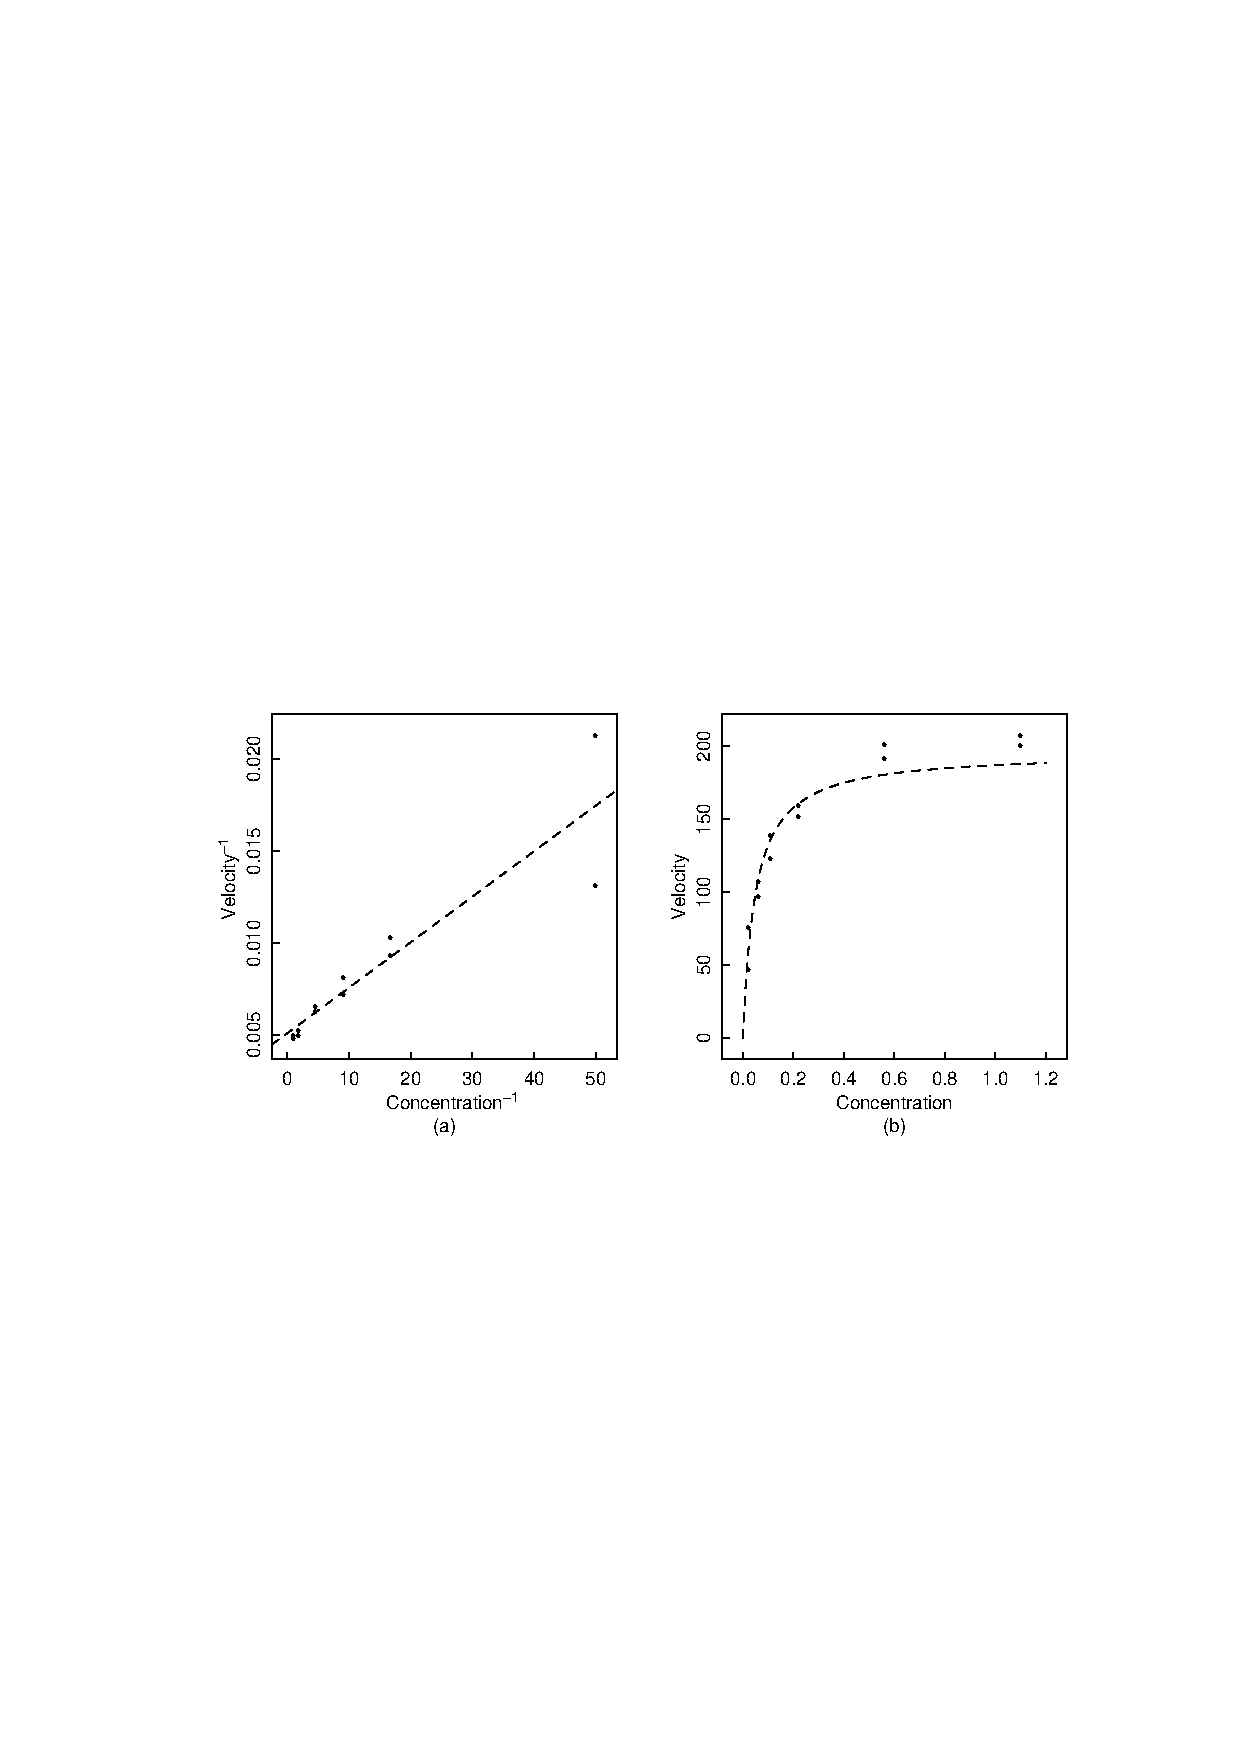
\includegraphics{2MICinv}}%,height=2.25in}}
    \caption[Puromycin Data on Inverse Scale]{\label{fig:MICinv}
    Plot of inverse velocity versus inverse substrate concentration for
    the Puromycin experiment with the linear regression line (dashed)
    in part $a$, and the corresponding fitted curve (dashed) in the original
    scale in part $b$.}
  \end{figure}
while showing a simple straight line relationship,
also show decidely nonconstant variance.
\index{variance!nonconstant}

If we use linear regression to fit the model (\ref{eqn:transmm}) to
these data, we obtain the estimates
  \begin{displaymath}
    \hat{\bbeta}=( 0.005107 ,  0.0002472 ) \trans
  \end{displaymath}
corresponding to
  \begin{displaymath}
    \hat{ \btheta}=( 195.8 ,  0.04841 ) \trans
  \end{displaymath}
The fitted curve is overlaid with the data in the original scale
in Figure \ref{fig:MICinv}$b$, where we see that the predicted
asymptote is too small.
Because the variance of the replicates has been distorted by
the transformation, the cases with low concentration (high
reciprocal concentration) dominate the determination of the
parameters and the curve does not fit the data well at high
concentrations.
\end{example}

This example demonstrates two important features.
First, it
emphasizes the value of replications, because without
\index{replication}
replications it may not be possible to detect either the constant
variance in the original data or the nonconstant variance in the
transformed data; and second, it shows that while transforming
can produce simple linear behavior, it also
affects the disturbances.
\subsection{Conditionally Linear Parameters}
\index{parameter!conditionally linear}

The Michaelis--Menten model is also an example of a model in which
there is a conditionally linear parameter, $\theta_1$.
It is {\it conditionally linear} because the
derivative of the expectation function with respect to
$\theta_1$ does not involve $\theta_1$.
We can therefore estimate $\theta_1$, conditional on $\theta_2$, by a
linear regression of velocity $x/(\theta_2+x)$.
Models with conditionally linear parameters enjoy some advantageous
properties, which can be exploited in nonlinear regression.

\subsection{The Geometry of the Expectation Surface}
\index{geometry}
\index{geometry!of the expectation surface}
\index{expectation surface!geometry}

The assumption of a spherical normal distribution for the disturbance
term $\bZ$ leads us to consider the Euclidean geometry of the
$N$-dimensional response space, because again we will be interested in
the least squares estimates $\hat{ \btheta}$ of the parameters.
The $N$-vectors $\boeta ( \btheta )$ define a $P$-dimensional surface
called the \emph{expectation surface} in the response space, and the
least
\index{response!space}
squares estimates correspond to the point on the expectation
surface\index{expectation surface},
  \begin{displaymath}
    \hat{\boeta}=\boeta(\hat{\btheta})
  \end{displaymath}
which is closest to $\by$.
That is, $\hat{\btheta}$ minimizes the residual sum of squares
  \begin{displaymath}
    S( \btheta ) = \norm \by - \boeta ( \btheta ) \norm^2
  \end{displaymath}
\label{rum:2}
\begin{example}

To illustrate the geometry of nonlinear models,
\index{geometry!of nonlinear models}
consider the two cases $t = 4$ and $t = 41$ for the Rumford data.
Under the assumption that Newton's law of cooling holds for these
data, the expected responses are
\begin{displaymath}
  \boeta ( \theta ) =
  \begin{bmatrix}
    60 + 70  e^{ - 4 \theta }\\60 + 70 e^{ - 41 \theta }
  \end{bmatrix}\quad
  \theta \ge 0
\end{displaymath}
Substituting values for $\theta$ in these equations and
plotting the points in a 2-dimensional response space
gives the 1-dimensional expectation surface (curve)
shown in Figure \ref{fig:RUM2esurf}.
  \begin{figure}
    \centerline{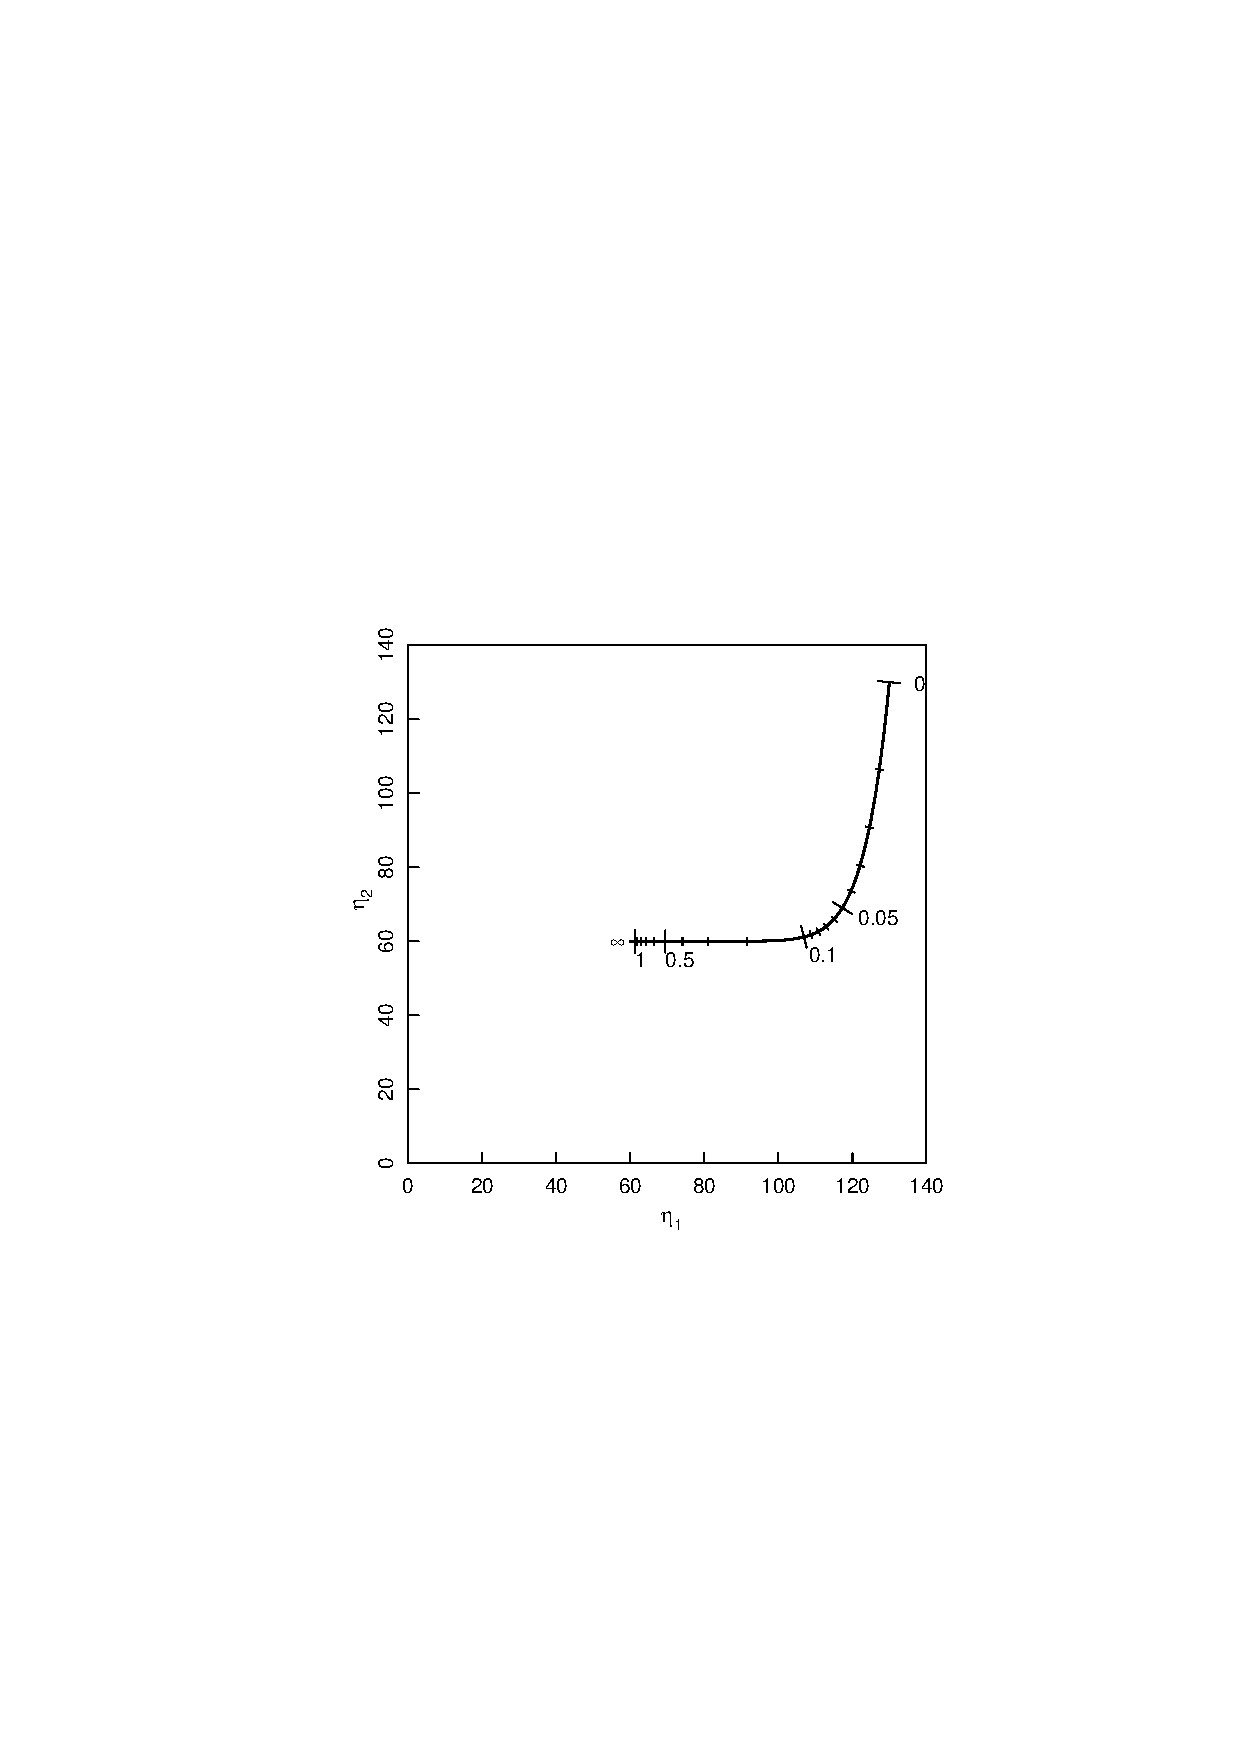
\includegraphics{2RUM2esurf}}%,height=3in}}
    \caption{\label{fig:RUM2esurf}
    Plot of the expectation surface (solid line) in the response space
    for the 2-case Rumford data.  The points corresponding to
    $\theta=0,0.01,0.02,\ldots,0.1,0.2,\ldots,1,\infty$ are marked.
    }
  \end{figure}

Note that the expectation surface is {\it curved} and of {\it finite
extent}, which is in contrast to the linear model in which 
the expectation surface is a plane of infinite extent.
Note, too, that points with equal spacing on the parameter line
($\theta$) map to points with unequal spacing on the expectation
surface.
\end{example}
\label{mic:3}
\begin{example}

As another example, consider the three cases from
Example Puromycin \ref{mic:1}: $x = 1.10$, $x = 0.56$, and
$x = 0.22$.
Under the assumption
that the expectation function (\ref{eqn:2.3}) is the correct one, the
expected responses for these substrate values are
\begin{displaymath}
  \boeta ( \btheta ) =
  \begin{bmatrix}
    \frac{\theta_1(1.10)}{\theta_2+1.10}\\
    \frac{\theta_1(0.56)}{\theta_2+0.56}\\
    \frac{\theta_1(0.22)}{\theta_2+0.22}\\
  \end{bmatrix}
  \quad\theta_1 , \theta_2 \ge 0
  \end{displaymath}
and so we can plot the expectation surface by substituting values
for $\btheta$ in these equations.
A portion of the
2-dimensional expectation surface for these $x$ values is
\index{expectation surface}
shown in
Figure \ref{fig:MICesurf}.
  \begin{figure}
    \centerline{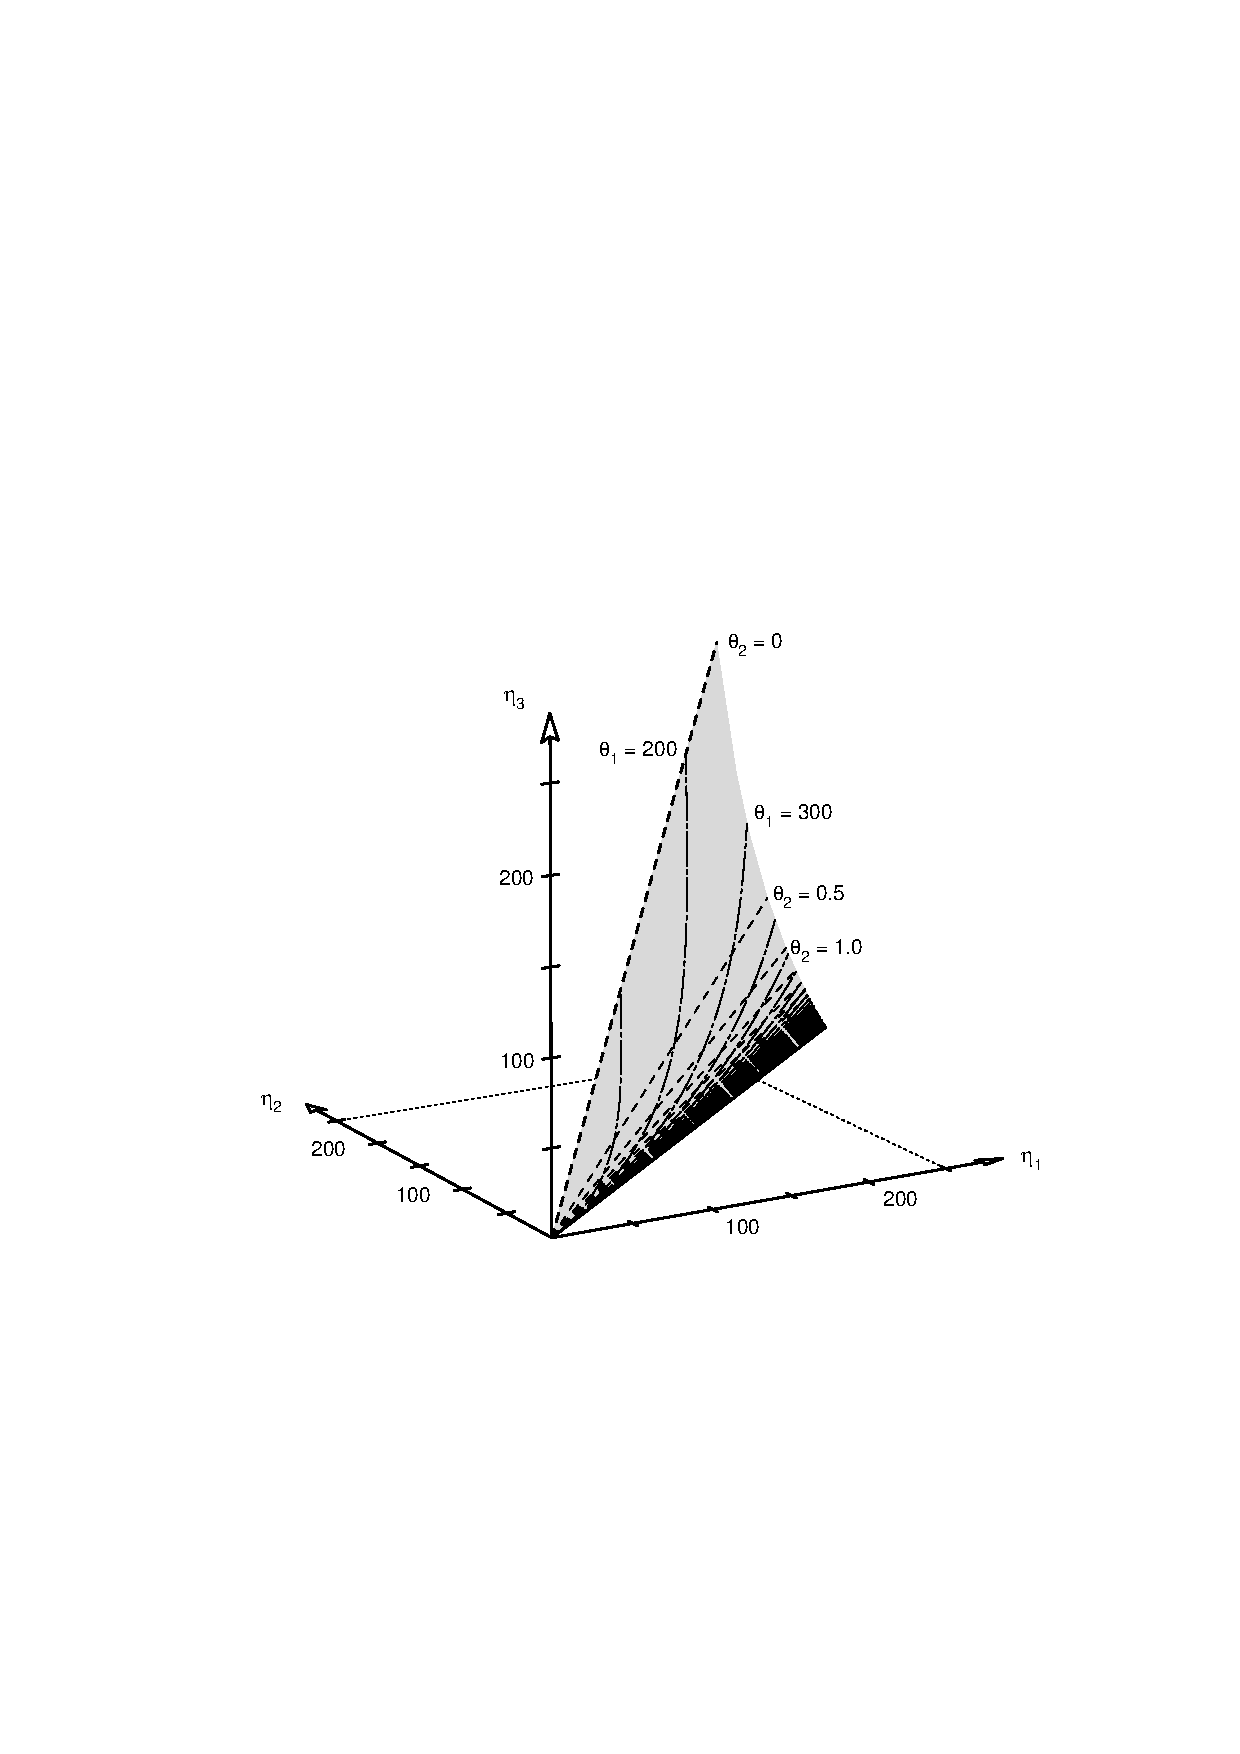
\includegraphics{2MICesurf}}%,height=4.5in}}
    \caption[3-case Puromycin example]{\label{fig:MICesurf}
    Expectation surface for the 3-case Puromycin example.
    We show a portion of the expectation surface (shaded) in the
    expectation space with $\theta_1$ parameter lines (dashed) and
    $\theta_2$ parameter lines (dot--dashed).
    }
  \end{figure}
Again, in contrast to the linear model,
this expectation surface is not an infinite plane, and in
general, straight lines in the parameter plane do not map to
straight lines on the expectation surface.
It is also seen that unit squares in
the parameter plane map to irregularly shaped areas on
\index{parameter!plane}
the expectation surface and that the sizes of these areas
vary.
Thus, the Jacobian determinant is not
\index{Jacobian!determinant}
\index{determinant!Jacobian}
constant, which
can be seen analytically, of course, because the
derivatives (\ref{eqn:2.4}) depend on $\btheta$.

For this model, there are straight lines on the expectation
surface in Figure \ref{fig:MICesurf} corresponding to the $\theta_1$
parameter lines (lines with $\theta_2$ held constant),
\index{parameter!line on expectation surface}
reflecting the fact that $\theta_1$ is conditionally linear.
However, the $\theta_1$ parameter lines are neither parallel
nor equispaced.
The $\theta_2$ lines are not straight, parallel, or equispaced.
\end{example}

As can be seen from these examples, for nonlinear models with
$P$ parameters, it is generally true that:
\begin{enumerate}

  \item the expectation surface, $\boeta ( \btheta )$, is a
        $P$-dimensional {\it curved surface} in the $N$-dimensional
        response space;

  \item parameter {\it lines} in the parameter space map to {\it
        curves} on the curved expectation surface; 

  \item the {\it Jacobian determinant}, which measures how large
        unit areas in $\btheta$ become in $\boeta ( \btheta )$, is
        {\it not constant}.

\end{enumerate}

We explore these interesting and important aspects of the
expectation surface later, but first we discuss how to obtain
the least squares estimates $\hat{ \btheta}$ for the parameters $\btheta$.
Nonlinear least squares estimation from the point of view
of sum of squares contours is given in Section 2.4.

\section{Determining the Least Squares Estimates}

The problem of finding the least squares estimates can be stated
\index{least squares!estimates for nonlinear model}
\index{least squares!geometry}
very simply geometrically---given a data vector
$\by$, an expectation function $f  ( \bx_n ,\btheta )$,
and a set of design vectors $\bx_n$, $n = 1 ,\ldots, N$
\par\vspace{1.0\baselineskip}
%.ln
(1)find the point $ \hat{ \boeta} $ on the expectation surface
which is closest to $\by$, and then
%.ln
(2)determine the parameter vector $\hat{ \btheta}$ which corresponds to the
point $ \hat{ \boeta} $.


For a linear model, step (1) is straightforward because the
expectation surface is a plane of infinite extent, and we
may write down an explicit expression for the point on that
plane which is closest to $\by$,
  \begin{displaymath}
    \hat{ \boeta} = \bQ_1 {\bQ_1 \trans} \by
  \end{displaymath}
For a linear model, step (2) is also straightforward because the
$P$-dimensional parameter plane maps linearly and invertibly to
the expectation plane, so once we know where we are on one plane we
can easily find the corresponding point on the other.  Thus
  \begin{displaymath}
    \hat{ \bbeta} = {\bR_1^{-1}} { \bQ_1 \trans} \hat{ \boeta}
  \end{displaymath}

In the nonlinear case, however, the two steps are very difficult: the
first because the expectation surface is curved and often of finite
extent (or, at least, has edges) so that it is difficult even to find
$\hat{ \boeta}$, and the second because we can map points easily only in one
direction---from the parameter plane to the expectation surface.
That is, even if we know $\hat{ \boeta}$, it is extremely
difficult to determine the parameter plane coordinates $\hat{ \btheta}$
corresponding to that point.
To overcome these difficulties, we use iterative methods to
\index{iteration}
determine the least squares estimates.
\subsection{The Gauss--Newton Method 2 2 1}
\index{Gauss-Newton!method}

An approach suggested by Gauss is to use a linear approximation
to the expectation function to iteratively improve
an initial guess $\btheta^0$
for $\btheta$ and keep improving the
estimates until there is no change.
That is, we expand the expectation function
\index{expectation function!linear approximation to}
\index{linear approximation!to expectation function}
$f  ( \bx_n ,\btheta )$ in a first order Taylor
series about $\btheta^0$ as
  \begin{displaymath}
    f(\bx_n,\btheta)\approx f(\bx_n,\btheta^0)+
    \mbox{\rm v}_{n1} ( \theta_1 - \theta_1^0 ) +
    \mbox{\rm v}_{n2} ( \theta_2 - \theta_2^0 ) + \ldots +
    \mbox{\rm v}_{nP} ( \theta_P - \theta_P^0 )
  \end{displaymath}
where
  \begin{displaymath}
    \mbox{\rm v}_{np}=\left. \frac{\partial f  ( \bx_n ,\btheta )}{
    \partial \theta_p} \right|_{ \theta^0} p = 1, 2 ,\ldots, P
  \end{displaymath}
Incorporating all $N$ cases, we write
  \begin{equation}\label{eqn:2.5}
  \boeta ( \btheta ) \approx
  \boeta ( \btheta^0 ) + \bV^0 ( \btheta - \btheta^0 )
  \end{equation}
where $\bV^0$ is the $N \times P$ derivative matrix with elements
\index{derivative matrix}
\index{matrix!derivative}
$\mbox{\rm v}_{np}$.
This is equivalent to approximating the residuals,
$\bz ( \btheta )   = \by - \boeta ( \btheta )$, by
\index{residual}
  \begin{equation}\label{eqn:2.5a}
  \bz ( \btheta )\approx \by - [ \boeta ( \btheta^0 ) + \bV^0 \bdelta ]
  =\bz^0-\bV^0 \bdelta
  \end{equation}
where $\bz^0=\by-\boeta(\btheta^0)$ and $\bdelta=\btheta-\btheta^0$.

We then calculate the \emph{Gauss increment}\index{Gauss increment}
$\bdelta^0$ to minimize the approximate residual sum of squares
$\norm \bz^0 - \bV^0 \bdelta \norm^2$, using
  \begin{eqnarray*}
    \bV^0&=&\bQ \bR = \bQ_1 \bR_1\hfill\mbox{\rm [cf.(1.19)]}\\
    \bw_1&=&\bQ_1 \trans \bz^0\hfill\mbox{\rm [cf.(1.21)]}\\
    \hat{ \boeta}^1&=&\bQ_1 \bw_1\hfill\mbox{\rm [cf.(1.23)]}
  \end{eqnarray*}
and so
  \begin{displaymath}
    \bR_1 \bdelta^0 = \bw_1\hfill\mbox{\rm [cf.(1.24)]}
  \end{displaymath}
The point
  \begin{displaymath}
    \hat{\boeta}^1=\boeta(\btheta^1)=\boeta(\btheta^0+\bdelta^0)
  \end{displaymath}
should now be closer to $\by$ than $\boeta(\btheta^0)$, and so we move
to this better parameter value $\btheta^1=\btheta^0+\bdelta^0$
and perform another iteration by calculating new residuals
$\bz^1 = \by - \boeta ( \btheta^1 )$, a new derivative
matrix $\bV^1$, and a new increment.
This process is repeated until convergence\index{ convergence} is
obtained, that is, until the increment is so small that there is no
useful change in the elements of the parameter vector.

\begin{example}\label{mic:4}

To illustrate these calculations, consider the data from Example
Puromycin \ref{mic:1}, with the starting estimates
$\btheta^0=(205,0.08)\trans$.
The data, along with the fitted values, residuals, and derivatives
evaluated at $\btheta^0$, are shown in Table \ref{tbl:2.1}.
\begin{table}
  \caption{\label{tbl:2.1} Residuals and derivatives for Puromycin
  data at $\theta=(205,0.08)\trans$.}
  \begin{center}
    \begin{tabular}{l c c c c c c}\hline
      \multicolumn{1}{c}{$n$} & \multicolumn{1}{c}{$x_{n}$} &
      \multicolumn{1}{c}{$y_{n}$} & \multicolumn{1}{c}{$\eta_n^0$} &
      {$z_n^0$} & \multicolumn{1}{c}{${\rm v}_{n1}^0$} & {$ v_{n2}^0$}\\
      \hline 1&0.02&76&41.00&35.00&0.2000&--410.00\\
      2&0.02&47&41.00&6.00&0.2000&--410.00\\
      3&0.06&97&87.86&9.14&0.4286&--627.55\\
      4&0.06&107&87.86&19.14&0.4286&--627.55\\
      5&0.11&123&118.68&4.32&0.5789&--624.65\\
      6&0.11&139&118.68&20.32&0.5789&--624.65\\
      7&0.22&159&150.33&8.67&0.7333&--501.11\\
      8&0.22&152&150.33&1.67&0.7333&--501.11\\
      9&0.56&191&179.38&11.62&0.8750&--280.27\\
      10&0.56&201&179.38&21.62&0.8750&--280.27\\
      11&1.10&207&191.10&15.90&0.9322&--161.95\\
      12&1.10&200&191.10&8.90&0.9322&--161.95\\ \hline
    \end{tabular}
  \end{center}
\end{table}

Collecting these derivatives into the derivative matrix $\bV^0$, we then
perform a \emph{QR} decomposition, from which we generate
$\bw_1=\bQ_1 \trans \bz^0$
and then solve for $\bdelta^0$ using
$\bR_1 \bdelta^0=\bw_1$.
In this case,
$\bdelta^0=(8.03,-0.017)\trans$
and the sum of squares at
$\btheta^1=\btheta^0 +\bdelta^0$
is $S( \btheta^1 )=1206$, which is much
smaller than $S( \btheta^0 ) = 3155$.  We therefore move to
$\btheta^1 = (213.03,  0.063) \trans$ and perform another
iteration.
\end{example}
\label{bod:BODdata}
\begin{example}

As a second example, we consider data on biochemical oxygen demand
(BOD) from \citeasnoun{mars:1967}, reproduced in
%\glossary{ Marske, D.}
Appendix~\ref{atbl:bod}.  The data are plotted in
Figure \ref{fig:BODdata}.
\begin{figure}
  \centerline{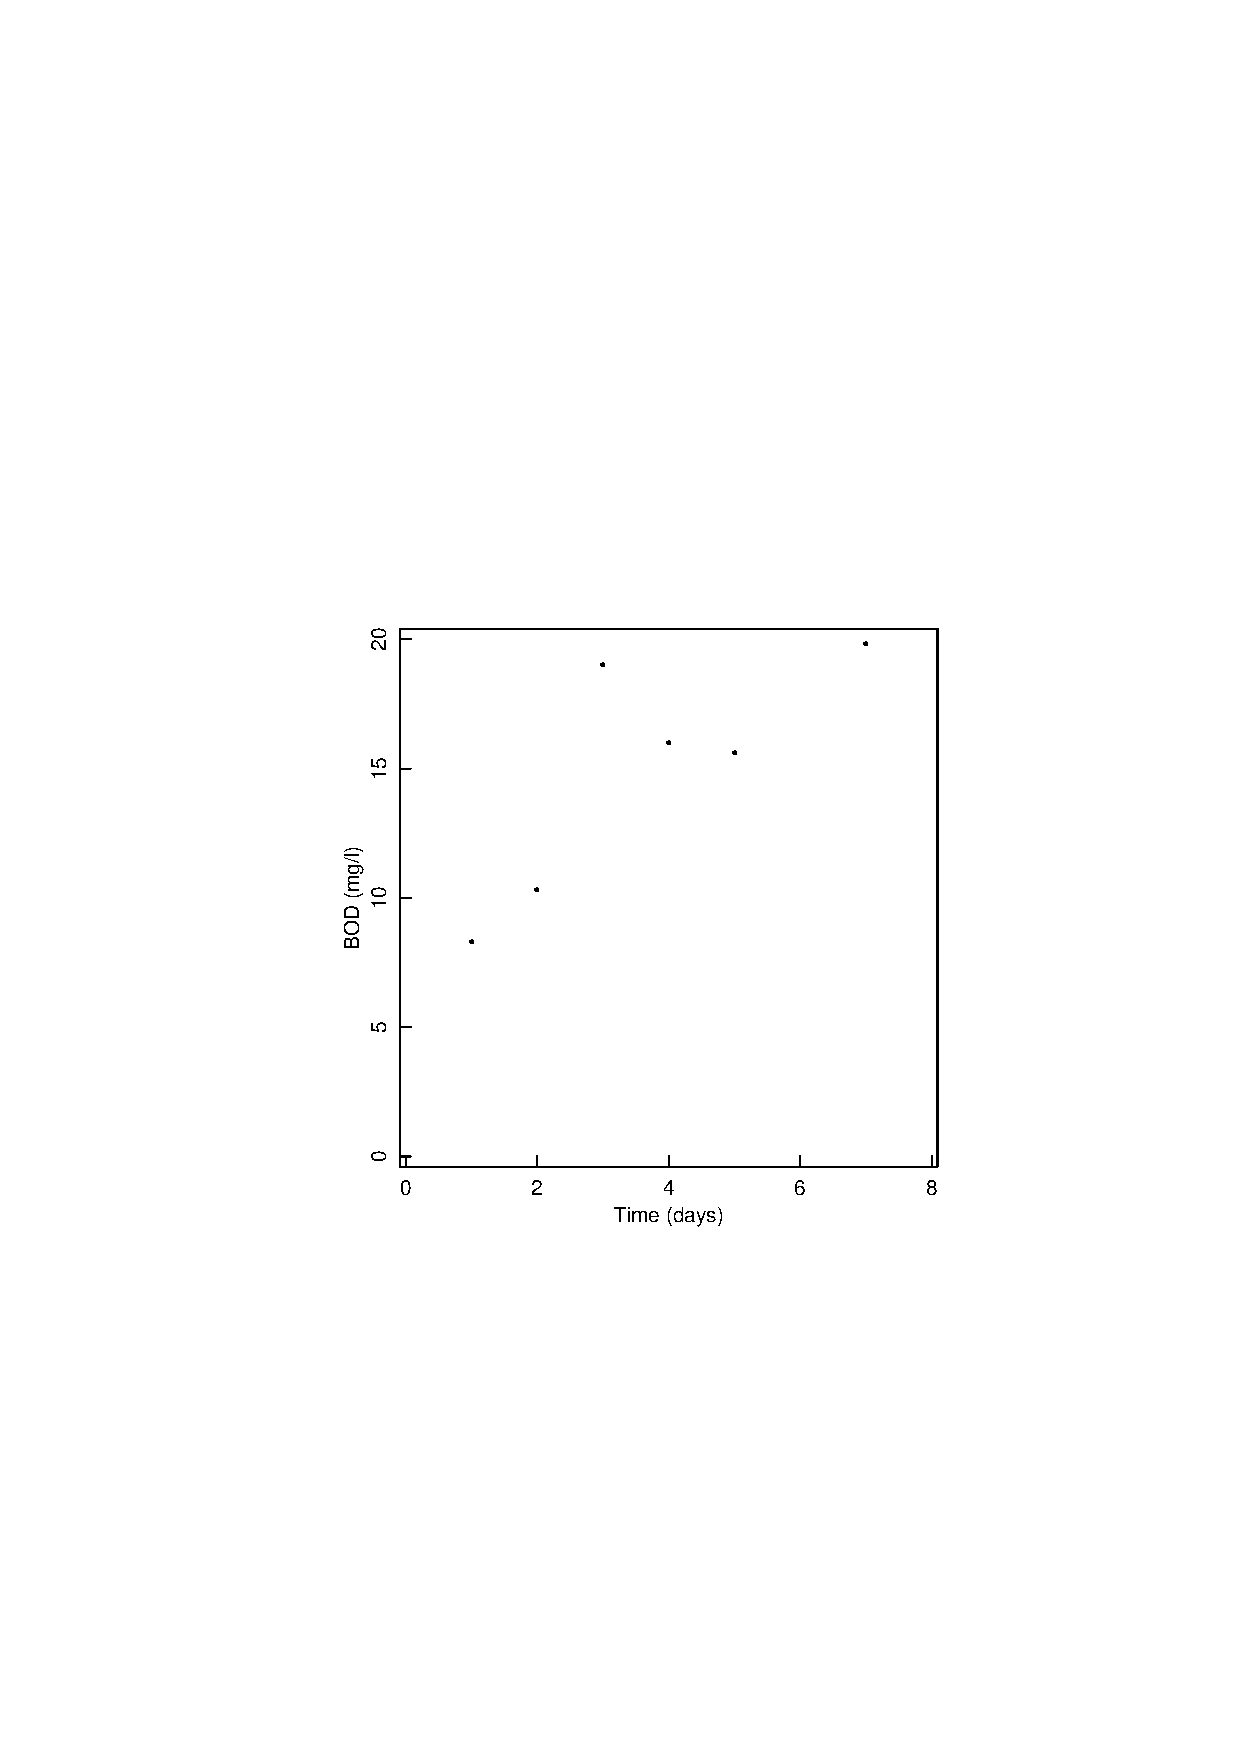
\includegraphics{2BODdata}}%,height=3in}}
  \caption{\label{fig:BODdata}
  Plot of BOD versus time}
\end{figure}
For these data, the model
\begin{equation}\label{eqn:2.6a}
  f(x,\btheta)=\theta_1(1-e^{\theta_2 x})
\end{equation}
is considered appropriate.

Using the starting estimates $\btheta^0=(20,0.24)\trans$,
for which $S ( \btheta^0 )=128.2$, produces an increment to
$\btheta^1 = ( 13.61 ,  0.52 ) \trans$ with $S ( \btheta^1 )
= 145.2$.  In this case, the sum of squares has increased and so
we must modify the increment as discussed below.
\end{example}

\subsection*{Step Factor}
\index{step factor}

As seen in the last example, the Gauss--Newton increment can produce
an \emph{increase}
in the sum of squares when the requested increment
extends beyond the region where the linear approximation
is valid.  Even in these circumstances, however, the linear
approximation will be a close approximation to the actual surface for
a sufficiently small region around $\boeta ( \btheta^0 )$.
Thus a small step in the direction $\bdelta^0$ should produce
a decrease in the
sum of squares.
We therefore introduce a \emph{step factor}
$\lambda$,
and calculate
  \begin{displaymath}
    \btheta^1 = \btheta^0 + \lambda \bdelta^0
  \end{displaymath}
where $\lambda$ is chosen to ensure that
  \begin{equation}\label{eqn:stepfactor}
  S ( \btheta^1 ) < S ( \btheta^0 )
  \end{equation}
A common method of selecting $\lambda$ is to start with $\lambda=1$
and halve it until (\ref{eqn:stepfactor}) is satisfied.  This
modification to the Gauss--Newton algorithm was suggested in
\citeasnoun{box:1960}%\glossary{ Box, G.E.P.} and
\citeasnoun{hart:1961}%\glossary{ Hartley, H.O.}. 

\begin{example}\label{bod:stephalf}
For the data and starting estimates in Example BOD \ref{bod:BODdata},
the value $\lambda = 0.5$ gave a reduced sum of squares, 94.2, at
$\btheta=(16.80,0.38)\trans$. 
\end{example}

Pseudocode for the Gauss--Newton algorithm for nonlinear least
squares is given in Appendix 3, Section A3.1, together with
implementations in GAUSS, S, and SAS/IML.

\subsection{The Geometry of Nonlinear Least Squares}
\index{geometry!of nonlinear least squares}
\index{least squares!geometry of nonlinear}

Geometrically a Gauss--Newton iteration consists of:
  \begin{enumerate}
    \item approximating $\boeta ( \btheta )$ by a Taylor series
          expansion at $\boeta^0 = \boeta ( \btheta^0 )$,
    \item generating the residual vector $\bz^0 = \by - \boeta^0$,
    \item projecting the residual $\bz^0$ onto the tangent plane
          \index{tangent plane}
          to give $\hat{ \boeta}^1$,
    \item mapping $\hat{ \boeta}^1$ through the linear coordinate
          system to produce the increment $\bdelta^0$, and finally
    \item moving to $\boeta ( \btheta^0 + \lambda  \bdelta^0 )$.
  \end{enumerate}

The first step actually involves two distinct approximations:
  \begin{enumerate}
    \item the \emph{planar} assumption, in which we approximate the
          expectation surface
          \index{assumptions!planar}
          \index{planar assumption}
          $\boeta ( \btheta )$ near $\boeta ( \btheta^0 )$ by its
          tangent plane at $\boeta ( \btheta^0 )$, and
    \item the \emph{uniform coordinate} assumption, in which we
          \index{assumptions!uniform coordinate}
          \index{uniform coordinate!assumption}
          impose a linear coordinate system $\bV(\btheta-\btheta^0)$
          on the approximating tangent plane.
  \end{enumerate}

We give geometrical interpretations of these steps and
assumptions in the following examples.

\begin{example}\label{rum:3}
For the 2-case Rumford data set of Example Rumford \ref{rum:2},
we plot $\by$ and a portion of the expectation surface
in Figure \ref{fig:RUM2inc}.
  \begin{figure}
    \centerline{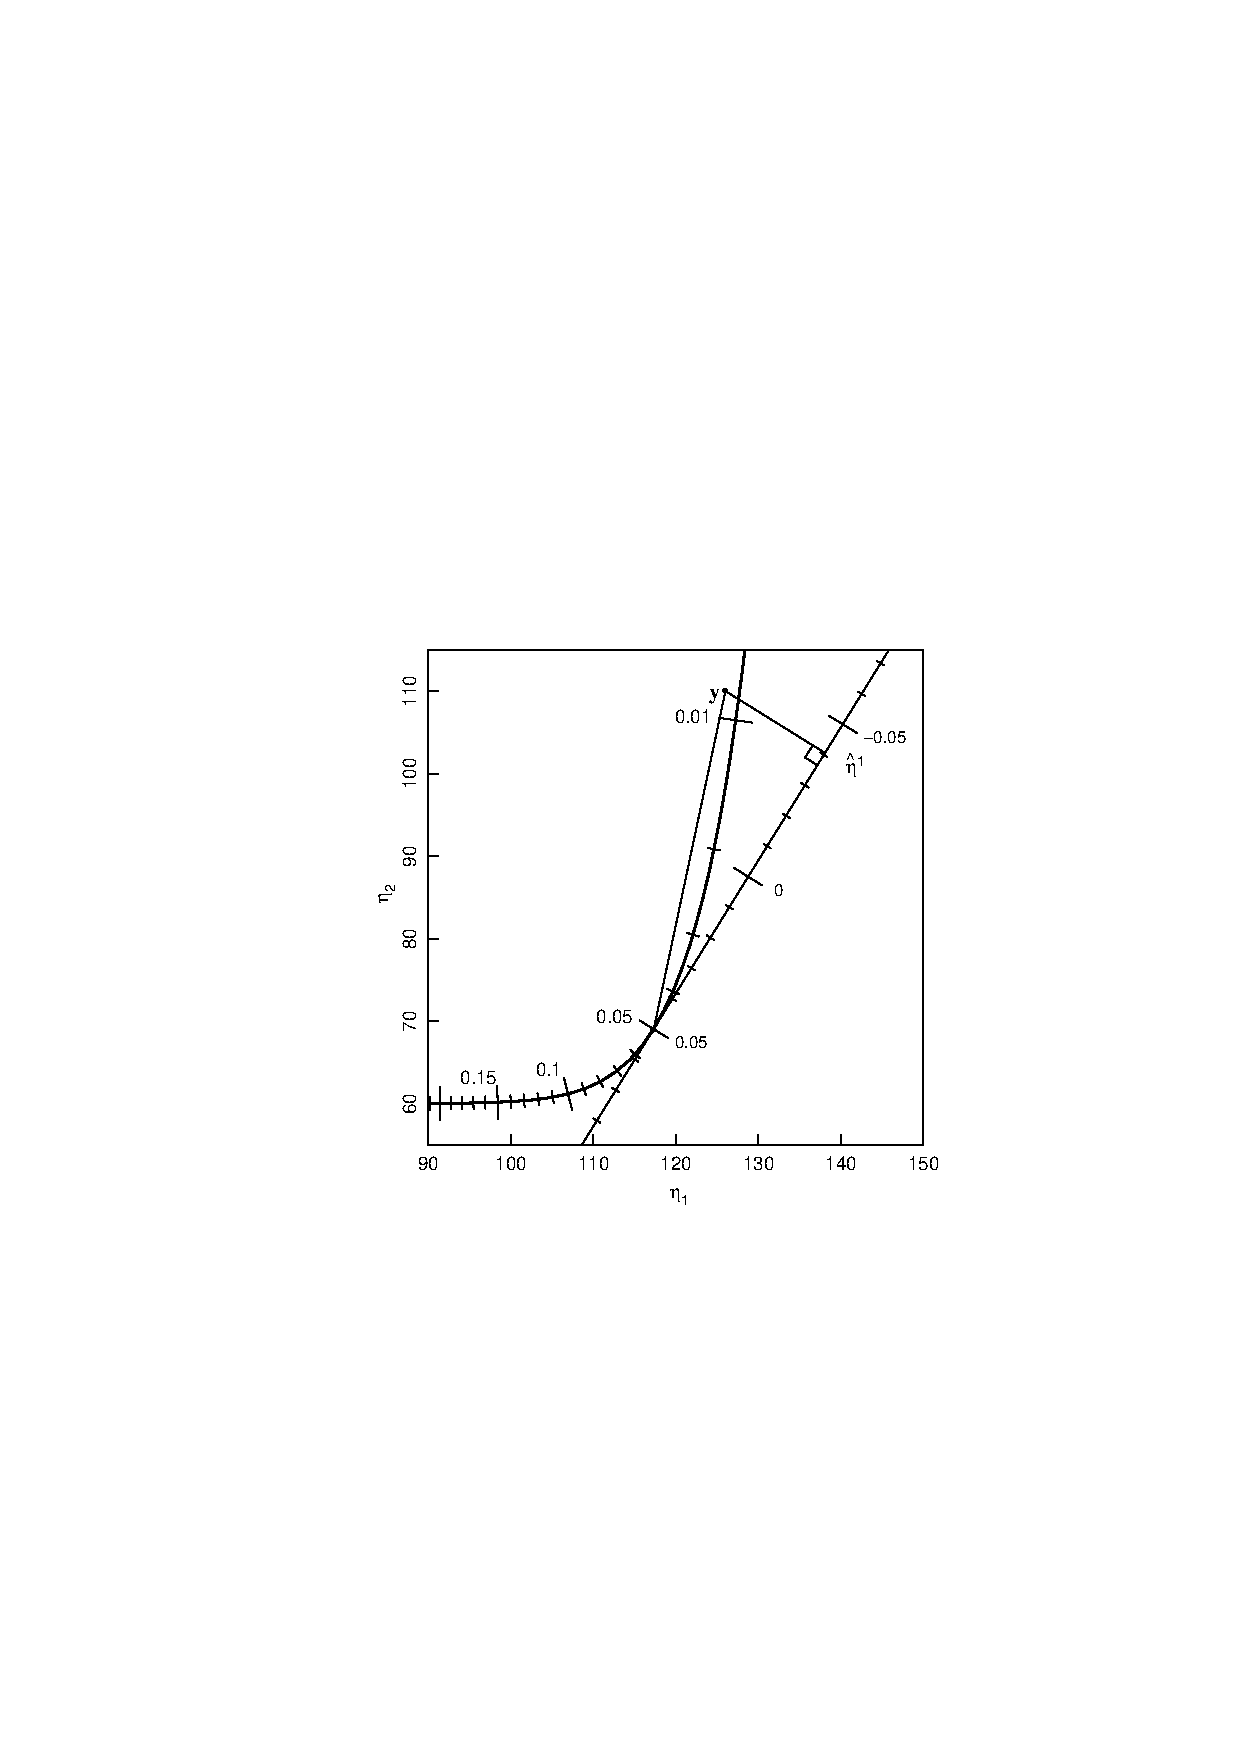
\includegraphics{2RUM2inc}}%,height=3in}}
    \caption[Gauss-Newton increment for the Rumford data]{
    \label{fig:RUM2inc}
    A geometric interpretation of calculation of the Gauss--Newton
    increment using the 2-case Rumford data.
    A portion of the expectation surface (heavy solid line) is shown in
    the response space together with the observed response $\by$.
    Also shown is the projection $\hat{ \boeta}^1$ of
    $\by-\boeta ( 0.05 )$ onto the tangent plane at $\boeta ( 0.05 )$
    (solid line).
    The tick marks indicate true positions on the expectation surface and
    linear approximation positions on the tangent plane.
    }
  \end{figure}
The expectation surface is a curved line, and the points
corresponding to $\theta = 0.01,0.02 ,\ldots, 0.2$ are unevenly
spaced.

For the initial estimate $\theta^0 = 0.05$, a
Gauss--Newton iteration involves the linear approximation
\begin{displaymath}
  \boeta ( \theta ) \approx \boeta^0 + \bv  \delta
\end{displaymath}
where $\delta = ( \theta - 0.05 )$, $\boeta^0$ is the expectation
vector at $\theta = 0.05$,
\begin{displaymath}
  \begin{bmatrix}60 + 70 e^{ -4 \theta }\\60 + 70 e^{ -41 \theta }\end{bmatrix}
  \begin{bmatrix} 117.31 \\ 69.01 \end{bmatrix}
\end{displaymath}
and $\bv$ is the derivative vector at $\theta = 0.05$,
\begin{displaymath}
  \bv =  \begin{bmatrix}- 70(4) e^{ -4 \theta }\\-70(41) e^{ -41 \theta }\end{bmatrix}
  = \begin{bmatrix}-229.25 \\ -369.47 \end{bmatrix}
\end{displaymath}
The Taylor series approximation, consisting of the tangent plane and
the linear coordinate system, is shown as a solid line in
Figure \ref{fig:RUM2inc}.
This replaces the curved expectation surface with the nonlinear
parameter coordinates by a linear surface with a uniform coordinate
system on it.

Next we use linear least squares to obtain the point
$\hat{ \boeta}^1$ on the tangent line which is closest to $\by$.
We then calculate the \emph{apparent} parameter increment
$\delta^0$ corresponding to $\hat{ \boeta}^1$ and from this
obtain $\theta^1 = \theta^0 + \delta^0$.
For this example,
\begin{displaymath}
  \bz^0 =
  \begin{bmatrix}126 \\ 110 \end{bmatrix}
  - \begin{bmatrix} 117.31 \\ 69.01 \end{bmatrix}
  =  \begin{bmatrix} 8.69 \\ 40.99\end{bmatrix}
\end{displaymath}
so
$\hat{ \boeta}^1 = ( 138.1 ,  102.5 ) \trans$,
$\delta^0 = -0.091$, and
$\theta^1=0.05-0.091=-0.041$.

It is clear that the linear approximation increment is too large,
since $\theta^1 = -0.041$, whereas we can see from the points on
the expectation surface that $\hat{ \theta}$ is near 0.01.
We must therefore use a step factor to reduce the increment before
proceeding.
\end{example}
\par\vspace{-6.0pt}
\label{mic:5}
\begin{example}

For a two parameter example, we consider the data and the
starting values from Example Puromycin \ref{mic:4}.
Since the response space is 12-dimensional, we cannot picture it
directly, but we can represent the salient features in the
3-dimensional space spanned by the tangent plane and the
residual vector.
\begin{figure}
  \centerline{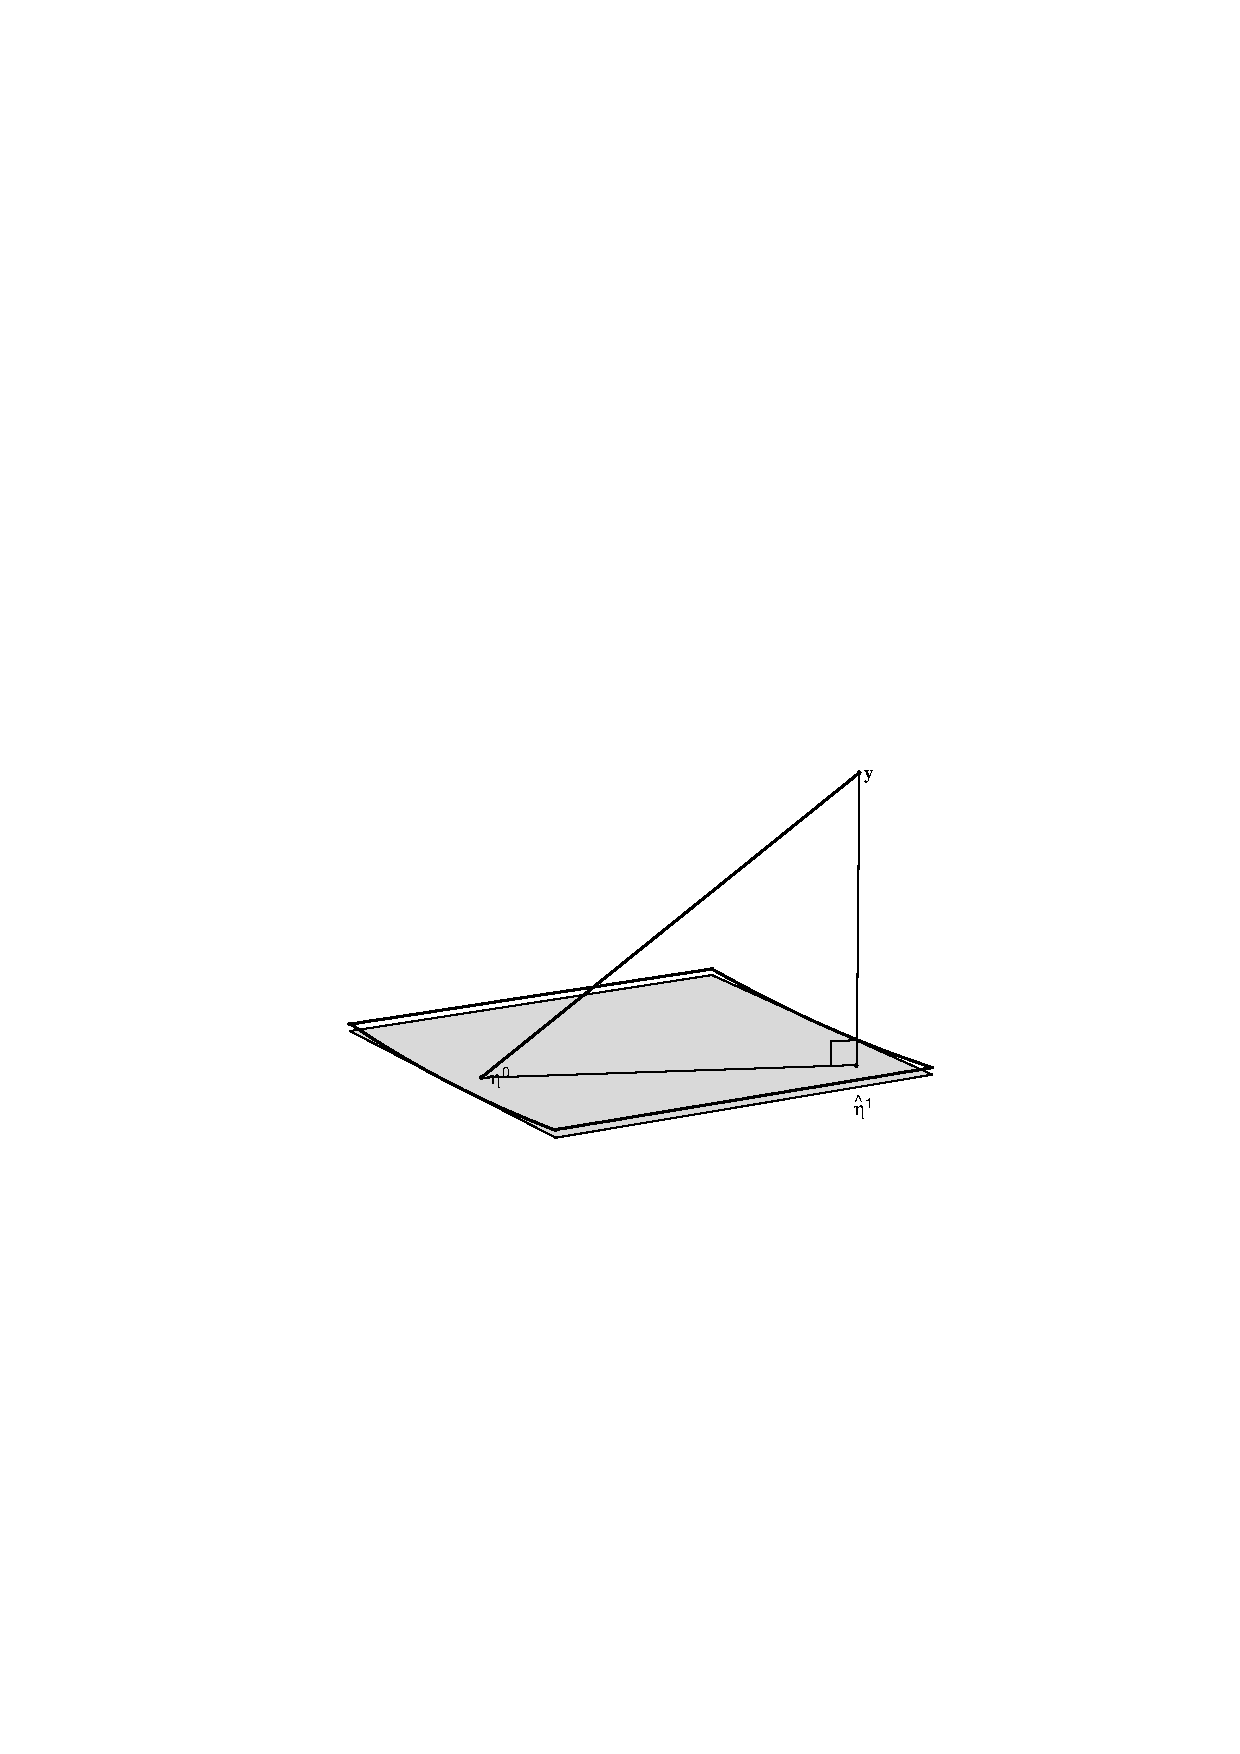
\includegraphics{2MICintrinsic}}%,height=3in}}
  \caption[Gauss-Newton increment for Puromycin data]{
    \label{fig:MICintrinsic}
    A geometric interpretation of calculation of the Gauss--Newton
    increment using the full Puromycin data set.
    We show the projection of a portion of the expectation surface into the
    subspace spanned by the tangent plane at $\boeta^0$
    (shaded) and the residual vector $\by-\boeta^0$.
    The region on the expectation surface is bordered by
    the heavy solid lines.
    Also shown is the projection $\hat{ \boeta}^1$ of the residual
    vector onto the tangent plane.
  }
\end{figure}
We do this in Figure \ref{fig:MICintrinsic}, where we show a portion
of the curved expectation surface, the residual vector, and the
approximating tangent plane.
\index{tangent plane!approximation to expectation surface}
It can be seen that the expectation surface is
only slightly curved, and so is well approximated by the tangent
plane.
\begin{figure}
  \centerline{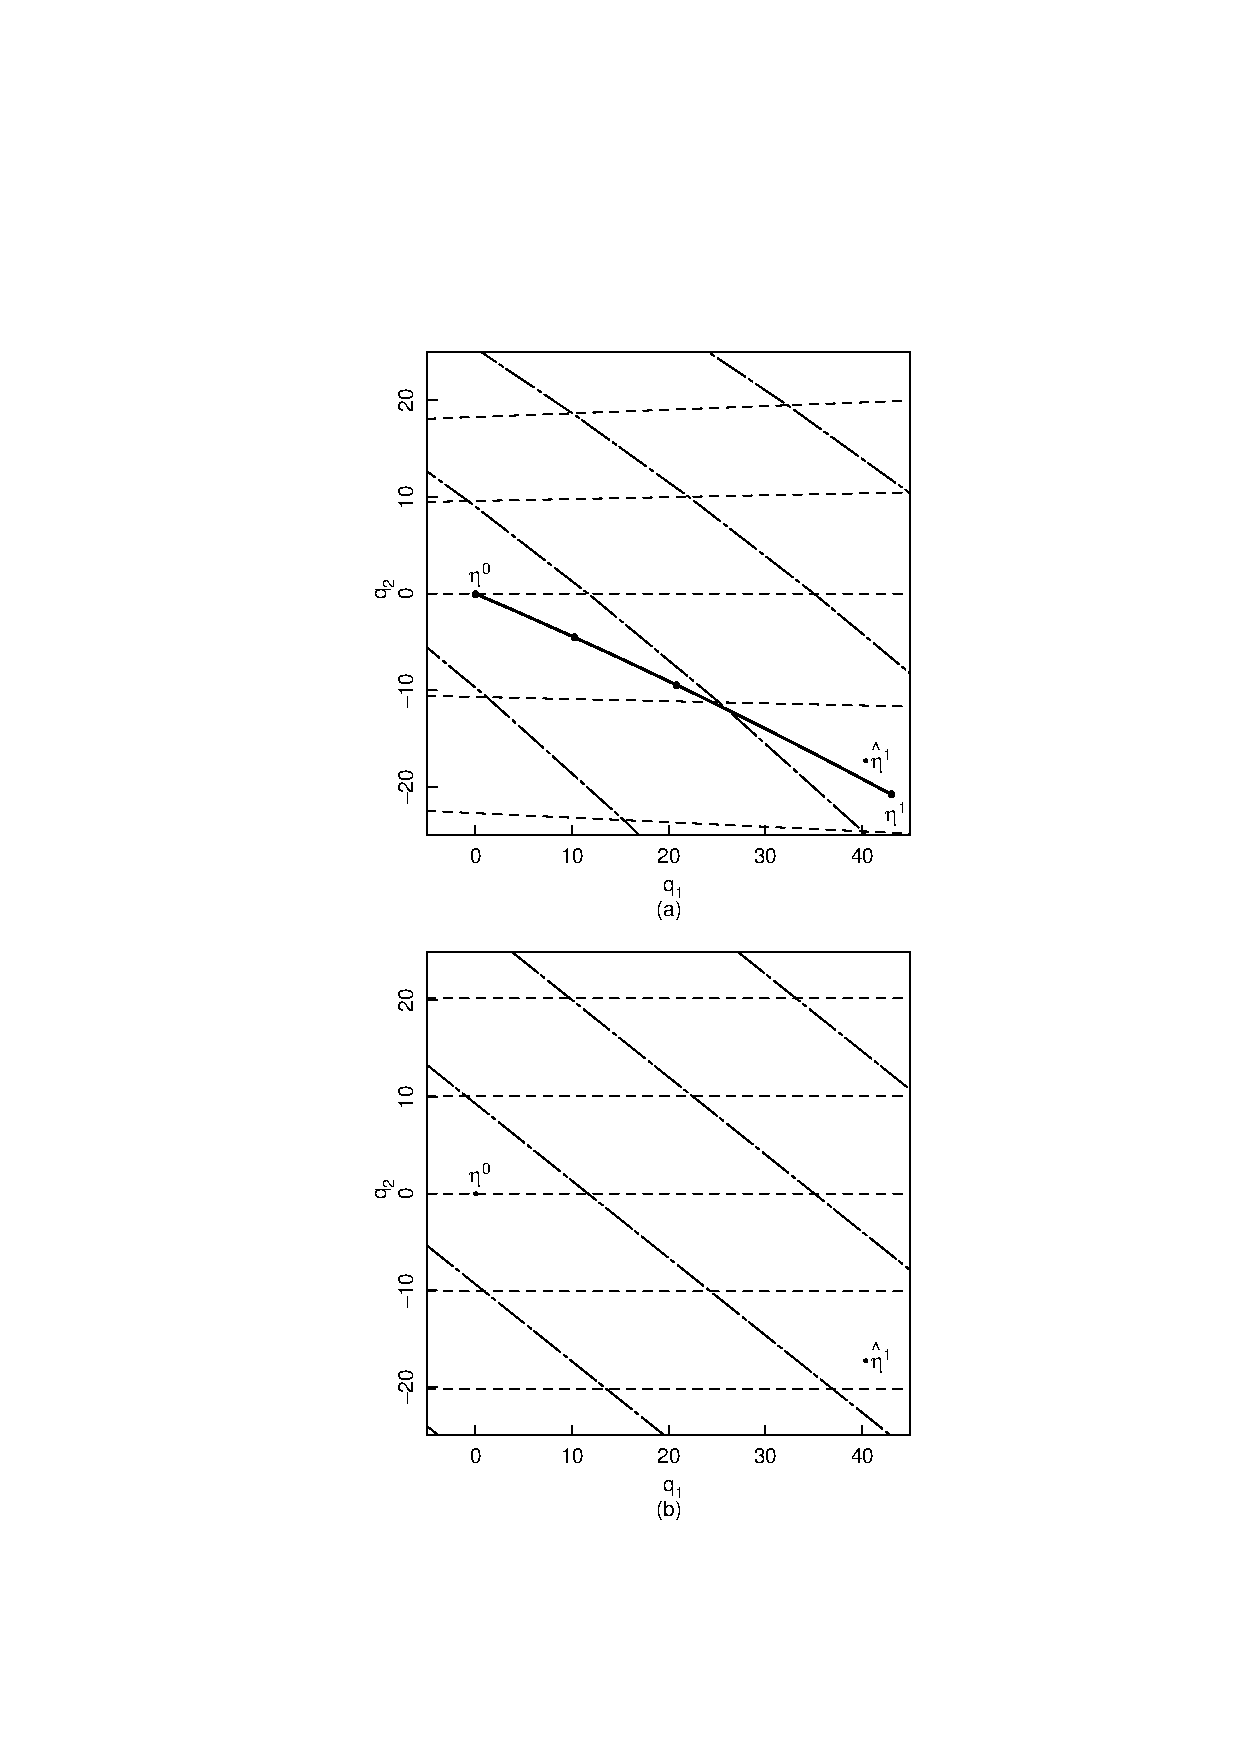
\includegraphics{2MICpeffects}}%,width=\textwidth}}
  \caption[Gauss-Newton increment for Puromycin data]{
    \label{fig:MICpeffects}
    A geometric interpretation of calculation of the Gauss--Newton
    increment using the full Puromycin data set (continued).
    The points $\boeta^0$ and $\hat{ \boeta}^1$ are shown in the
    tangent planes together with the parameter curves in part $a$ and the
    linear approximation parameter lines in part $b$.
    In part $a$ we also show the projection $\boeta^1$ of the point
    $\boeta(\btheta^0+\bdelta^0 )$.
    The curve (heavy solid line) joining $\boeta^0$ to $\boeta^1$ is
    the projection of $\boeta ( \btheta^0+\lambda\bdelta^0 )$ for
    $0\le\lambda\le1$.
    The points corresponding to $\lambda = 0.25$ and $0.5$ are marked.
  }
\end{figure}

In Figure \ref{fig:MICpeffects}$a$ we show the parameter curves for
\index{parameter!curve}
$\theta_1 = 200,210,220,230$ and
$\theta_2 = 0.06,0.07 ,\ldots,0.1$ projected onto the tangent plane,
and in Figure \ref{fig:MICpeffects}$b$ the corresponding linear
approximation lines on the tangent plane.
\index{parameter!linear approximation line to curve}
It can be seen that the linear approximation lines
match the true parameter curves very well.
Also shown on the tangent planes are the points $\boeta^0$
and $\hat{ \boeta}^1$ and in Figure \ref{fig:MICpeffects}$a$ the
projection of the curve
$\boeta ( \btheta^0 + \lambda  \bdelta^0 )$ for
$0 \le \lambda \le 1$.
The points corresponding to $\lambda = 0.25, 0.5$, and
$1$ ($\boeta^1$) are marked.

Because the planar and uniform coordinate assumptions are both
\index{planar assumption}
\index{uniform coordinate!assumption}
valid, the points $\hat{ \boeta}^1$ and $\boeta^1$ are close
together and are much closer to $\by$ than $\boeta^0$.
In this case, a full step ($\lambda = 1$) can be taken resulting
in a decrease in the sum of squares as shown in Example
Puromycin \ref{mic:4}.
\end{example}
\par\vspace{5.0pt}
\label{bod:1}
\begin{example}

As a second two-parameter example, we consider the data and
starting values from Example BOD \ref{bod:BODdata}.
  \begin{figure}
    \centerline{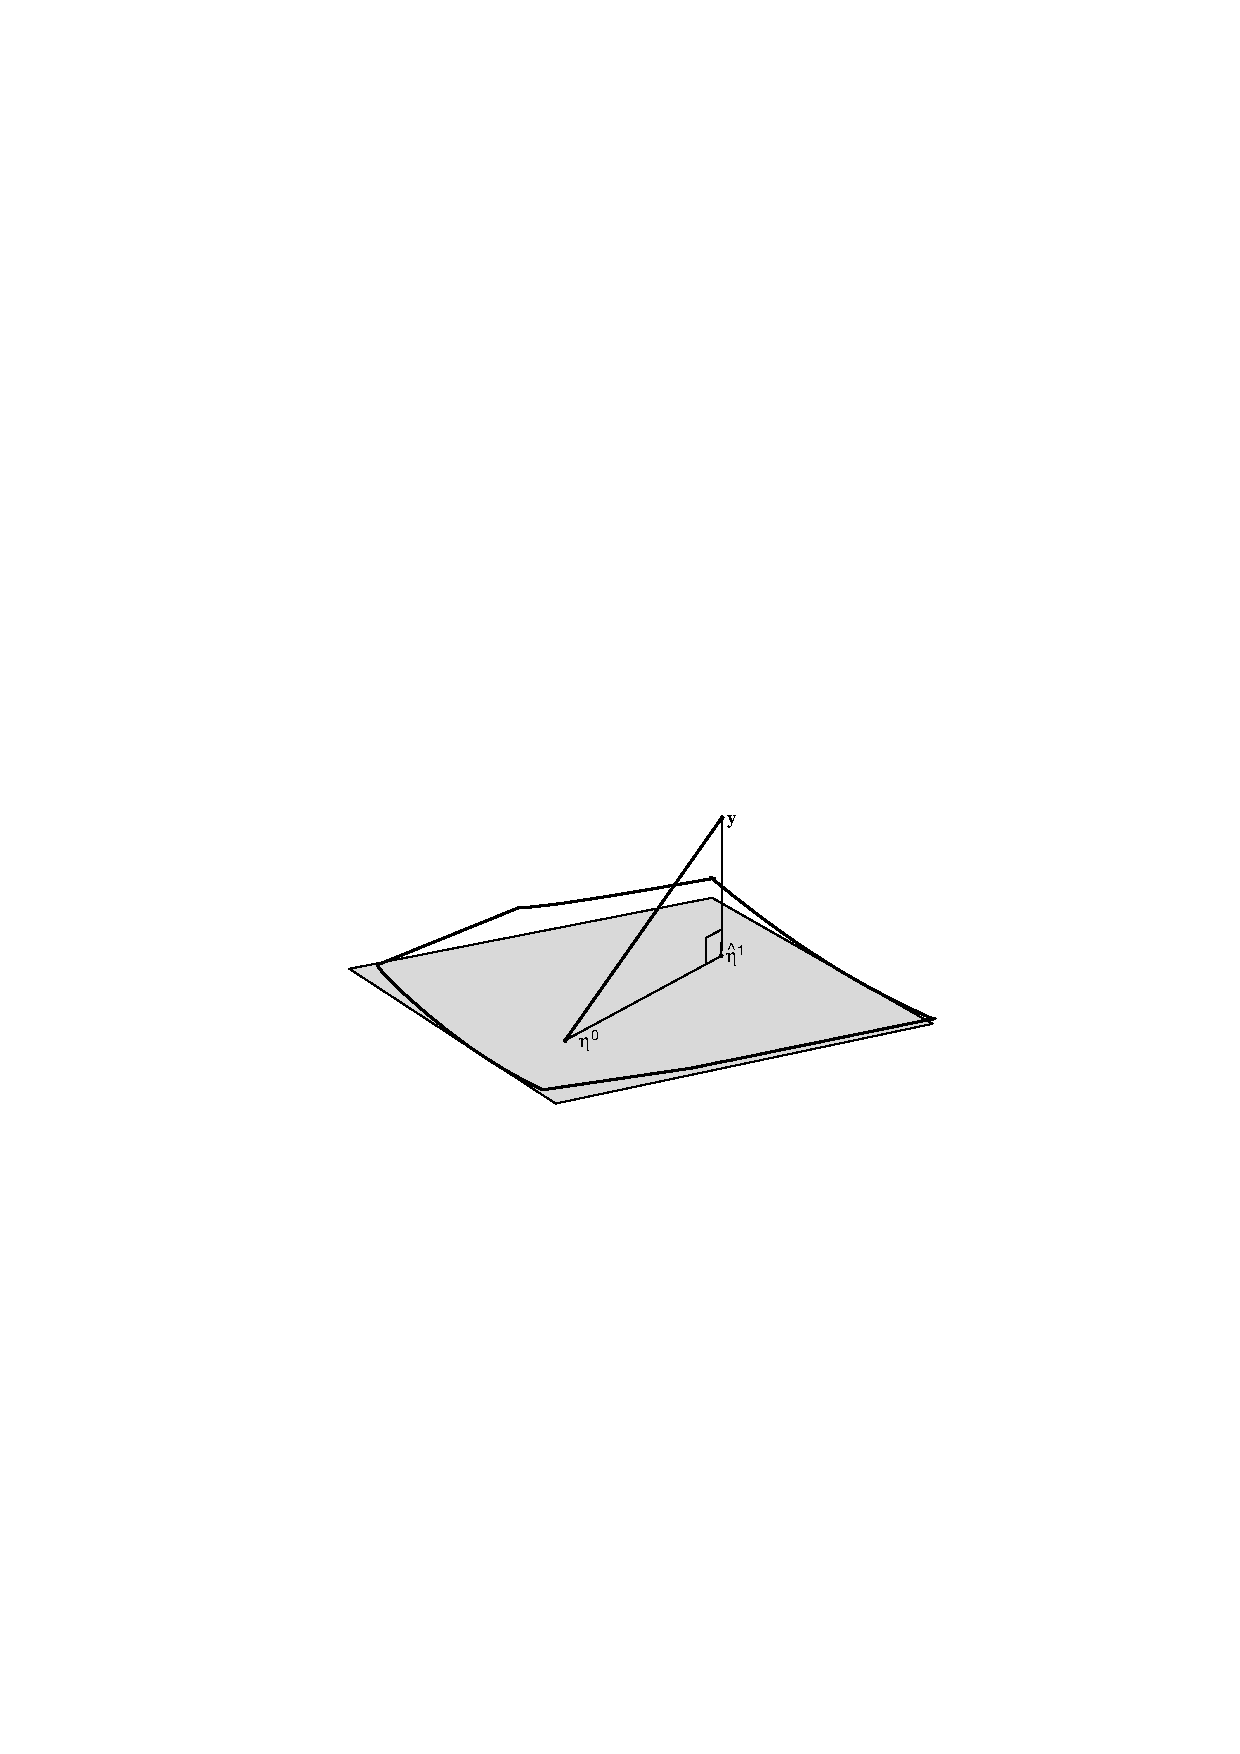
\includegraphics{2BODintrinsic}}%,height=3in}}
    \caption[Gauss-Newton increment for BOD data]{
    \label{fig:BODintrinsic}
    A geometric interpretation of calculation of the Gauss--Newton
    increment using the BOD data set.
    We show the projection of a portion of the expectation surface into the
    subspace spanned by the tangent plane at $\boeta^0$
    (shaded) and the residual vector $\by-\boeta^0$.
    The region on the expectation surface is bordered by
    the heavy solid lines.
    Also shown is the projection $\hat{ \boeta}^1$ of the residual
    vector onto the tangent plane.
    }
  \end{figure}
In Figure \ref{fig:BODintrinsic} we show a
portion of the curved expectation surface,
the residual vector, and the approximating tangent plane
in the space spanned by the tangent plane and the residual vector.
It can be seen that
the expectation surface is moderately curved, but is still apparently
well approximated by the tangent plane.
\index{tangent plane!approximation to expectation surface}
\index{planar assumption}
In this example, the edge of the finite expectation surface is shown as
the angled solid line along the top edge of the surface.
  \begin{figure}
    \centerline{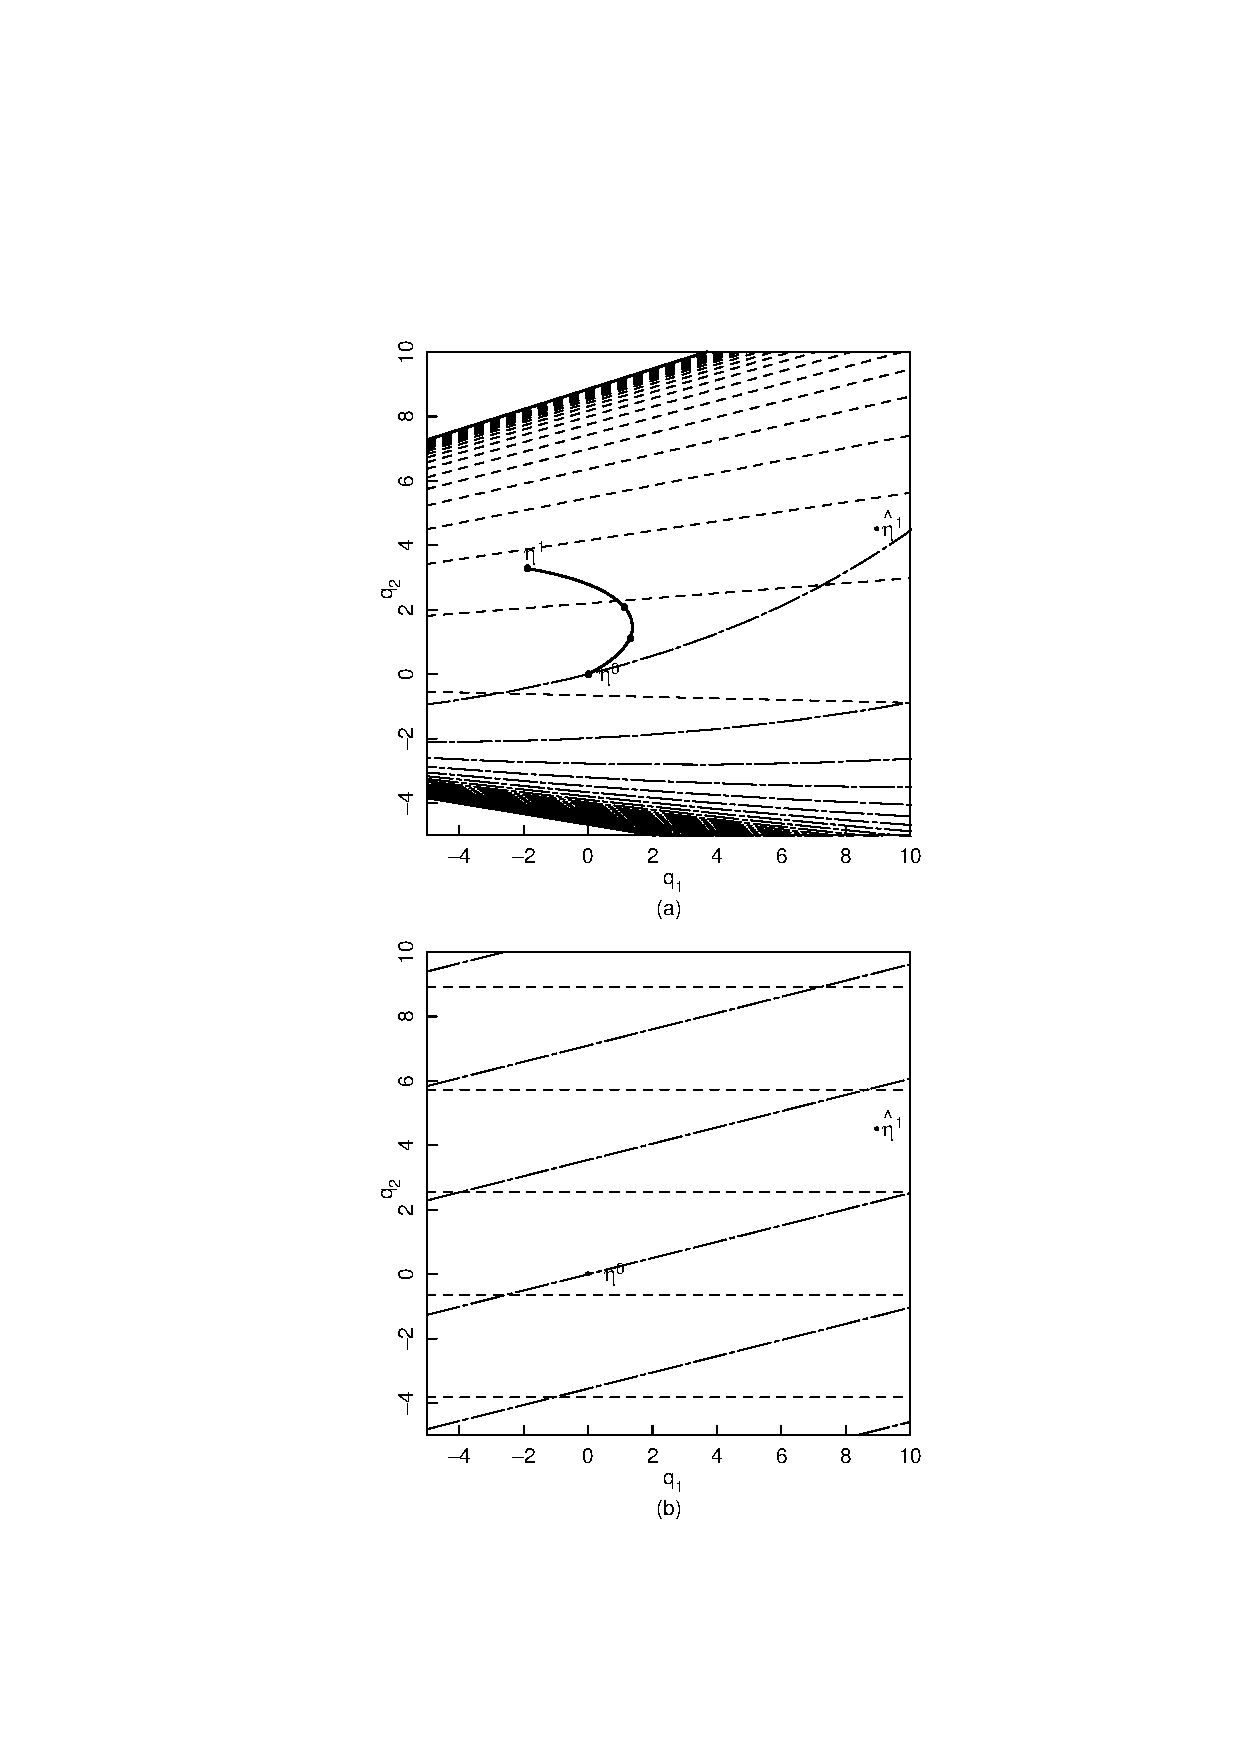
\includegraphics{2BODpeffects}}%,width=\textwidth}}
    \caption[Gauss-Newton increment]{\label{fig:BODpeffects}
    A geometric interpretation of calculation of the Gauss--Newton
    increment using the BOD data set (continued).
    The points $\boeta^0$and $\hat{ \boeta}^1$ are shown in the
    tangent planes together with the parameter curves in part $a$ and
    the linear approximation parameter lines in part $b$.
    In part $a$ we also show the projection $\boeta^1$ of the point
    $\boeta ( \btheta^0+\bdelta^0 )$.
    The curve (heavy solid line) joining $\boeta^0$ to $\boeta^1$ is
    the projection of $\boeta ( \btheta^0+\lambda\bdelta^0 )$ for
    $0\le\lambda\le1$.
    The points corresponding to $\lambda = 0.25$ and $0.5$ are marked.
    }
  \end{figure}

In Figure \ref{fig:BODpeffects}$a$ we show the parameter curves for
$\theta_1 = 20,30,\ldots$ and
$\theta_2 = 0.2,0.4,\ldots$ projected onto the tangent plane.
In Figure \ref{fig:BODpeffects}$b$ we show the corresponding linear
approximation lines on the tangent plane.
\index{parameter!linear approximation line to curve}
In this case, the linear approximation lines
do not match the true parameter curves well at all.
Also shown on the tangent planes are the points $\boeta^0$
and $\hat{ \boeta}^1$, and in Figure \ref{fig:BODpeffects}$a$ the
projection of the curve
$\boeta ( \btheta^0 + \lambda  \bdelta^0 )$ for
$0 \le \lambda \le 1$.
The points corresponding to $\lambda = 0.25, 0.5$, and
$1$ ($\boeta^1$) are marked.

Because the uniform coordinate assumption is not valid this far from
$\btheta^0$,
\index{uniform coordinate!assumption}
the points $\hat{ \boeta}^1$ and $\boeta^1$ are widely
separated, and in fact $\boeta^1$ is farther from
$\hat{ \boeta}^1$ than is $\boeta^0$.
In this case, the reduced step, $\lambda =0.5$, is successful,
as was shown in Example BOD \ref{bod:stephalf}.
\end{example}

To summarize, geometrically we are using local information to
generate a tangent plane with a linear coordinate system dictated
by the derivative vectors, projecting the residual vector onto
that tangent plane, and then mapping the tangent plane
coordinates to the parameter plane using the linear mapping.

\subsection{Convergence}

We have indicated that the Gauss--Newton iterative method is
continued until the values of $\btheta$ on successive
iterations stabilize.
This can be measured by the size of each parameter increment
relative to the previous parameter value, which is the basis for
one of the common criteria used to declare convergence
\index{convergence!criterion}
\cite{bard:1974,drap:smit:1981,jenn:samp:1968,rals:jenn:1978,kenn:gent:1980}.
%(Bard, 1974; Draper and Smith, 1981; Jennrich and Sampson, 1968;
%Kennedy and Gentle, 1980; Ralston and Jennrich, 1978).
%\glossary{ Bard, Y.}
%\glossary{ Draper, N.R.}
%\glossary{ Smith, H.}
%\glossary{ Jennrich, R.I.}
%\glossary{ Sampson, P.F.}
%\glossary{ Kennedy, W.J.Jr.}
%\glossary{ Gentle, J.E.}
%\glossary{ Ralston, M.L.}
Another criterion for convergence used, for example, in
SAS \cite{SAS:1985:stat}, is that the relative
change in the sum of squares on successive iterations be small.
\citeasnoun{Himm:1972} recommends that both these criteria be used,
%\glossary{Himmelblau, D.M.}
since compliance with one does not imply compliance with the other.
However, compliance even with both relative change criteria does
not guarantee convergence, as discussed in \citeasnoun{bate:watt:1981:tech}.
%\glossary{ Bates, D.M.}
%\glossary{ Watts, D.G.}
\citeasnoun{kenn:gent:1980} mention a relative step size criterion
%\glossary{ Kennedy, W.J.Jr.}
%\glossary{ Gentle, J.E.}
as well as relative change in the sum of squares and gradient
size criteria.
\citeasnoun{cham:1977} quotes several other criteria, including the size
%\glossary{ Chambers, J.M.}
of the gradient, the size of the Gauss--Newton step, and the
fact that the residual vector should be orthogonal to the
derivative vectors; but no scale is suggested.

The main criticism of these criteria is that they indicate lack of
progress rather than convergence.
In most cases, of course, lack of progress occurs because a
minimum is encountered: nevertheless, situations can occur where
the parameter increment and sum of squares convergence criteria
indicate lack of progress and yet a minimum has not been reached.

Examination of the geometry of nonlinear least squares provides a
better procedure for determining convergence
(Bates and Watts, 1981b).
%\cite{Bates Watts 1981 techno}
%\glossary{ Bates, D.M.}
%\glossary{ Watts, D.G.}
\index{convergence!geometry}
\index{geometry!of convergence}
We know that a critical point is reached whenever the residual
vector $\by - \boeta ( \btheta )$ is orthogonal to
the expectation surface and therefore to the tangent plane to
the expectation surface at $\boeta ( \btheta )$.
We can thus adopt orthogonality of the residual vector to the
tangent plane as a convergence criterion.
\index{convergence!orthogonality criterion}

In practice, it would be unusual to obtain exact orthogonality in
the presence of numerical roundoff, and we do not want to waste
effort calculating small changes in the parameter vector while
trying to achieve perfect orthogonality.
We therefore need to establish a \emph{tolerance level}
\index{convergence!tolerance level}
which we
can use to declare the residual vector to be ``sufficiently orthogonal.''
One way to do this is to consider the statistical variability in
the least squares estimates.

If we assume that the tangent plane forms a good approximation to
the expectation surface near $\hat{ \btheta}$, so a likelihood
region for $\btheta$ roughly corresponds to a disk on the
tangent plane with a radius proportional to
$\sqrt{S ( \hat{ \btheta} )}$, then we can measure the relative
offset of the current parameter values from the exact least
squares estimates by calculating the ratio of the length of the
component of the residual vector in the tangent plane to
$ \sqrt {S ( \hat{ \btheta} )}$.
When this ratio is small, the numerical uncertainty of the least
squares estimates is negligible compared to the statistical
uncertainty of the parameters.

Unfortunately, this criterion involves the unknown least squares
vector $\hat{ \btheta}$.
We therefore modify the criterion by substituting the current estimate,
$\btheta^i$, for $\hat{ \btheta}$, and
measure the scaled length of the tangent plane component of the residual
vector relative to the scaled length of the orthogonal component of the
residual vector at $\btheta^i$.
This leads to a \emph{relative offset convergence criterion}
\index{convergence!relative offset criterion}
  \begin{equation}\label{eqn:2.7}
  \frac{{\norm \bQ_1 \trans ( \by - \boeta ( \btheta^i ) ) \norm} / \sqrt P
  }{{\norm \bQ_2 \trans ( \by - \boeta ( \btheta^i ) ) \norm} /
  \sqrt{N -P}}
  \end{equation}
where $\bQ_1$ and $\bQ_2$ are the first $P$ and last $N - P$
columns respectively of the matrix $\bQ$ from a \emph{QR} decomposition
of $\bV$.
The criterion is related to the cotangent of the angle
that the residual vector makes with the tangent plane, so that a
small relative offset corresponds to an angle near 90$^\circ$.

To declare convergence, we require the relative offset to be less than
0.001, reasoning that any inferences will not be
affected materially by the fact that the current parameter vector is less
than 0.1\% of the radius of the confidence
region disk from the least squares point.
\label{rum:4}
\begin{example}

We illustrate the convergence criterion and its development with the
2-observation Rumford example.
We wish to test whether the parameter value
$\theta=0.01$ could be considered a point of convergence.
  \begin{figure}
    \centerline{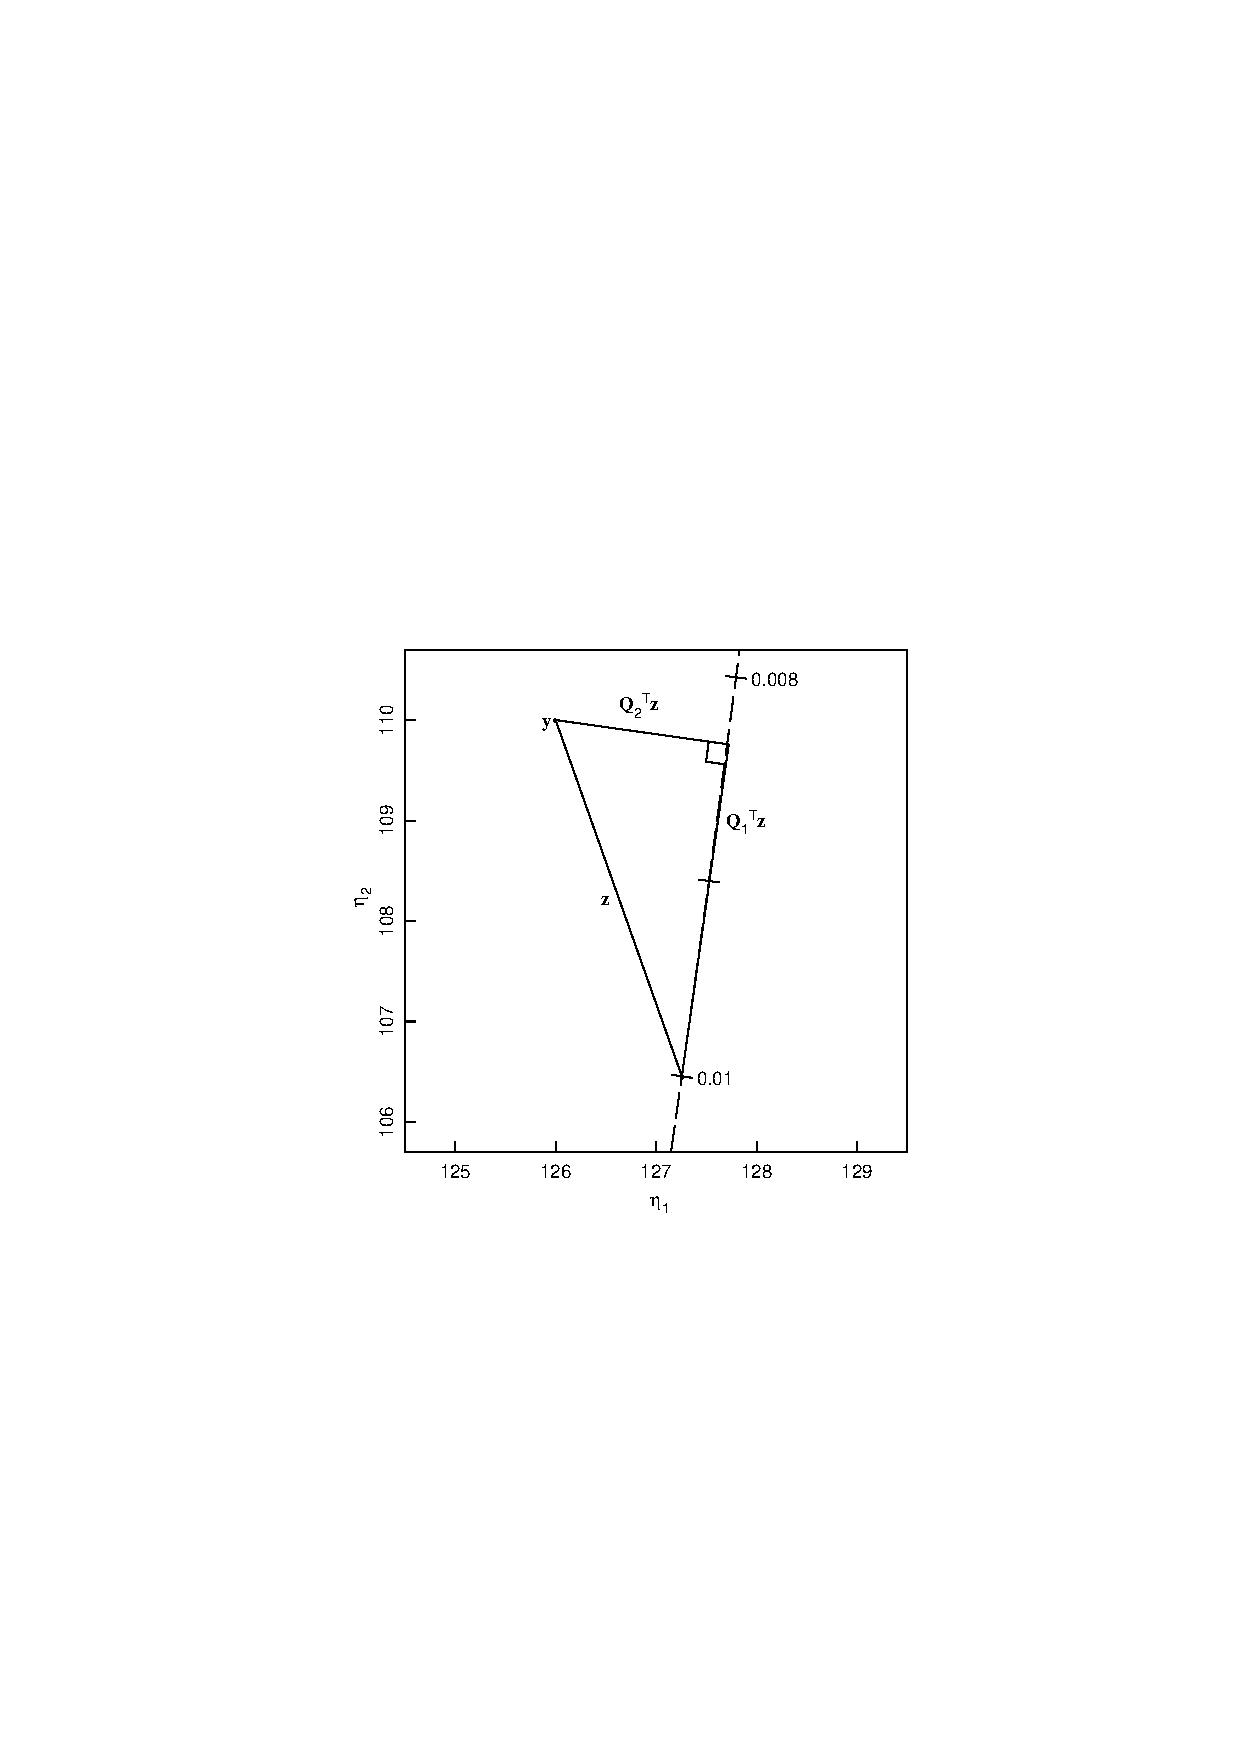
\includegraphics{2RUM2convge}}%,width=\textwidth}}
    \caption[Relative offset for the Rumford 2-case example]{
    \label{fig:RUM2convge}
    A geometric interpretation of relative offset using the 2-case
    Rumford data.
    A portion of the expectation surface (dashed line) is shown in
    the expectation space together with the residual vector $\bz$ and
    its projections into the tangent plane ($\bQ_1 \trans \bz$)
    and orthogonal to the tangent plane ($\bQ_2 \trans \bz$).
    }
  \end{figure}
Figure \ref{fig:RUM2convge} shows a portion of the expectation surface, the
observation point $\by$, and the tangent plane at
$\boeta ( 0.01 )$.
Also shown is the component of the residual vector in the tangent
plane, $\bQ_1 \trans \bz$, and the component orthogonal to
the tangent plane, $\bQ_2 \trans \bz$.
The tangent plane component is large relative to the orthogonal
component, having a relative offset of 1.92, and so we conclude
that the residual vector at $\theta = 0.01$ is not sufficiently
orthogonal for us to accept $\theta = 0.01$ as the converged
value.
\end{example}

Convergence implies that the best estimates of the
parameters have been obtained, under the assumption that the model is
adequate.
Before characterizing the precision of the
estimates using inference intervals or regions,
therefore, we should check the residuals for signs of model
inadequacy.
A complete discussion of the practical aspects of nonlinear
regression is given in Chapter 3, but in the interests of completeness
in analyzing the Puromycin and BOD data, we simply plot the residuals
versus the fitted values and using probability plots
before continuing.
\label{mic:resplots}
\begin{example}

Convergence for the Puromycin data was declared at
$\hat{ \btheta} = ( 212.7 ,  0.0641 ) \trans$, with $s^2= 119.5$
on 10 degrees of freedom.
Studentized residuals from the least squares fit are plotted in
Figure \ref{fig:PURresplots} versus
fitted values in part $a$ and as a normal probability plot in part $b$.
  \begin{figure}
    \centerline{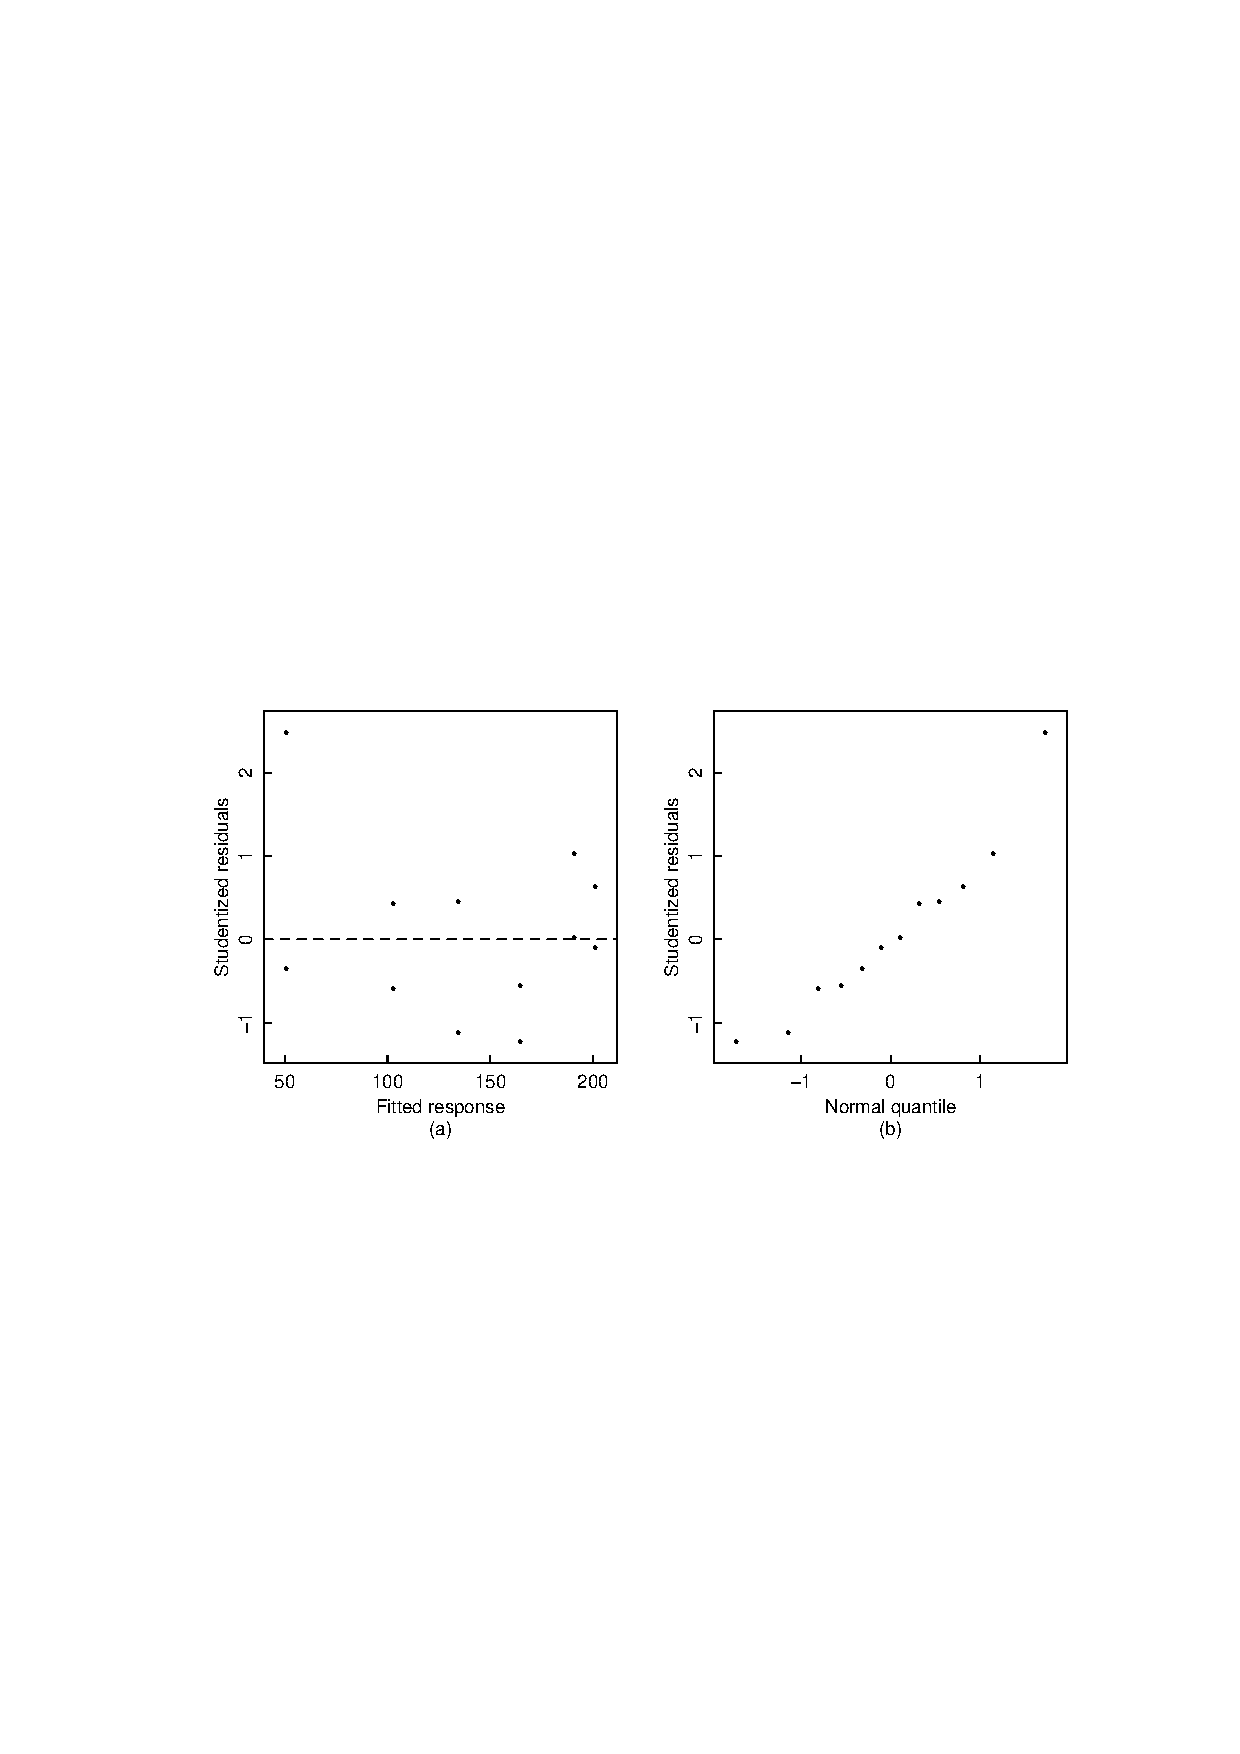
\includegraphics{2PURresplots}}%,width=\textwidth}}
    \caption[Studentized residuals for Puromycin data]{
    \label{fig:PURresplots}
    Studentized residuals for the Puromycin data plotted versus fitted values
    in part $a$ and versus normal quantiles in part $b$.
    }
  \end{figure}
Although there is one relatively large residual, the overall
fit appears adequate, and so we proceed to develop parameter
inference regions.
\end{example}
\begin{example}
\label{bod:resplots}

Convergence for the BOD data was declared at
$\hat{ \btheta} =( 19.143,  0.5311 ) \trans$, with $s^2=6.498$
on 4 degrees of freedom.
Studentized residuals from the least squares fit are plotted in
Figure \ref{fig:BODresplots} versus fitted values in part $a$ and as a
normal probability plot in part $b$.
  \begin{figure}
    \centerline{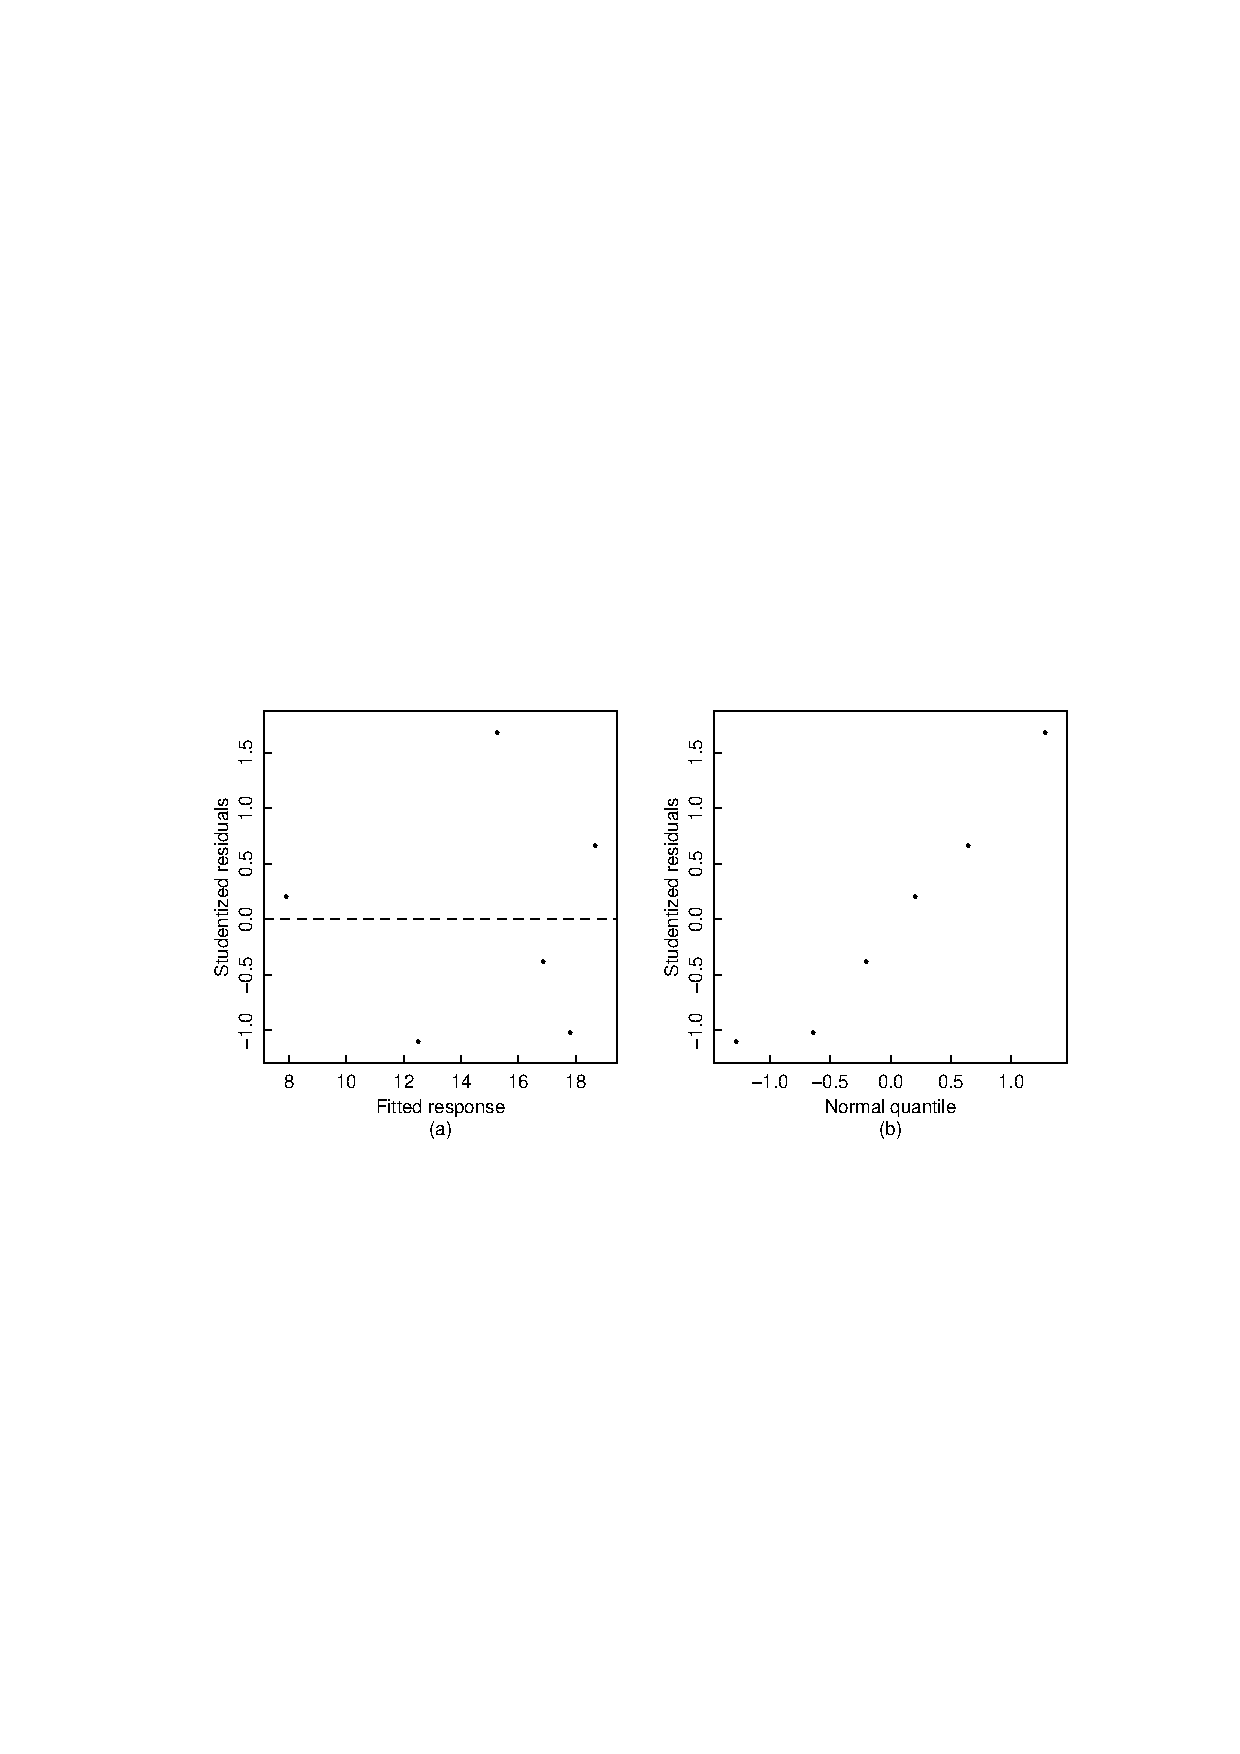
\includegraphics{2BODresplots}}%,width=\textwidth}}
    \caption[Studentized residuals for BOD data]{
    \label{fig:BODresplots}
    Studentized residuals for the BOD data plotted versus fitted values
    in part $a$ and versus normal quantiles in part $b$.
    }
  \end{figure}
Since the residuals are well behaved, we proceed to develop
parameter inference regions.
\end{example}

\section{Nonlinear Regression Inference Using the Linear Approximation}
\sectionmark{Inference Using Linear Approximation}

In the Gauss--Newton algorithm for calculating $\hat{ \btheta}$,
the derivative matrix $\bV$ is evaluated at each iteration and used
to calculate the increment and the convergence criterion.
It is natural, then, to apply the linear approximation to
\emph{inference} for nonlinear models with the derivative matrix
\index{inference!in nonlinear regression}
\index{inference!linear approximation}
evaluated at the least squares parameter estimates.
This yields approximate likelihood, confidence, or Bayesian
HPD regions, based on
  \begin{equation}\label{eqn:2.7a}
  \boeta ( \btheta ) = \boeta ( \hat{ \btheta} ) +
  \hat{ \bV} ( \btheta - \hat{ \btheta} )
  \end{equation}
\subsection{Approximate Inference Regions for Parameters 2 3 1}

Recall that in the linear case, a $1-\alpha$
parameter inference region can be expressed as [cf. (1.9)]
\index{parameter!inference region}
  \begin{equation}\label{eqn:infreg}
  ( \bbeta - \hat{ \bbeta} ) \trans \bX \trans \bX
  ( \bbeta - \hat{ \bbeta} )  \le  P s^2 \FPNP
  \end{equation}
Geometrically this region results because the expectation surface
is a plane and the residual vector is orthogonal to that plane,
so the region of plausible values on the expectation plane is a
disk.
Taking the disk through the linear mapping relating points on the
expectation plane to points on the parameter plane, then maps the
disk to an ellipsoid on the parameter plane.

Approximate inference regions for a nonlinear model are defined,
\index{parameter!approximate inference region}
by analogy with equation (\ref{eqn:infreg}), as
  \begin{equation}\label{eqn:linregion}
  ( \btheta - \hat{ \btheta} ) \trans \hat{ \bV} \trans \hat{ \bV}
  ( \btheta - \hat{ \btheta} ) 
  \le P s^2 \FPNP
  \end{equation}
or equivalently
  \begin{equation}\label{eqn:2.12}
  ( \btheta - \hat{ \btheta} ) \trans \hat{ \bR}_1 \trans \hat{ \bR}_1
  ( \btheta - \hat{ \btheta} ) 
  \le P s^2 \FPNP
  \end{equation}
where the derivative matrix $\hat{ \bV} = \hat{ \bQ}_1 \hat{ \bR}_1$
is evaluated at $\hat{ \btheta}$.
The boundary of this inference region (\ref{eqn:2.12}) is [cf. (1.28)]
  \begin{equation}\label{eqn:2.13a}
  \left\{\btheta = \hat{{\btheta}}+\sqrt{P s^2 \FPNP}\hat{{\bR}}_1^-1\bd
  |  \norm \bd \norm = 1 \right\}
  \end{equation}

Similarly, the approximate standard error for $\theta_p$ is $s$
times the
\index{parameter!approximate standard error}
\index{standard error!approximate}
length of the $p$th row of $\hat{ \bR}_1^-1$'-1p'
[cf. (1.33)].
Approximate correlations and standard errors for the parameters are easily
\index{parameter!approximate correlations}
calculated by factoring $\hat{ \bR}_{-1}$ into a
diagonal matrix [cf. (1.34)] giving the lengths of
the rows of $\hat{ \bR}^-1$ and a matrix with unit length rows
as described in Section 1.2.3.
The parameter approximate correlation matrix is calculated as in (1.35).
\label{mic:8}
\begin{example}

Convergence for the Puromycin data was declared at
$\hat{ \btheta} = ( 212.7 ,  0.0641 ) \trans$, with $s^2= 119.5$
on 10 degrees of freedom and
\begin{displaymath}
  \hat{ \bR}_1 =
  \begin{bmatrix}
    -2.4441 & 1568.7 \\
    0       & 1320.3 
  \end{bmatrix}
\end{displaymath}

The 95 and 99\% approximate joint inference regions were
obtained by evaluating (\ref{eqn:2.13a}) with
$\bd =( \cos\omega , \sin\omega ) \trans$ and are plotted in
Figure \ref{fig:MIClinregion}.
  \begin{figure}
    \centerline{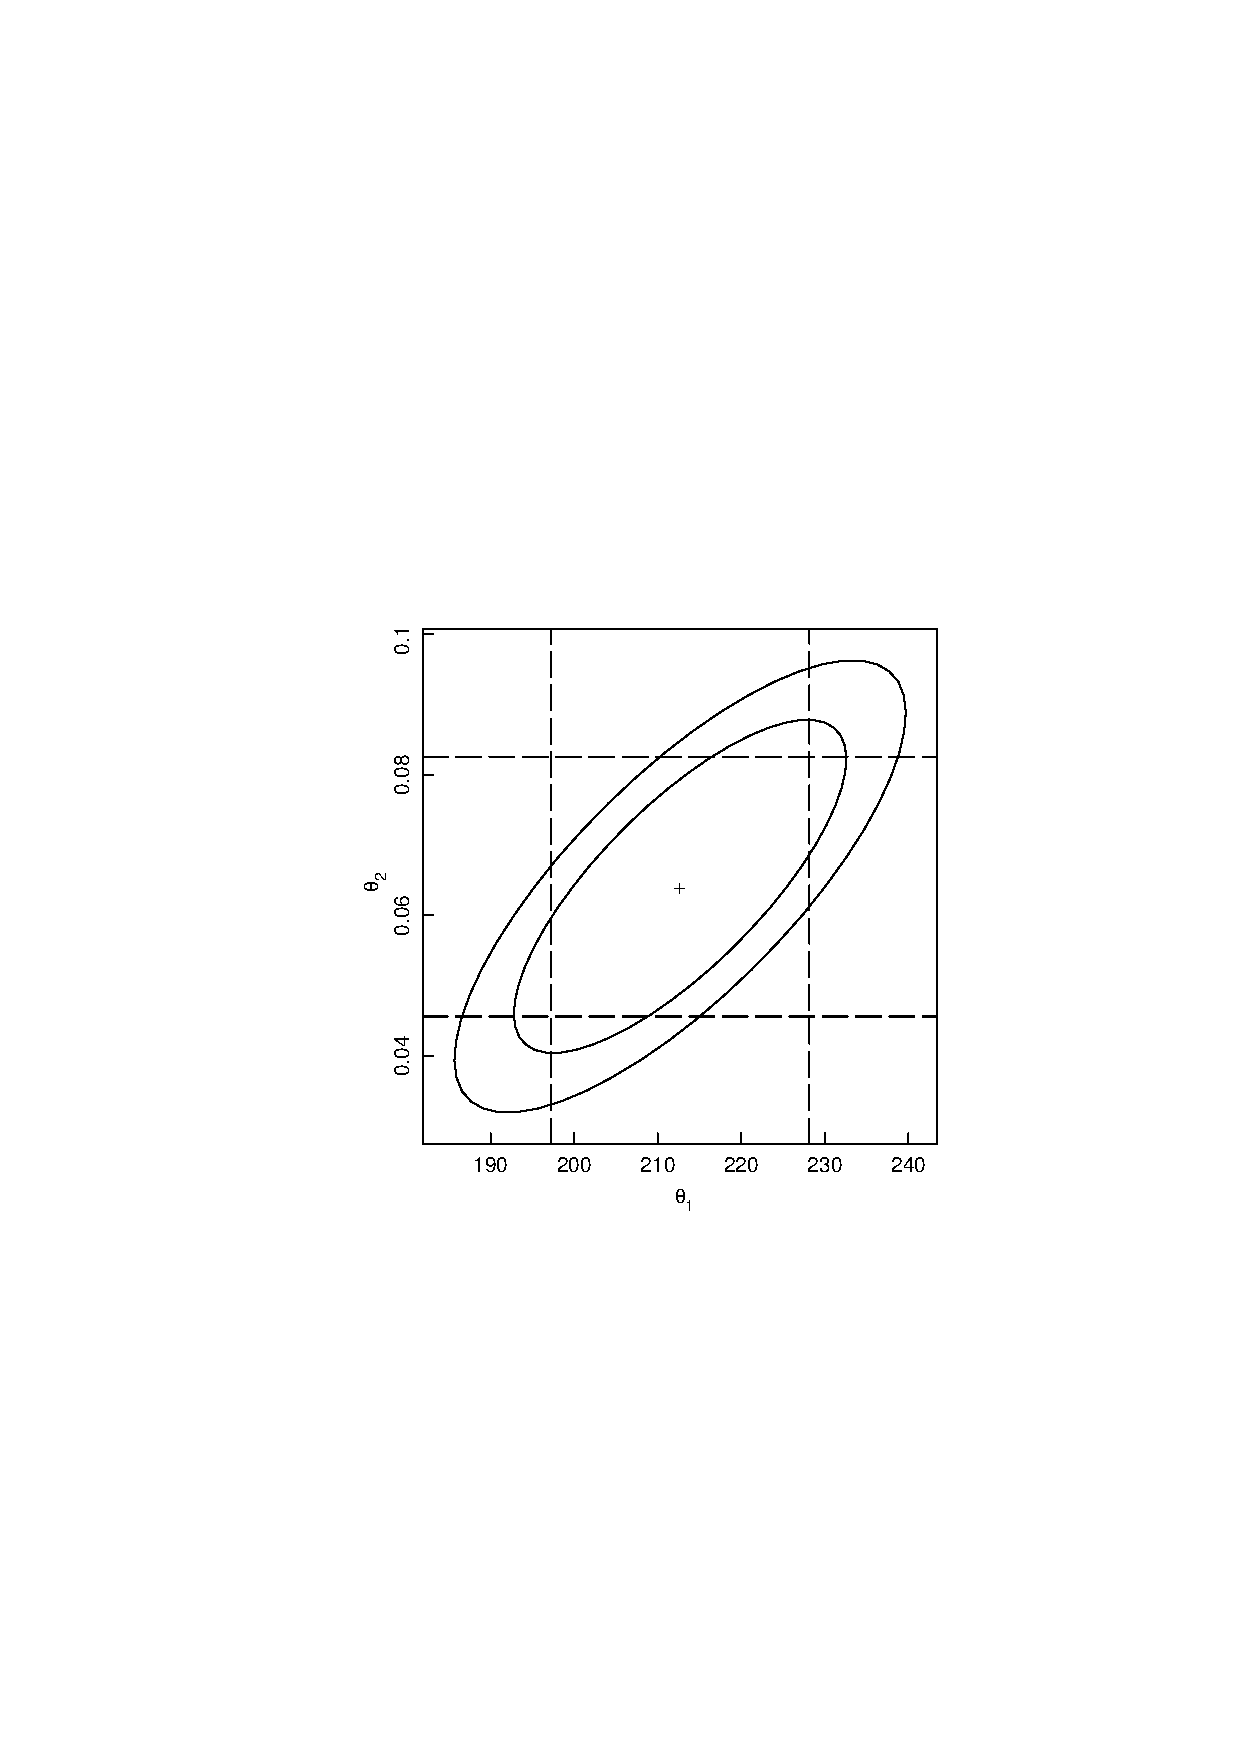
\includegraphics{2MIClinregion}}%,width=\textwidth}}
    \caption{\label{fig:MIClinregion}
    Parameter approximate inference regions for the Puromycin data.
    We show the least squares estimates ($+$),
    the parameter joint 95 and 99\% inference regions (solid lines),
    and the marginal 95\% inference intervals (dashed lines).
    }
  \end{figure}
To calculate approximate marginal inference intervals, we factor
\begin{eqnarray*}
  \hat{ \bR}_1^{-1}&=&
  \begin{bmatrix}
    -0.4092 & 0.4861\\
    0      & 0.0007574
  \end{bmatrix}\\
  &=&\begin{bmatrix}0.6354&0\\0&0.0007574\end{bmatrix}
  \begin{bmatrix}
    -0.6439 & 0.7651\\
    0       & 1.0000
  \end{bmatrix}
\end{eqnarray*}
so the approximate standard errors are 6.95 and
$8.28 \times10^-3$ and the approximate correlation between
$\theta_1$ and $\theta_2$ is 0.77.
A 95\% approximate marginal inference interval for $\theta_2$, for
example, is
  \begin{displaymath}
    0.0641  \pm { \sqrt 119.5 }  (0.0007574)  t ( 10 ;  0.025 )
  \end{displaymath}
or $0.0641 \pm 0.0185$.
The 95\% marginal inference intervals for both parameters are shown as
dashed lines in Figure
\ref{fig:MIClinregion}.
\end{example}

\begin{example}\label{bod:2}
Convergence for the BOD data was declared at
$\hat{ \btheta} =( 19.143,  0.5311 ) \trans$, with $s^2 = 6.498$
on 4 degrees of freedom and
\begin{displaymath}
  \hat{ \bR}_1 =
  \begin{bmatrix}
    -1.9556 & -20.4986\\
    0 & -12.5523
  \end{bmatrix}
\end{displaymath}
giving approximate standard errors of 2.50 and 0.203.

The 95 and 99\% approximate joint inference regions are plotted in
Figure \ref{fig:BODlinregion} together with the 95\% approximate
marginal intervals.
Note that the regions include negative values for $\theta_2$, and such
values are not physically meaningful.
  \begin{figure}
    \centerline{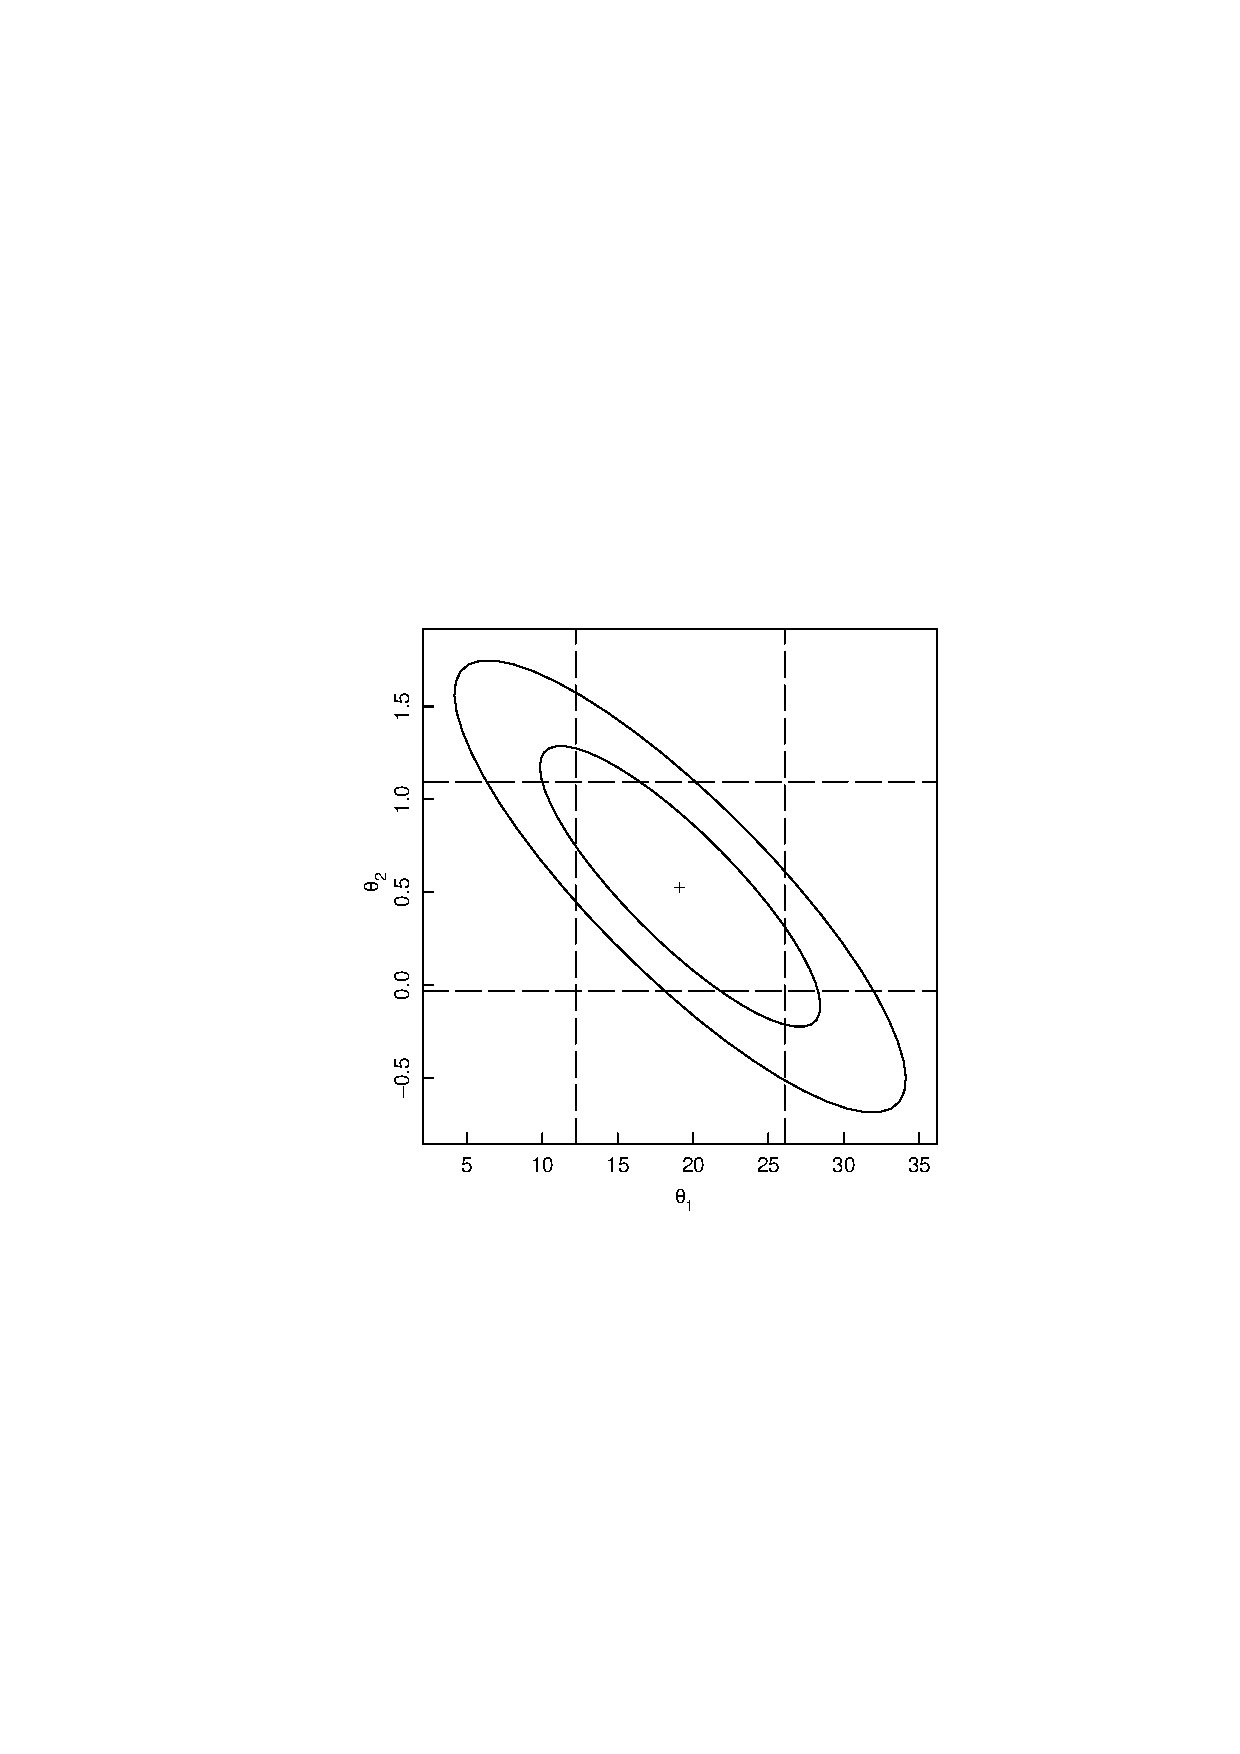
\includegraphics{2BODlinregion}}%,width=\textwidth}}
    \caption{\label{fig:BODlinregion}
    Parameter approximate inference regions for the BOD data.
    We show the least squares estimates ($+$),
    the parameter joint 95 and 99\% inference regions (solid lines),
    and the marginal 95\% inference intervals (dashed lines).
    }
  \end{figure}
The approximate correlation between $\theta_1$ and
$\theta_2$ is $-0.85$.
\end{example}

When there are more than two parameters, it is not possible to plot
the joint approximate inference region, and so it is common to
summarize the inferential situation by quoting the approximate
marginal inference intervals and the parameter correlation matrix and
by making
\index{parameter!correlation matrix}
\index{matrix!parameter correlation}
pairwise plots of the inference region.
More exact methods for summarizing the inferential situtation are
presented in Chapter 6.
\label{iso:1}
\begin{example}

Data on the reaction rate of the catalytic isomerization of
$n$-pentane to isopentane versus the partial pressures of hydrogen,
$n$-pentane, and isopentane as given in
\citeasnoun{carr:1960}%\glossary{ Carr, N.L.} are presented in
Appendix A, Section~\ref{atbl:iso}, and plotted in Figure \ref{fig:ISOdata}.
  \begin{figure}
    \centerline{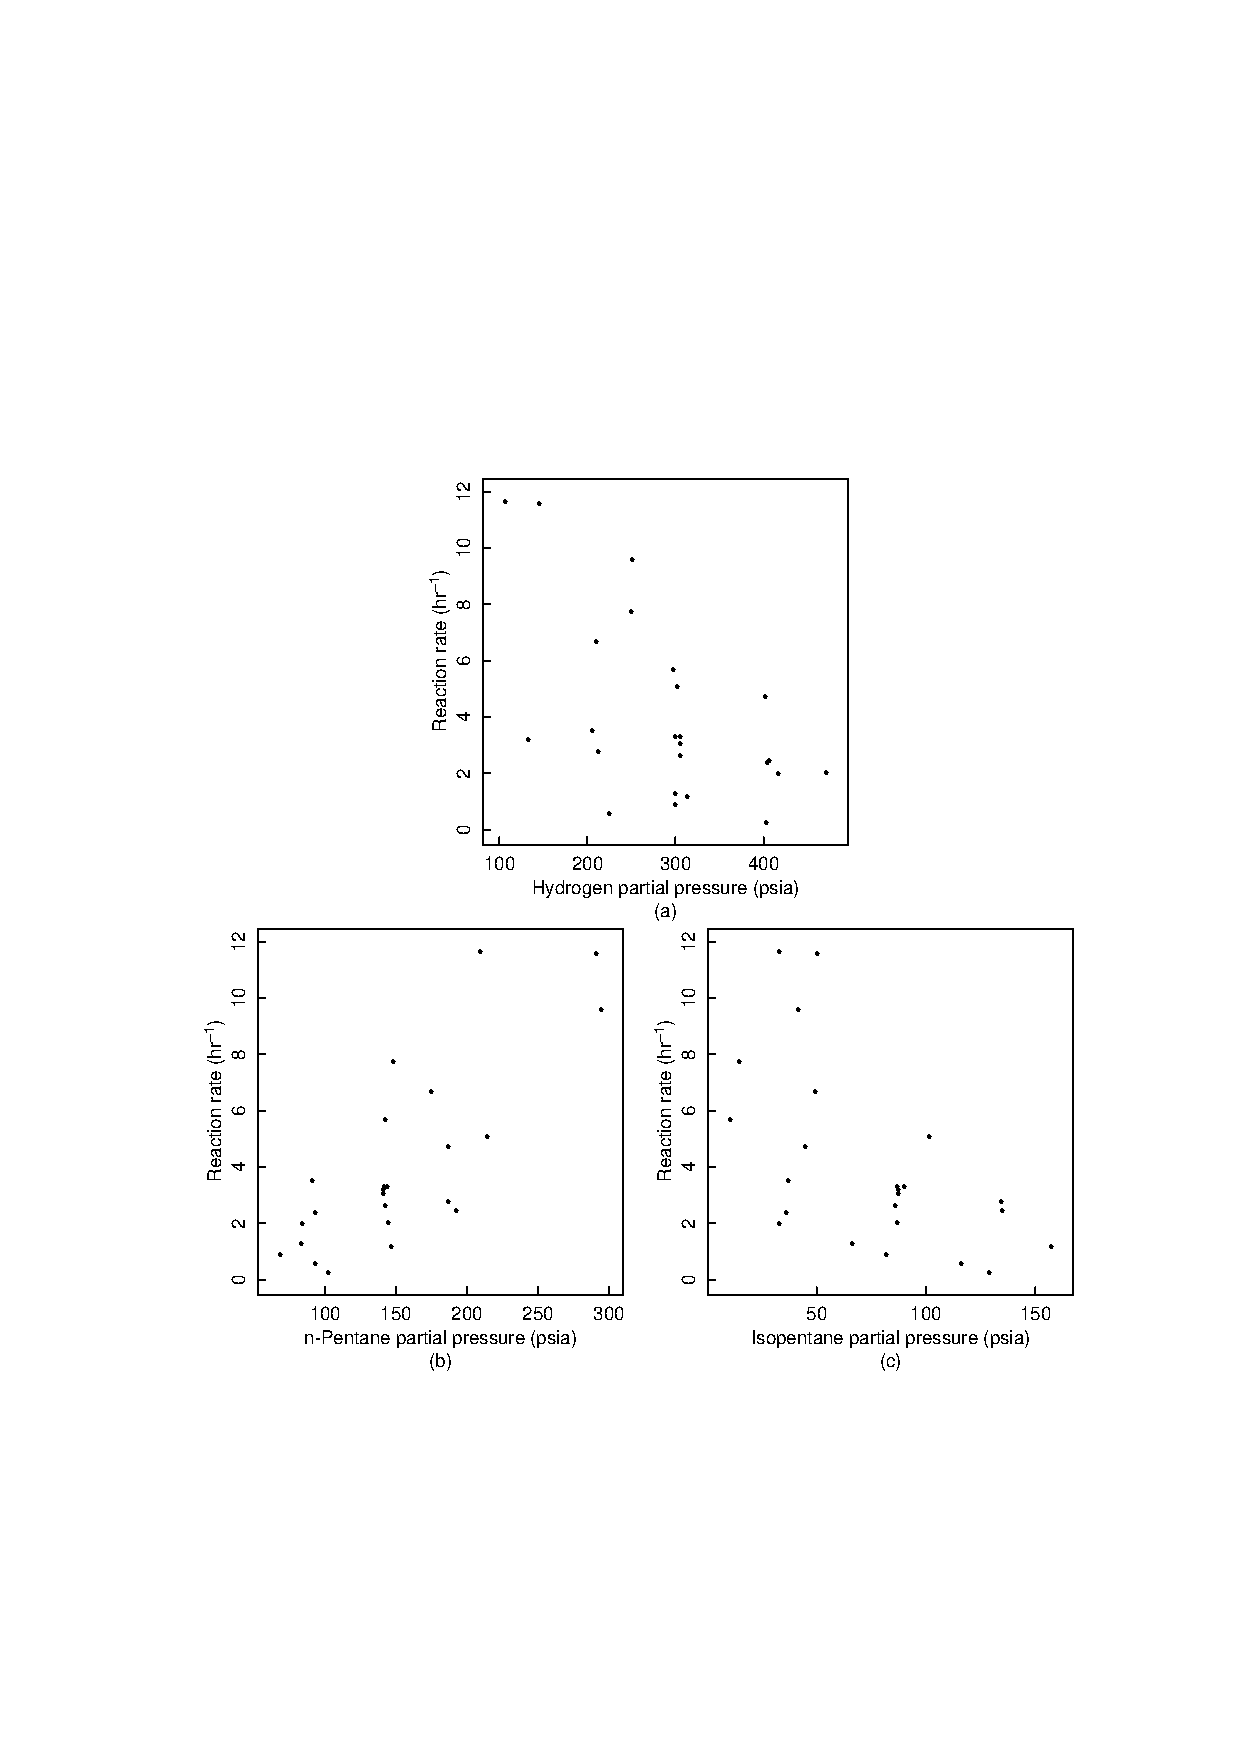
\includegraphics{2ISOdata}}%,width=\textwidth}}
    \caption{\label{fig:ISOdata}
    Plots of reaction rate of the isomerization of
    $n$-pentane to isopentane versus the partial pressures of
    hydrogen in part $a$, $n$-pentane in part $b$, and isopentane in part
    $c$.
    }
  \end{figure}
A proposed model function for these data is
  \begin{equation}\label{eqn:2.9a}
  f ( \bx , \btheta ) =
  \frac{\theta_1 \theta_3 ( x_2 - x_3 / 1.632 )}{1 + \theta_2 x_1 +
  \theta_3 x_2 + \theta_4 x_3} 
  \end{equation}
Parameter estimates and summary statistics are given in
Table \ref{tbl:isoest}, and residual plots versus the partial pressures and
  \begin{table}
%c c c c s s s
%l c c c s s s
%c c c c s s s
%c n n n 1 n 1 n 1 n.
%\_
%:::Approximate
%Parameter:Estimate:Standard:Correlation
%::Error:Matrix
%\par\vspace{2.0pt}
%\_
%$\theta_1$:35.92:8.21:1.000
%$\theta_2$:0.0708:0.1783:--\/0.805:1.000
%$\theta_3$:0.0377:0.0998:--\/0.840:0.998:1.000
%$\theta_4$:0.167:0.415:--\/0.790:0.998:0.995:1.000
%\par\vspace{4.0pt}
%\_
    \vspace{1in}
    \caption{\label{tbl:isoest}
    Parameter summary for the isomerization data}
  \end{table}
the fitted values in Figure \ref{fig:ISOresplots}.
The plots show the residuals are generally well behaved.
The summary statistics suggest potential difficulties, since
some of the correlations are extremely high and some of the standard
errors produce approximate 95\% intervals which include negative
values, but the parameters must be positive to be physically meaningful.
  \begin{figure}
    \centerline{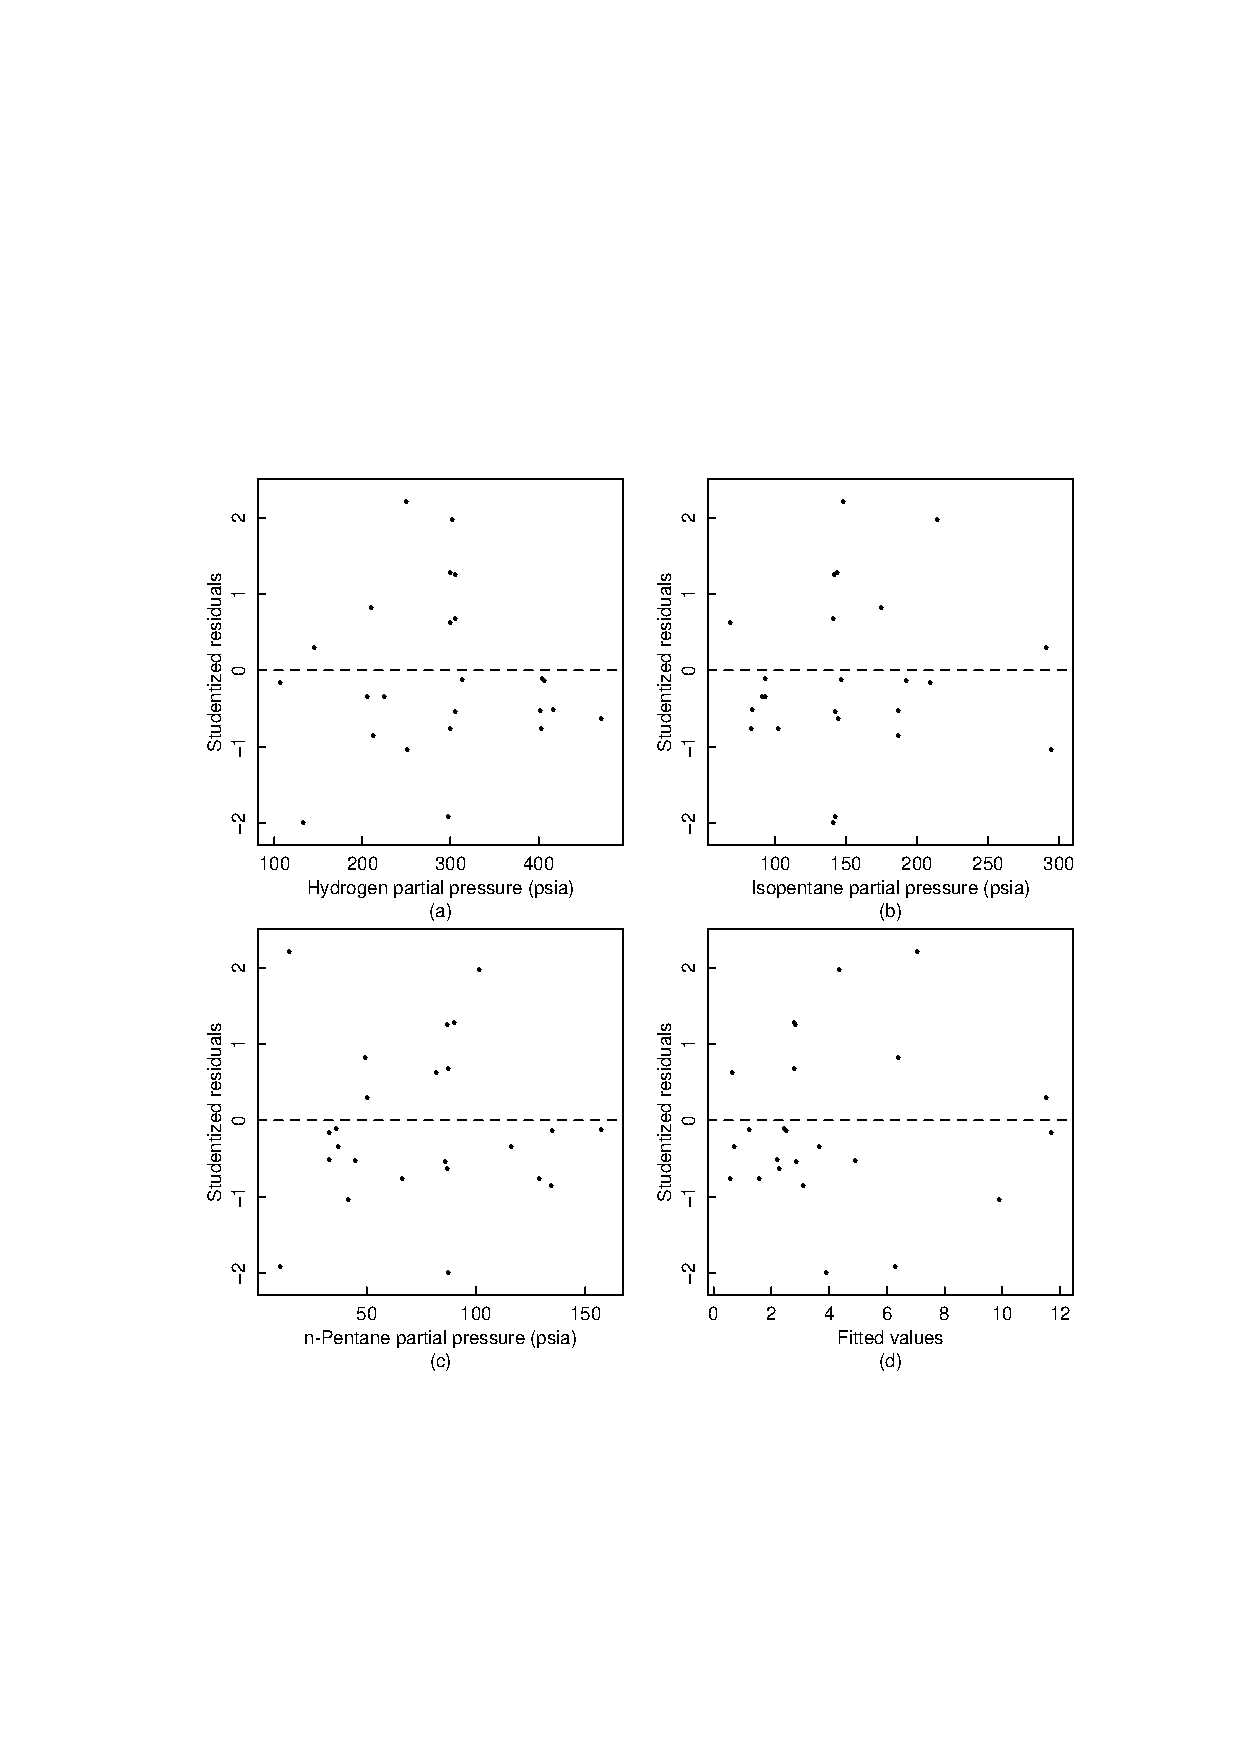
\includegraphics{2ISOresplots}}%,width=\textwidth}}
    \caption{\label{fig:ISOresplots}
    Studentized residuals for the isomerization data are plotted
    versus the partial pressures of hydrogen in part $a$, isopentane in
    part $b$, and $n$-pentane in part $c$, and versus the
    fitted values in part $d$.
    }
  \end{figure}
The pairwise plots of the parameter approximate 95\% inference
region, given in Figure \ref{fig:ISOlinregion},
  \begin{figure}
    \centerline{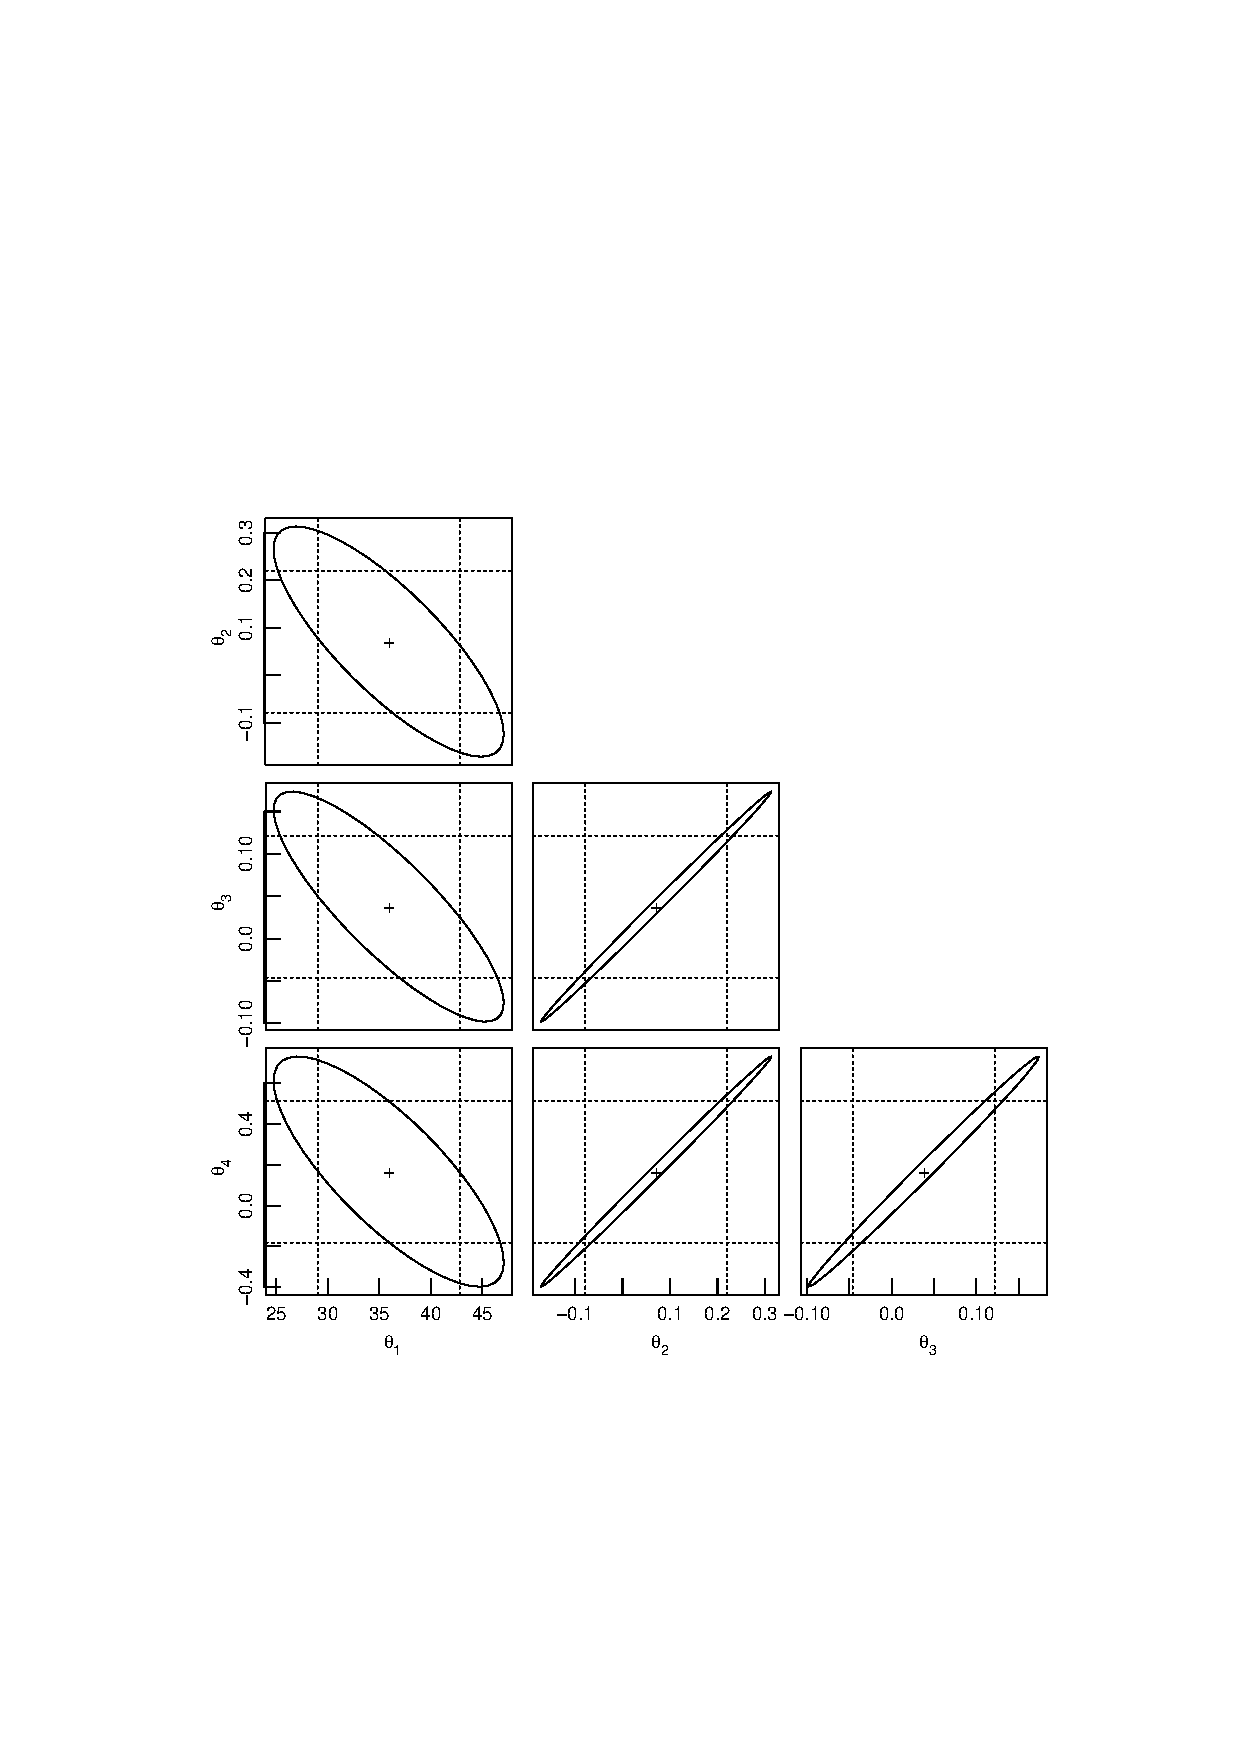
\includegraphics{2ISOlinregion}}%,width=\textwidth}}
    \caption{\label{fig:ISOlinregion}
    Pairwise plots of the parameter approximate 95\% inference region for
    the isomerization data.
    For each pair of parameters we show the least squares estimates ($+$),
    the parameter approximate joint 95\% inference region (solid line),
    and the approximate marginal 95\% inference intervals (dotted lines).
    }
  \end{figure}
clearly extend into negative parameter regions.
\end{example}

\subsection{Approximate Inference Bands for the Expected Response}

Linear approximation inference intervals and bands
\index{linear approximation!inference interval}
\index{inference!interval, linear approximation}
\index{linear approximation!inference band}
\index{inference!band, linear approximation}
for the expected response
in nonlinear regression can be generated using the analogs of the
equation for linear regression, (1.11) and (1.12).
In those equations, we simply
replace the estimated value $\bx_0 \trans \hat{ \bbeta}$ by
$f ( \bx_0 , \hat{ \btheta} )$, the matrix $\bX$ by $\hat{ \bV}$,
and the derivative vector $\bx_0$ by
\index{derivative!vector}
  \begin{displaymath}
    \bv_0=\left.\frac{\partial f ( \bx_0 , \btheta )}{\partial
    \btheta \trans }\right|_{\hat{ {\theta}}}
  \end{displaymath}
The $1 - \alpha $ approximate inference interval is then
  \begin{displaymath}
    f( \bx_0 , \hat{ \btheta} ) \pm s \norm \bv_0 \trans \hat{
    \bR}_1^{-1}\norm\tNP\quad\mbox{\rm [cf.(1.36)]}
  \end{displaymath}
and the $1-\alpha$ approximate inference band is
  \begin{displaymath}
    f( \bx  , \hat{ \btheta} ) \pm s \norm \bv  \trans \hat{ \bR}_1^{-1}
    \norm \sqrt{P\FPNP}\quad\mbox{\rm [cf.(1.37)]}
  \end{displaymath}

\begin{example}\label{mic:9}

For the Puromycin data, the estimated response at
$x  = 0.4$ is 183.3 and the derivative vector is
$\bv = ( 0.8618 ,  -394.9 ) \trans$, so that,
using $\hat{ \bR}_1^{-1}$ from Example Puromycin 6,
$ \bv \trans \hat{ \bR}_1^{-1}  = ( -0.3526,0.1198 )$.
The inference band at $x = 0.4$ is then
$(171.6,195.0)$.
A plot of the approximate 95\% inference band is given in
Figure \ref{fig:MICband}.
The band gradually widens from zero width at $x=0$ to a constant
width as $x\to\infty$.
  \begin{figure}
    \centerline{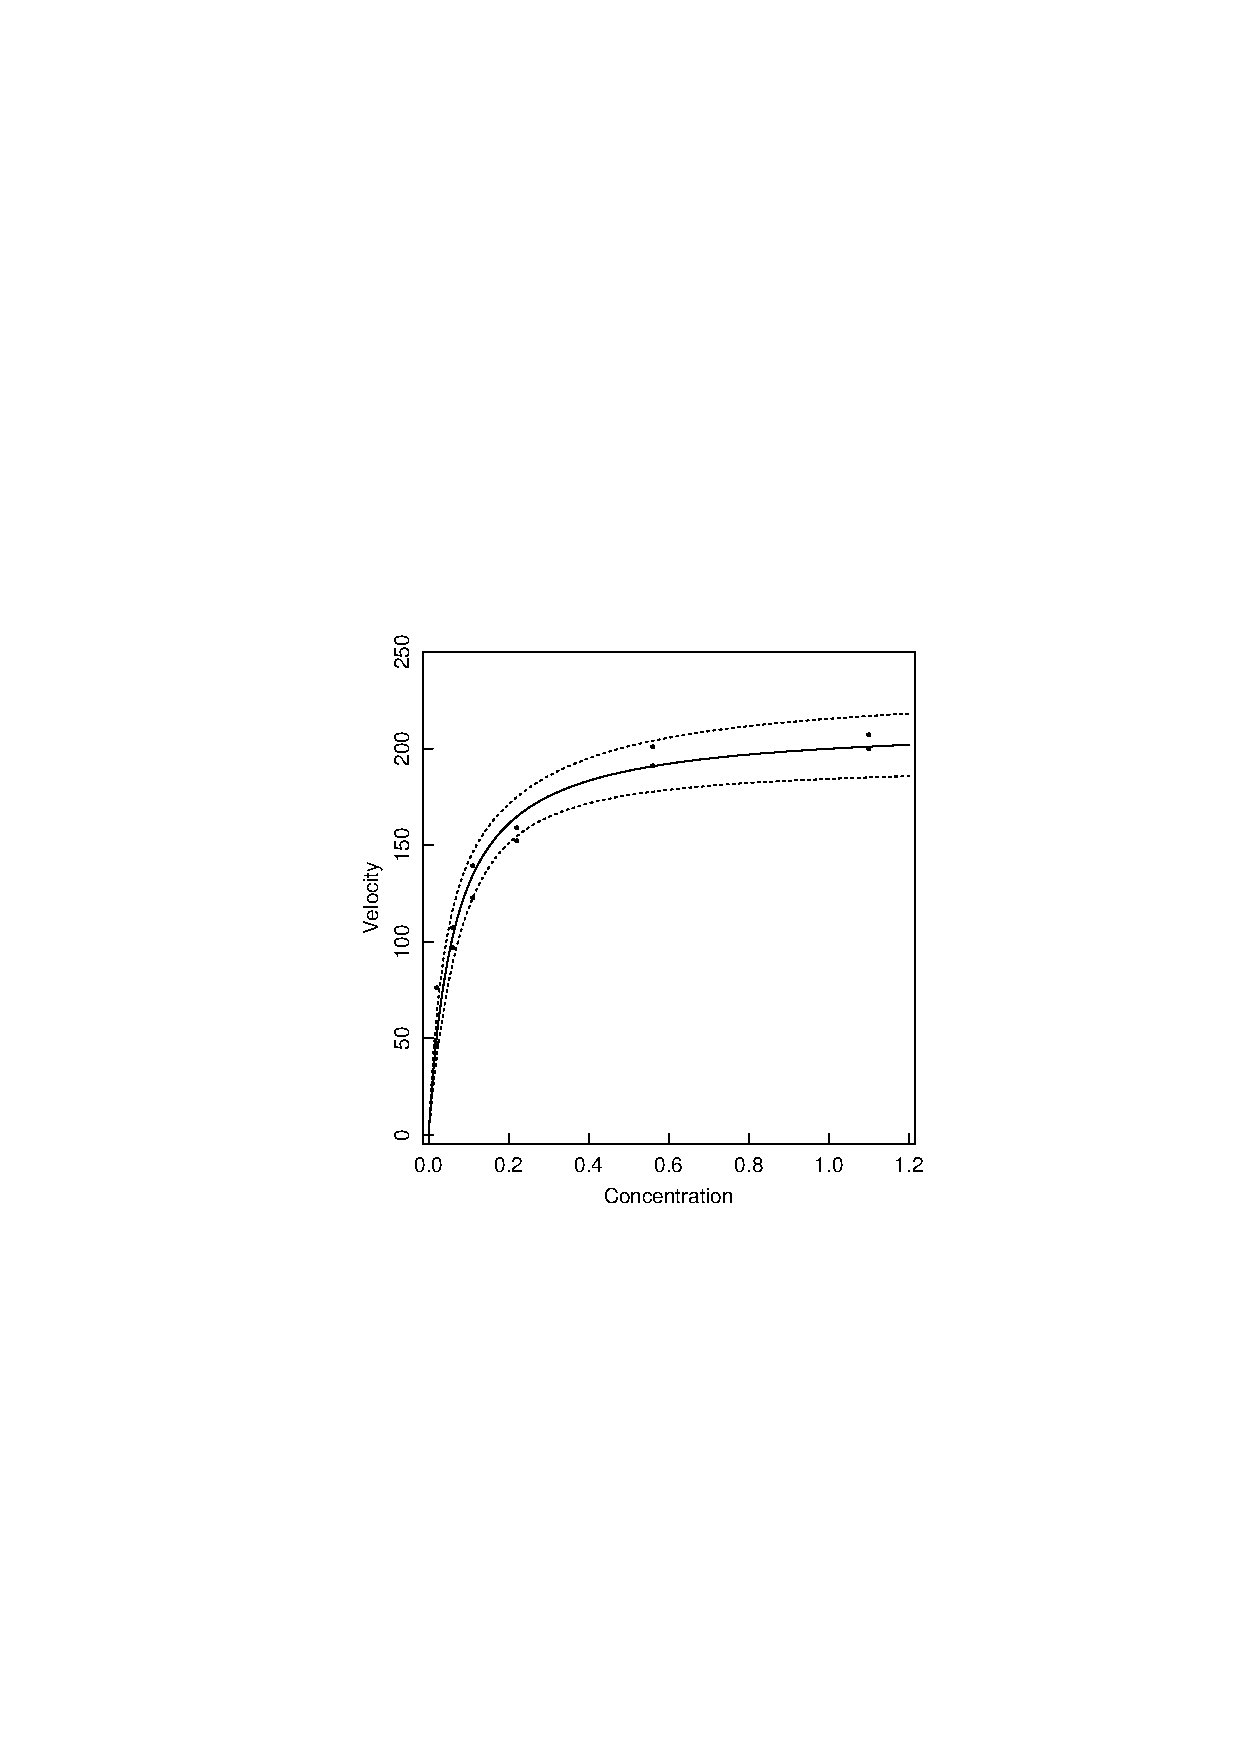
\includegraphics{2MICband}}%,width=\textwidth}}
    \caption{\label{fig:MICband}
    Approximate 95\% inference band for the Puromycin data.
    The fitted expectation function is shown as a solid line, and the 95\%
    inference band is shown as a pair of dotted lines.
    }
  \end{figure}
\end{example}

\begin{example}\label{bod:3}

The estimated response function for the BOD data
and the approximate 95\% inference band is plotted in
Figure \ref{fig:BODband}.
  \begin{figure}
    \centerline{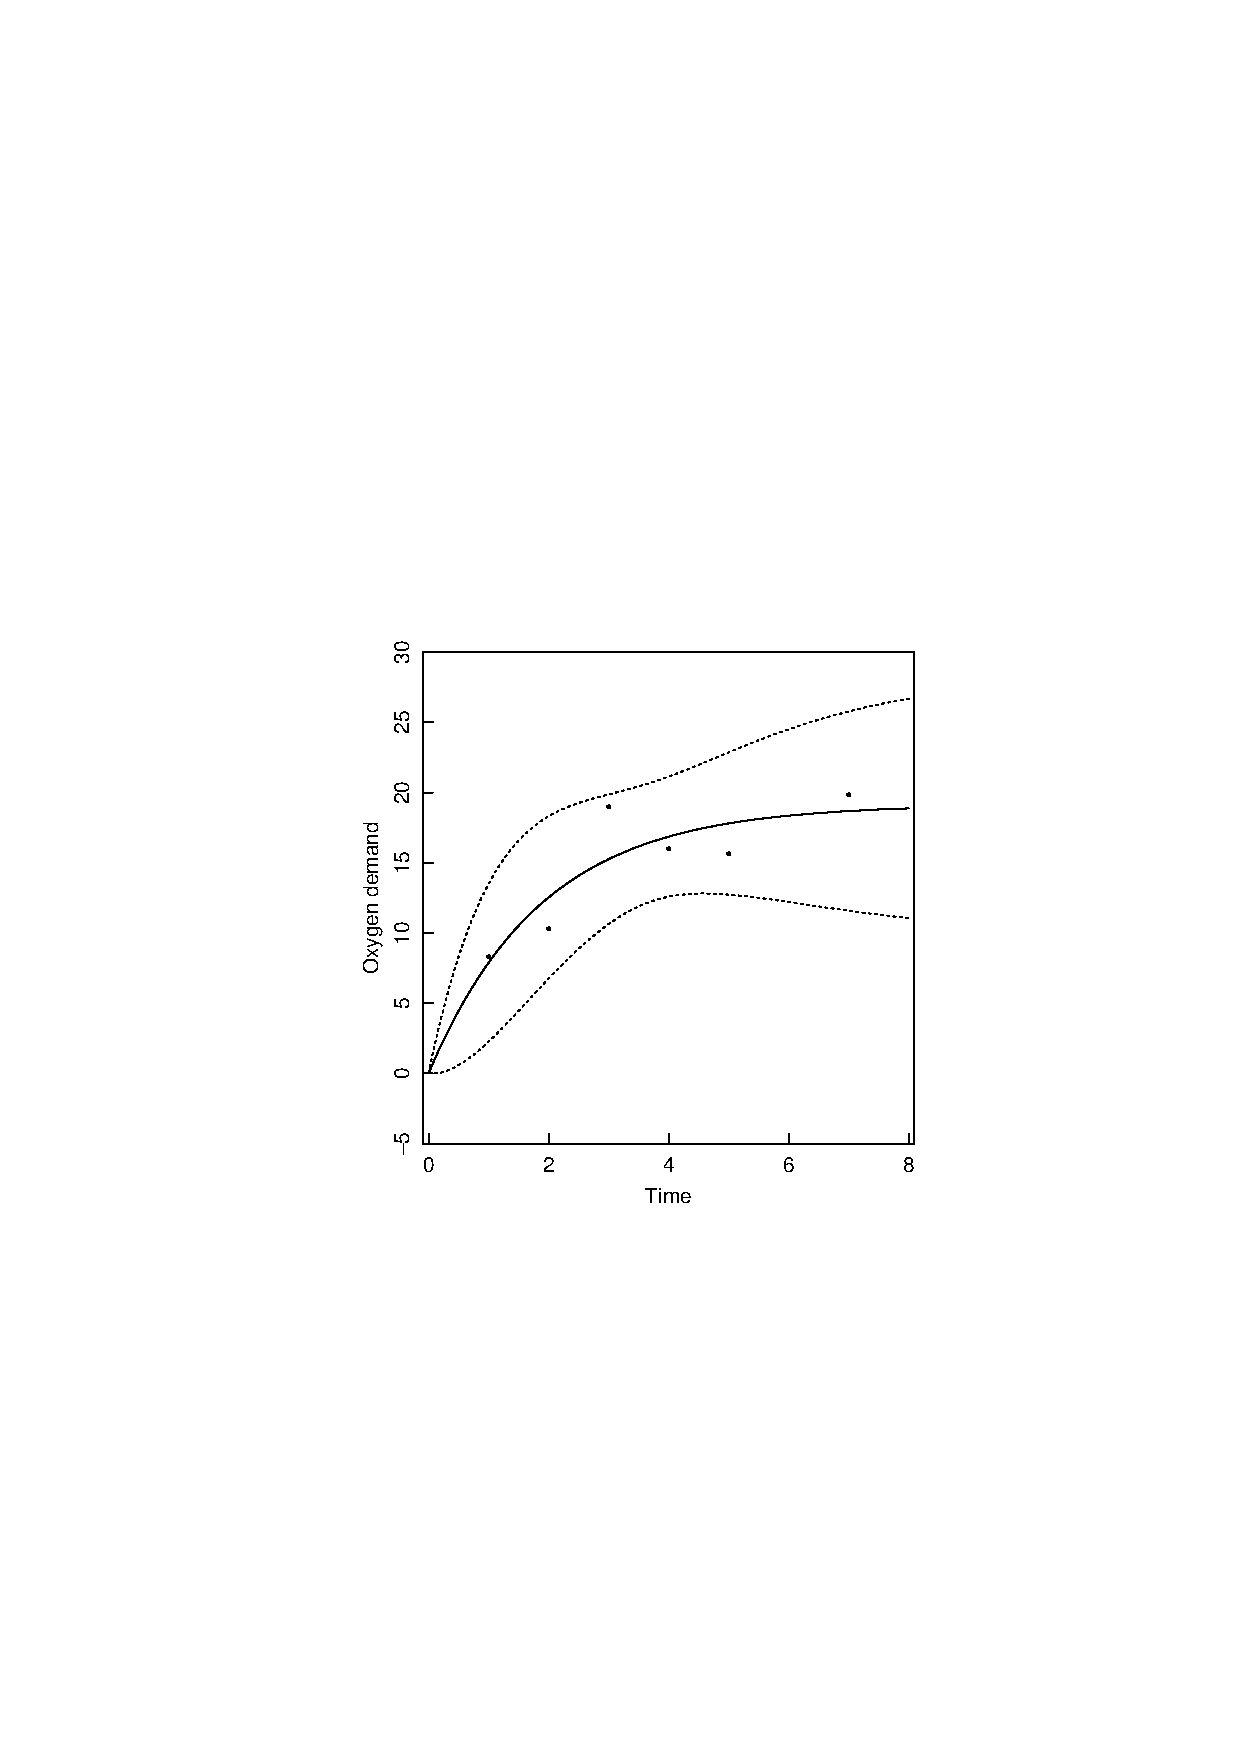
\includegraphics{2BODband}}%,width=\textwidth}}
    \caption{\label{fig:BODband}
    Approximate 95\% inference band for the BOD data.
    The fitted expectation function is shown as a solid line, and the 95\%
    inference band is shown as a pair of dotted lines.
    }
  \end{figure}
The band widens from zero width at $x=0$, narrows around $x=4$ and
then gradually approaches a constant width as $x\to\infty$.
\end{example}

Inference bands for nonlinear models behave quite
differently from those for linear models.
In the above examples,
because the functions are constrained to go through the
origin, the bands reduce to 0 there.
Also, because the model functions approach horizontal asymptotes,
the inference bands approach asymptotes.
These characteristics differ from those of the inference bands
for linear models as exemplified in Figure 1.3.
There it is seen that the bands are narrowest near the middle of
the data, and expand without limit.

\section{Nonlinear Least Squares via Sums of Squares}
\index{nonlinear!least squares via sums of squares}

Sums of squares occur explicitly in linear and nonlinear least
squares because of the assumptions of normality, independence,
and constant variance of the disturbances.
It is therefore natural to view linear and nonlinear regression
via sums of squares, which can help in understanding these two
topics.
The likelihood approach is especially closely linked to sum of
\index{likelihood}
squares contours, because the loglikelihood function is directly
\index{loglikelihood!function}
proportional to the sum of squares function $S ( \btheta )$.
\index{sum of squares!function}

An important characteristic of linear models is that the sum of
squares function $S ( \bbeta $) is quadratic.
Because of this, contours of constant sums of squares are
well-behaved regular curves or surfaces, such as ellipses and
ellipsoids, and so the loglikelihood function can be completely
summarized by:
  \begin{itemize}
    \item the minimum value of the sum of squares function,
          $S ( \hat{\bbeta} )$,
    \item the location of the minimum of the sum of squares function,
          $ \hat{\bbeta} $, and 
    \item the second derivative (Hessian) of the sum of squares
          \index{ Hessian "of sum of squares function"}
          function,
          \begin{displaymath}
            \frac{\partial^2 S ( \bbeta )}{\partial \bbeta \partial \bbeta
            \trans}= \bX \trans \bX    
          \end{displaymath}
  \end{itemize}
Furthermore, all these quantities can be
determined analytically.
For nonlinear models, however, the sum of squares function is not
regular or well behaved, and so it is difficult to summarize the
loglikelihood function.
\subsection{The Linear Approximation}
\index{linear approximation!to sum of squares function}

Linear approximations of the expectation function are used to
determine increments while seeking the least squares estimates,
and to determine approximate inference regions when convergence
has been achieved.
The linear approximation to $\boeta ( \btheta )$ based at $\btheta^0$,
(\ref{eqn:2.5}), produces a linear approximation to the
residual vector $\bz ( \btheta )$, (\ref{eqn:2.5a}), and hence a
\emph{quadratic} approximation $ \tilde S ( \btheta )$ to the sum of
squares function $S(\btheta)$, since
  \begin{eqnarray}\label{eqn:quada}
        S(\btheta)&=&\norm \by - \boeta ( \btheta ) \norm^2\\
        &=&\bz ( \btheta ) \trans  \bz ( \btheta )  \approx
        \tilde S(\btheta)\nonumber\\
        &=&[\bz^0-\bV^0(\btheta-\btheta^0)]\trans
        [\bz^0-\bV^0(\btheta-\btheta^0)]\nonumber\\
        &=&{\bz^0}\trans\bz^0-2{ \bz^0 } \trans \bV^0 ( \btheta -
        \btheta^0 ) + ( \btheta - \btheta^0 ) \trans { \bV^0 } \trans
        \bV^0 ( \btheta - \btheta^0 )\nonumber\\
        &=&S(\btheta^0)-2[\by-\boeta(\btheta^0)]\trans \bV^0
        ( \btheta - \btheta^0 )
        + ( \btheta - \btheta^0 ) \trans { \bV^0 } \trans \bV^0
        ( \btheta - \btheta^0 )
  \end{eqnarray}
The location of the minimum of $\tilde S ( \btheta )$ is
  \begin{displaymath}
    \btheta^1 = \btheta^0 +
( {\bV^0} \trans \bV^0 )^-1 { \bV^0 } \trans \bz^0
  \end{displaymath}
which gives the Gauss--Newton increment.

Note that the quadratic approximation (\ref{eqn:quada}) is
not the second order Taylor series approximation to $S ( \btheta )$
based at $\btheta^0$.
The Hessian in the Taylor series approximation includes
a term involving the second order partial derivatives of the
model function with respect to the parameters (see Section 3.5.1).

Contours of the approximate sum of squares function
\index{sum of squares!contour}
\index{contour!sum of squares}
(\ref{eqn:quada}) are ellipsoids centered at $\btheta^1$ and of
the form
  \begin{displaymath}
    ( \btheta - \btheta^1 ) \trans { \bV^0 } \trans \bV^0
( \btheta - \btheta^1 ) = c
  \end{displaymath}
Of particular interest is the approximating contour
  \begin{displaymath}
    ( \btheta - \btheta^1 ) \trans { \bV^0 } \trans \bV^0
( \btheta - \btheta^1 ) = {\bz^0} \trans
\bV^0 ( {\bV^0} \trans \bV^0 )^{-1} {\bV^0} \trans \bz^0
  \end{displaymath}
which passes through $\btheta^0$.
If this contour is close to the actual sum of squares contour
which passes through $\btheta^0$, then we can expect that
$\btheta^1$ will be close to the optimal value of $\btheta$.
\label{rum:sumsq}
\begin{example}
  \begin{figure}
    \centerline{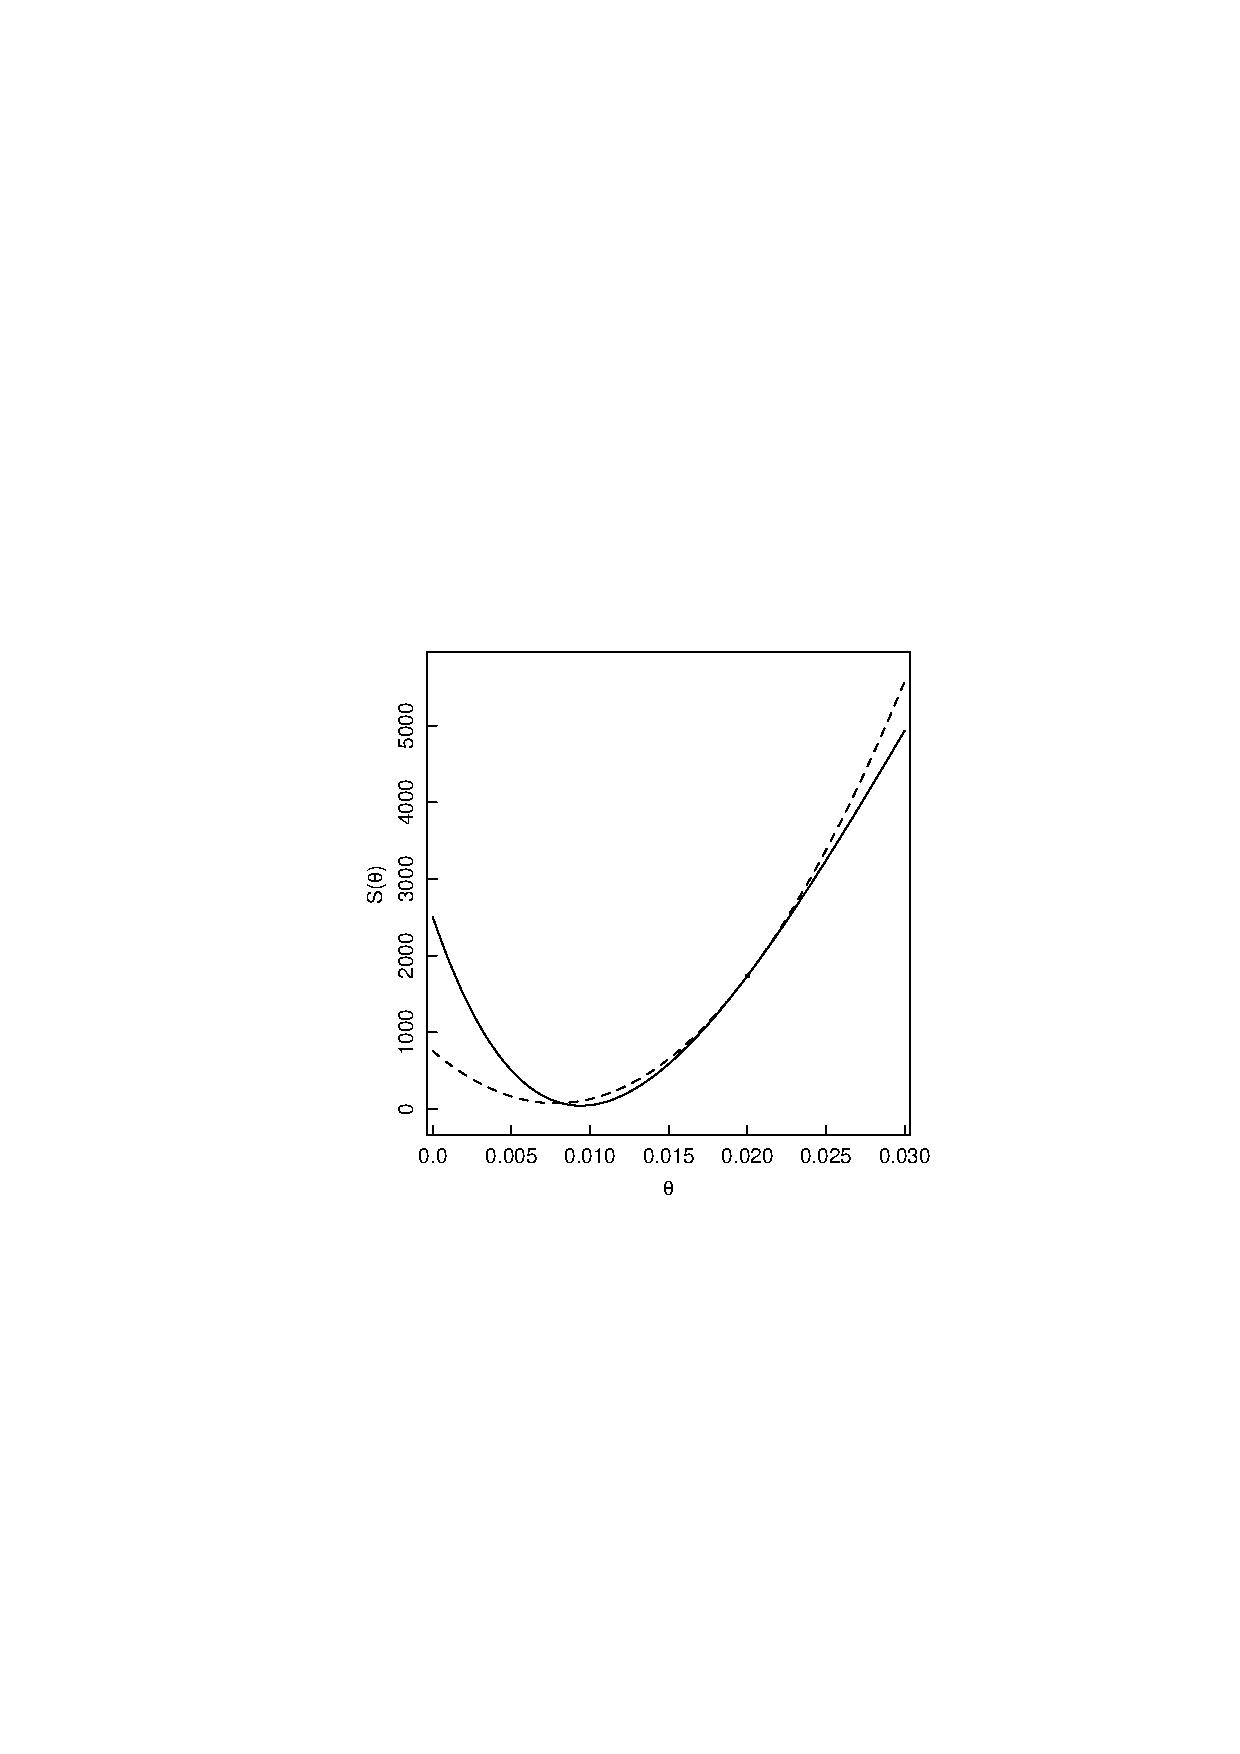
\includegraphics{2RUMsumsq}}%,width=\textwidth}}
    \caption[Sum of squares function for the Rumford data.]{
    \label{fig:RUMsumsq}
    Sum of squares function for the Rumford data.
    The true sum of squares curve is shown as a solid line, and the
    parabola from the linear approximation at $\theta^0=0.02$ is
    shown as a dashed line.
    }
  \end{figure}
In Figure \ref{fig:RUMsumsq} we plot the sum of squares function,
$S ( \theta )$, for the Rumford data as a solid line.
Superimposed on the plot is the approximating quadratic,
$\tilde S ( \theta )$, obtained by taking a linear Taylor
series approximation to the expectation function at
$\theta^0 = 0.02$, shown as a dashed line.

A careful examination of $S ( \theta )$ shows that it is not a parabola
but is asymmetric, with a steeper rise to the left of the
minimum than to the right.
The closeness of $S ( \theta )$ to a parabola indicates the small
degree of nonlinearity of this model--data set combination.
\index{nonlinearity!of model-data set}
The minimum of the approximating parabola is at
0.008, and so the Gauss--Newton increment is $0.008-0.02=-0.012$.
\end{example}
\label{mic:micSinc}
\begin{example}

In Figure \ref{fig:MICsumsqinc} we plot sum of squares contours,
  \begin{figure}
    \centerline{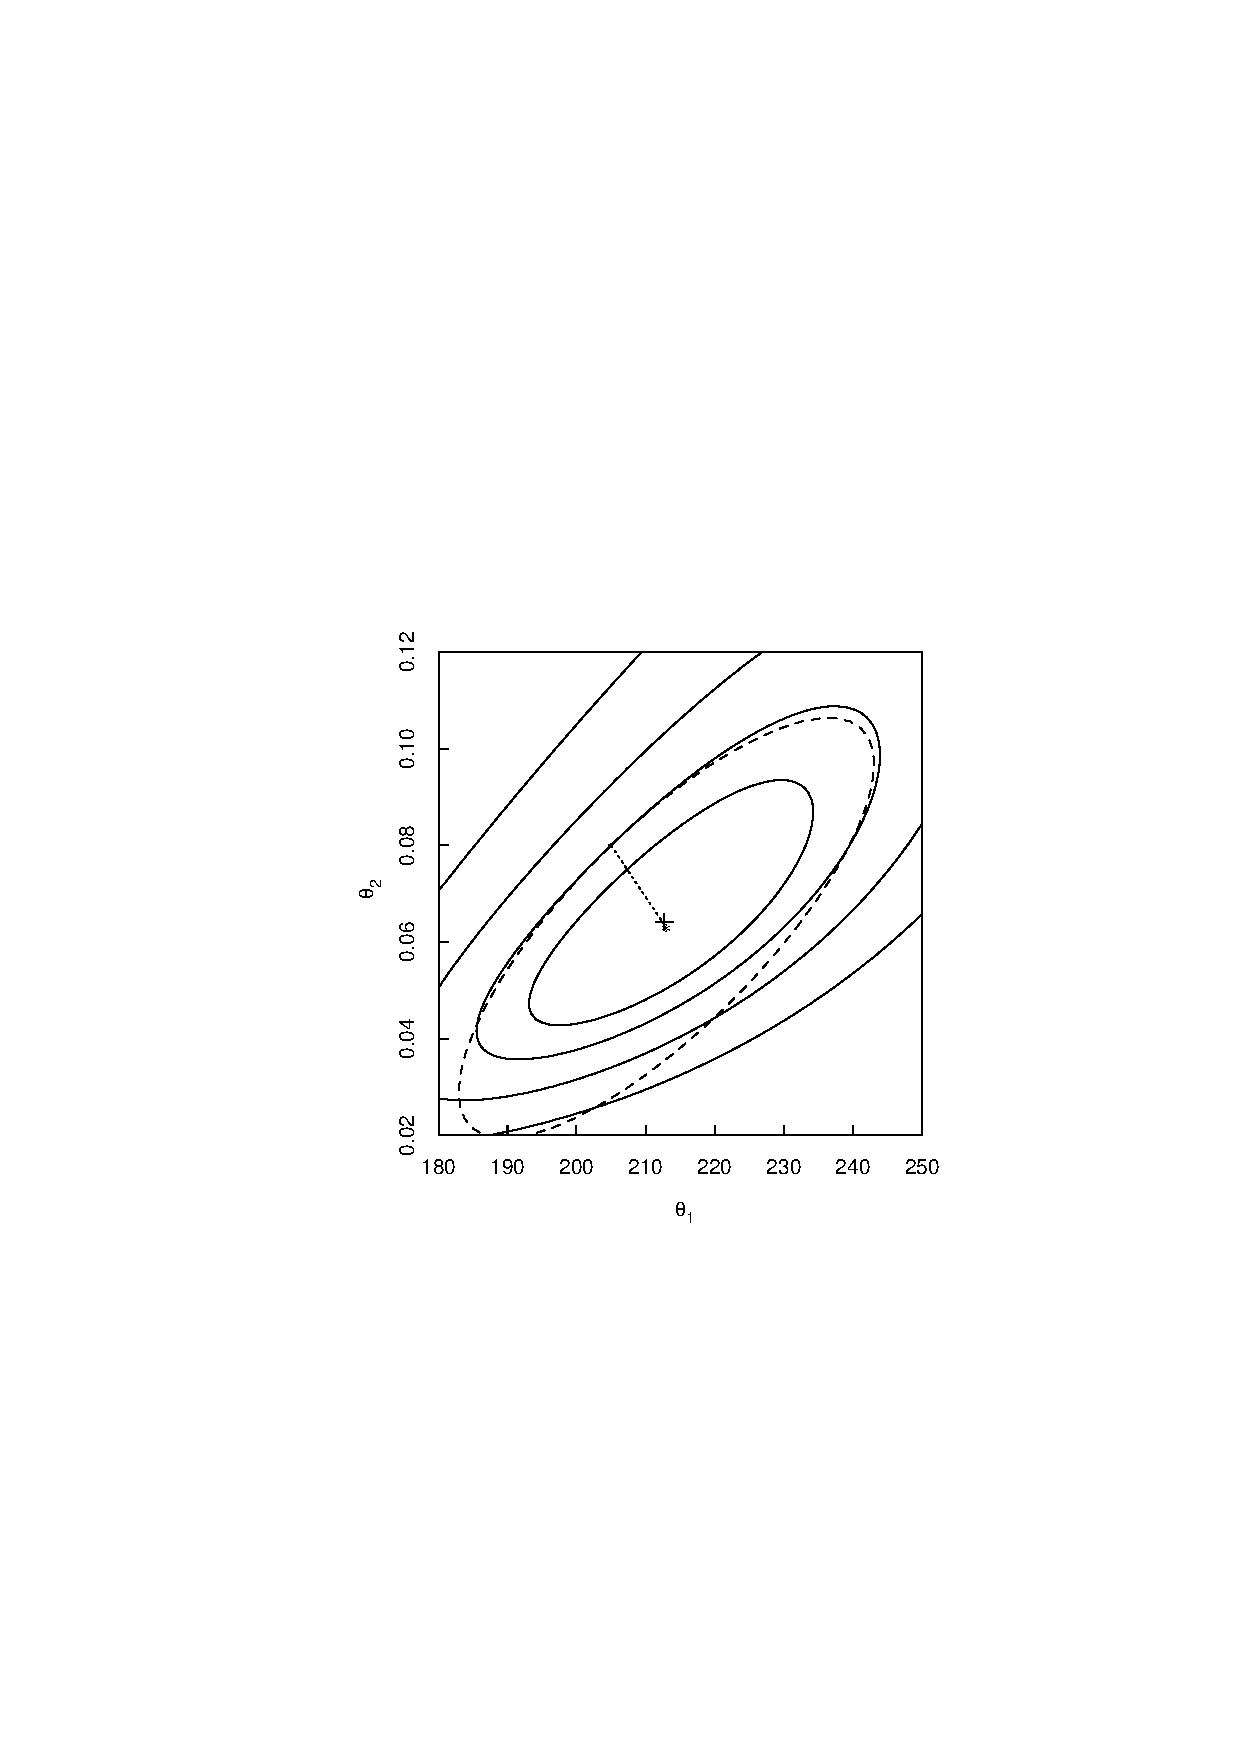
\includegraphics{2MICsumsqinc}}%,width=\textwidth}}
    \caption[Sum of squares contours for Puromycin data]{
    \label{fig:MICsumsqinc}
    Sum of squares contours for the Puromycin data.
    True sum of squares contours are shown as solid lines, and the
    elliptical approximate contour from the linear approximation at
    $\btheta^0=(205,0.08)\trans$ is shown as a dashed line.
    The location of the minimum sum of squares ($+$) and the center of the
    ellipse ($*$) are also shown.
    The dotted line is the Gauss--Newton increment.
    }
  \end{figure}
$S ( \btheta )$, for the Puromycin data, shown as solid lines, and the
location of the minimum, shown as $+$.
Also shown, as a dashed line, is the ellipse derived from the linear
approximation to the expectation function at
$\btheta^0 = ( 205 ,0.08 ) \trans$.
The approximating paraboloid has the
same value and curvature at $\btheta^0$ as the true sum of squares
surface, and so the location of the minimum of the paraboloid,
denoted by $*$,
is used as the apparent minimum of the true sum
of squares surface.
The Gauss increment is therefore the vector joining the starting
point $\btheta^0$ to the point indicated by $*$.

Because the model--data set combination is not badly nonlinear,
the sums of squares contours are quite elliptical, and the
minimum of the approximating paraboloid is near the minimum of
the true sum of squares surface.
\end{example}
\label{bod:BODsumsq}
\begin{example}
  \begin{figure}
    \centerline{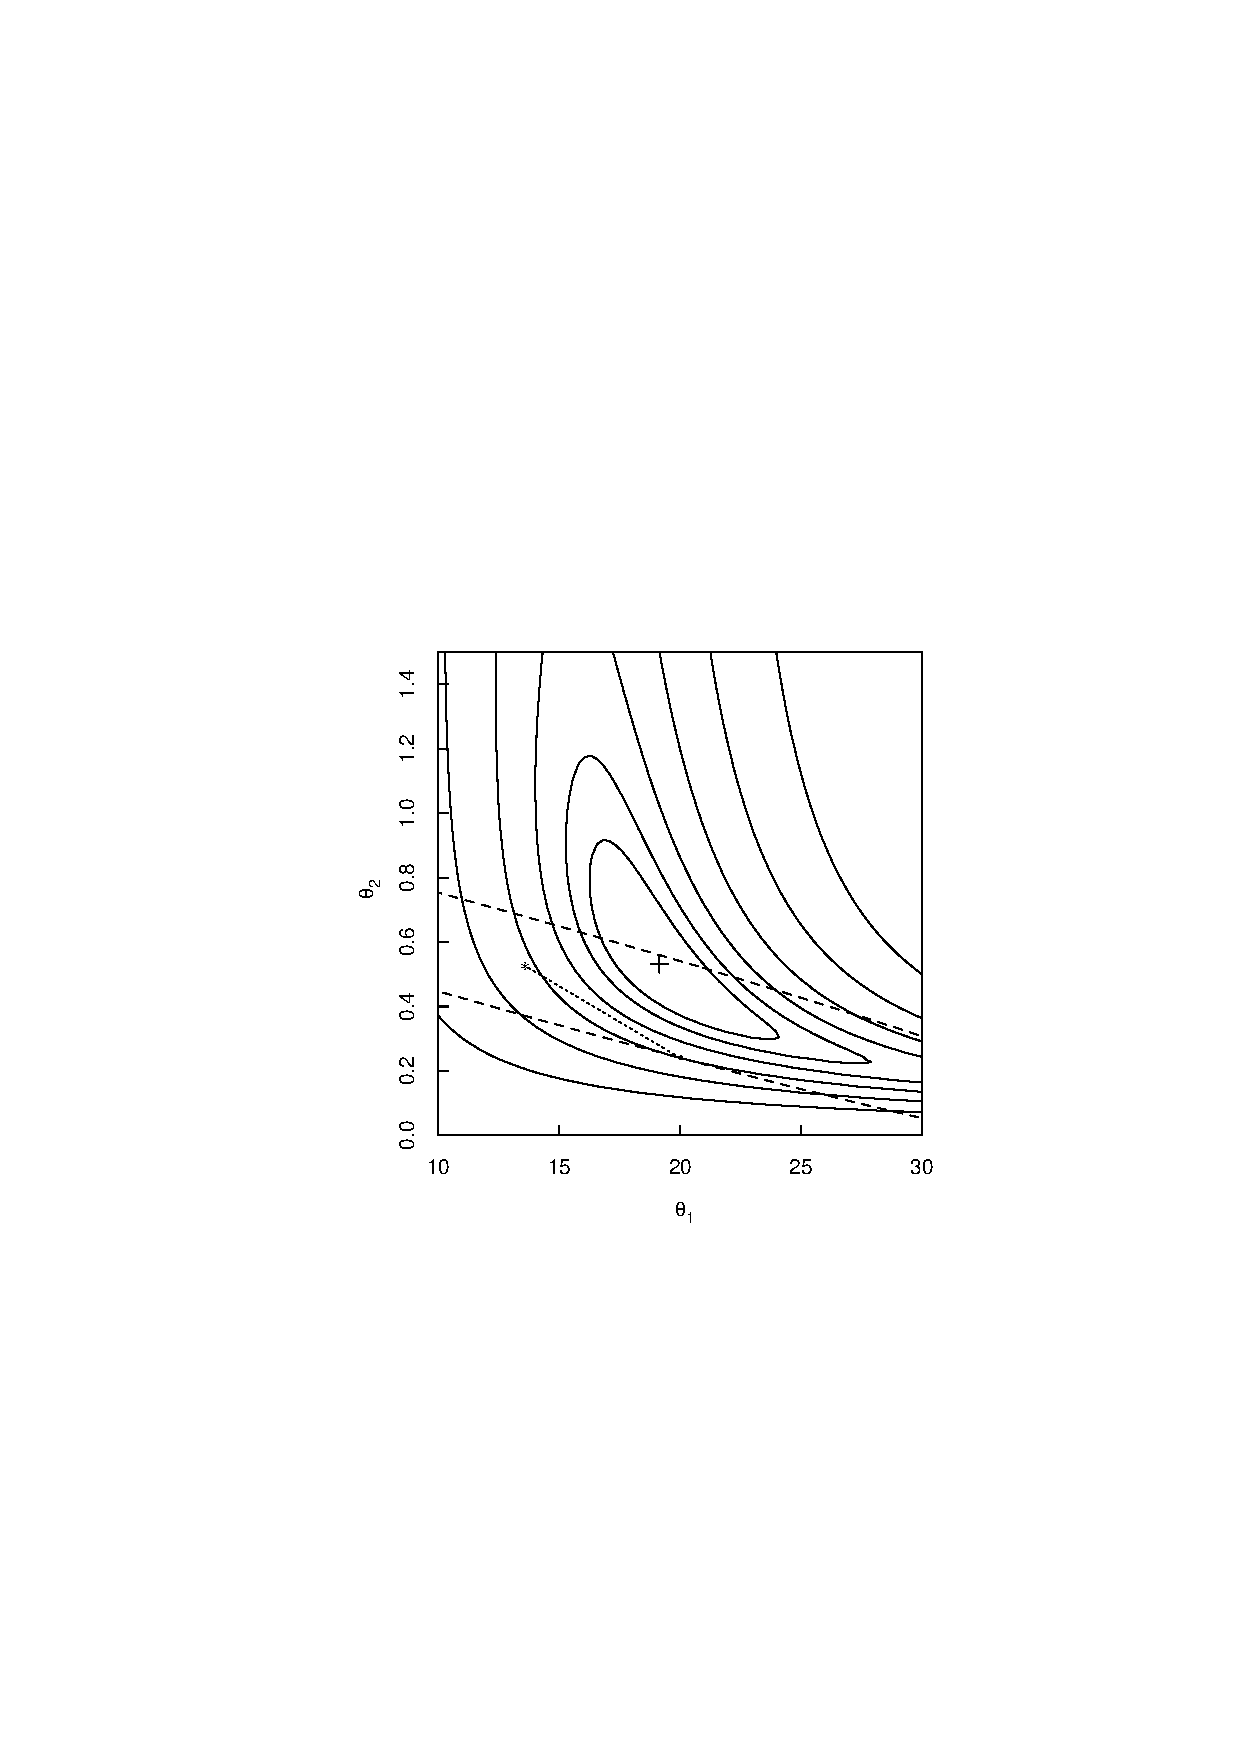
\includegraphics{2BODsumsq}}%,width=\textwidth}}
    \caption[Sum of squares contours for BOD data.]{
    \label{fig:BODsumsq}
    Sum of squares contours for the BOD data.
    True sum of squares contours are shown as solid lines, and a portion of
    the elliptical approximate contour from the linear approximation at
    $\btheta^0=( 20 ,0.24 ) \trans$ is shown as a dashed line.
    The location of the minimum sum of squares ($+$) and the center of the
    ellipse ($*$) are also shown.
    The dotted line is the Gauss--Newton increment.
    }
  \end{figure}
In Figure \ref{fig:BODsumsq} we plot sum of squares contours,
$S ( \btheta )$, for the BOD data, shown as solid lines, and
location of the minimum, shown as $+$.
Also shown, as a dashed line, is a portion of the ellipse derived from
the linear approximation to the expectation function at
$\btheta^0 = ( 20 ,0.24 ) \trans$.
The center of the ellipse is indicated by $*$.

In this example, the ellipse is a poor approximation to the true
contour.
\index{ellipse!approximation to sum of squares contour}
The center of the ellipse is not close to the minimum of the true
sum of squares surface and
furthermore has a true sum of squares greater than that at $\btheta^0$.
\end{example}
\subsection{Overshoot}
\index{overshoot}

The next iteration is carried out from the location of the
apparent minimum of the sum of squares surface---provided, of
course, that $S ( \btheta^1 )$ is less than
$S ( \btheta^0 )$.
In the Rumford example and in the Puromycin example,
because the nonlinearity is moderate,
the sum of squares at $\btheta^1$ is less
than that at $\btheta^0$, and so we can proceed to iterate
from $\btheta^1$.
For the BOD example, however, the sum of squares at
$\btheta^1$ is greater than that at
$\btheta^0$, so we have overshot the
minimum.
By incorporating a step factor, so that only a fraction of the increment
\index{step factor}
is used, we can find
a point with a smaller sum of squares, as described in Section 2.2.1.

\begin{problems}
  \prob
  Write a computer routine in a language of your choice to
  perform nonlinear least squares using the Gauss--Newton approach.
  Take the function, its derivatives with respect to the
  parameters, and starting values as input to the routine.
  If necessary, use the pseudocode in Appendix 3, Section A3.1
  for guidance.

  \prob
  Use a nonlinear least squares routine to fit a model of the form
  $\beta_1+\beta_2(\mbox{\rm age})^{\alpha}$ to the $\ln(\mbox{\rm PCB})$ data.
  Use starting values of $(-2.4,2.3,0.33)\trans$ (the least squares
  estimates for $\beta_1 ,\beta_{2}$ for $\alpha=0.33$ from
  Example PCB 2).

  \prob
  \subprob
  Plot the expectation surface for the Rumford model,
  using the design $\bx = ( 7,  28 ) \trans$.
  Mark the points on the expectation surface
  corresponding to the values
  $\theta=0,0.01,\ldots,0.1,0.2,\ldots,1.0,\infty$.
  Compare this expectation surface with the one based on
  the design $\bx = ( 4,  41 ) \trans$ plotted in Figure 2.3.
  Which design has smaller overall intrinsic nonlinearity?
  Which design has smaller overall parameter effects
  nonlinearity?
  
  \subprob                
  Plot the expectation surface for the Rumford model,
  using the design $\bx = ( 12,  14 ) \trans$.
  Mark the points on the expectation surface
  corresponding to the values
  $\theta=0,0.01,\ldots,0.1,0.2,\ldots,1.0,\infty$.
  Compare this expectation surface with the one based on
  the design $\bx=(4,41)\trans$ plotted in Figure 2.3 and
  with that from part (a).
  Which design has smallest overall intrinsic nonlinearity?
  Which design has smallest overall parameter effects
  nonlinearity?

  \subprob
  What kind of design would have zero intrinsic nonlinearity
  everywhere?  Why?

  \subprob
  Would the design in part (c) have zero parameter
  effects nonlinearity?  Why?

  \prob
  \subprob
  Plot the expectation surface for the linear model
  $\ln(\mbox{\rm PCB})=\beta\ln(\mbox{\rm age})$ for the design
  $\mbox{\rm age}=5,10$.
  Mark the points on the surface corresponding to
  $\beta=0,1,2,3$.

  \subprob
  Compare this expectation surface and its properties
  with those of the nonlinear Rumford model shown in
  Figure 2.3.

  \subprob
  Compare this expectation surface and its properties
  with those of the nonlinear Rumford model plotted in
  Problem 2.3.

  \prob
  \subprob
  Generate the expectation vector, the residual vector,
  the sum of squares  $S ( \btheta^0 )$, and the
  derivative matrix $\bV^{0}$ for the data and model
  from Appendix 4, Section A4.1, at the starting values
  $\btheta^0 = ( 2.20, 0.26 ) \trans$.

  \subprob
  Calculate the increment $\bdelta^0$ and
  $S(\btheta^1)$, where
  $\btheta^1=\btheta^0+\lambda\bdelta^{0}$, for
  $\lambda=0.25,0.50$, and $1.0$.
  Is a step factor less than 1 necessary in this case?

  \prob
  \subprob
  Use the fact that, for the model in Problem 2.5,
  $\theta_{1}$ is conditionally linear, and generate and
  plot exact sum of squares contours for the data in
  Appendix 4, Section A4.1.
  (That is, for any specified value of $\theta_{2}$, it
  is possible to use linear least squares to obtain the
  conditional estimate $\tilde \theta_{1}$ and to
  calculate the values of $\theta_{1}$ which produce a
  specified sum of squares.
  By specifying the sum of squares to be that
  corresponding to a contour value, it is possible to
  generate the exact coordinates of points on the contour.)
  Let $\theta_{2}$ go from 0.12 to 0.3 in steps of 0.01,
  and use contour values corresponding to 50, 75, and
  95\% confidence levels.
  Mark the location of the minimum on the plot.

  \subprob
  Compare these contours with those in Figure 2.23.
  Which data set suffers most from nonlinearity?

  \subprob
  Since the data are from the same type of experiment
  with the same model, how can this difference be
  explained?

  \prob
  Plot the point corresponding to $\btheta^{0}$ and the
  increment $\bdelta^{0}$ from Problem 2.5 on the contour plot
  from Problem 2.6.
  Mark the points corresponding to the values
  $\lambda=0.25,0.5$, and 0.75 on the increment vector.
  Is a step factor less than 1 necessary in this case?

  \prob
  \subprob
  Use the data, model, and starting values from Problem
  2.5 in a nonlinear estimation routine to obtain the
  least squares parameter estimates.

  \subprob
  Calculate and plot the linear approximation joint and
  marginal inference regions on the plot from Problem
  2.6.

  \subprob
  Are the linear approximation inference regions
  accurate in this case?

\end{problems}

% Local Variables: 
% mode: latex
% TeX-master: "nraia2"
% End: 
